\documentclass[10 pt,a4paper, openany]{article}
%titlepage
\usepackage[hidelinks]{hyperref}
\usepackage[italian]{babel}
\usepackage[T1]{fontenc}
\usepackage[utf8x]{inputenc}
\usepackage{amsfonts}
\usepackage{multicol}
\usepackage{graphicx}
\usepackage{amsmath}
\usepackage{framed}
\usepackage{extarrows}
\usepackage{cancel}
\usepackage{eurosym}
\usepackage{listingsutf8}
\usepackage{lastpage}
\usepackage{caption}
\usepackage{csquotes}
\usepackage{makecell}
\usepackage{longtable}
\usepackage{array}
\usepackage{rotating}
\usepackage{placeins}
\usepackage{rotating}
\usepackage{multirow}
\date{}
\newcommand{\normediprogetto}{\emph{Norme di Progetto v4.0.0}}
\newcommand{\studiodifattibilita}{\emph{Studio di Fattibilità v1.0.0}}
\newcommand{\analisideirequisiti}{\emph{Analisi dei Requisiti v4.0.0}}
\newcommand{\definizionediprodotto}{\emph{Definizione di prodotto v3.0.0}}
\newcommand{\gloss}{\emph{Glossario v4.0.0}}
\newcommand{\pianodiprogetto}{\emph{Piano di progetto v4.0.0}}
\newcommand{\pianodiqualifica}{\emph{Piano di qualifica v4.0.0}}



\usepackage{makeidx}
\makeindex
\usepackage{fancyhdr}
\pagestyle{fancy}
\lhead{
\includegraphics[width=.6cm]{../../../file_comuni/immagini/obelisk_sample_02.png}
  Obelix Group}
\chead{}
\rhead{\leftmark }% \leftmark}%da rimettere
\lfoot{}
\cfoot{}
\rfoot{\thepage / \pageref*{LastPage}}
%%%%%%%%%%%%%%%%%%%%%%%%%%%%%%%%%%%%%%
%\usepackage{lipsum}
\usepackage{../../../file_comuni/copertina}
\nomedoc{Definizione di Prodotto}
\versione{v3\_0\_0}
\datacreazione{2017-05-01}
\verifica{Tomas Mali}
\approvazione{Emanuele Crespan}
\redazione{ Nicolò Rigato \eanche Federica Schifano}
\uso{Interno}
\distribuzione{Prof. Tullio Vardanega \eanche Prof. Riccardo Cardin \eanche Gruppo Obelix}
\sommario{Questo documento descrive l’architettura generale e di dettaglio del prodotto Monolith che verrà
  sviluppato dal gruppo Obelix.}



\begin{document}

%

\newcommand{\glossario}[1]{\emph{#1}\ped{|G|}}




%%%%%%%%%%%%%%%%%%%%%%%%%%%%%%%%%%%%%%%%%%%%%%%%%%%%%%%%%%%%%%%%%%%%%%%%%%%%%%%%%%%%%%%%%%%%%%%%%%%%%%%%%%%%%%%%
%%%%% VARIABILI DELLA PAGINA DI TITOLO
\newcommand{\eanche}{\\ &}
\newcommand{\nomedoc}[1]{\gdef\@nomedoc{#1}}
\newcommand{\versione}[1]{\gdef\@versione{#1}}
\newcommand{\datacreazione}[1]{\gdef\@datacreazione{#1}}
\newcommand{\verifica}[1]{\gdef\@verifica{#1}}
\newcommand{\approvazione}[1]{\gdef\@approvazione{#1}}
\newcommand{\redazione}[1]{\gdef\@redazione{#1}}
\newcommand{\uso}[1]{\gdef\@uso{#1}}
\newcommand{\distribuzione}[1]{\gdef\@distribuzione{#1}}
\newcommand{\sommario}[1]{\gdef\@sommario{#1}}
\newcommand{\listaDistribuzione}[1]{\gdef\@listaDistribuzione{#1}}
%%%%%%%%%%%%%%%%%%%%%%%%%%%%%%%%

\newcommand{\paginatitolo}{%
  \begin{titlepage}

    
\includegraphics[width=0.18\textwidth]{../../../file_comuni/immagini/monolith.png}\\[0.08in]

    \begin{center}

      
\includegraphics[width=0.22\textwidth]{../../../file_comuni/immagini/obelisk_sample_02.png}\\[0.08in]
                      {\Large Obelix Group \\% \vspace{.01in}
                        obelixswe@gmail.com \\}
                      \vspace{.15in}
                             {\textbf{\Huge {\@nomedoc}}}

                             \vspace{.15in}
                             \bgroup
                             \def\arraystretch{1.2}
                             \begin{tabular}{r|l}
                               \textbf{Versione}     & \emph{\@versione}  \\%\hline
                               \textbf{Data creazione} & \@datacreazione  \\%\hline
                               \textbf{Redattori} & \@redazione \\%\hline
                               \textbf{Verificatori} & \@verifica \\%\hline
                               \textbf{Approvazione} & \@approvazione
                               \\%\hline
                               \textbf{Stato} & Approvato \\
                               \textbf{Uso} & \@uso \\
                               \textbf{Distribuzione} & \@distribuzione \\
                             \end{tabular}
                             \egroup

                             \vfill

                             \begin{abstract}
                               \@sommario
                             \end{abstract}

    \end{center}
  \end{titlepage}
}
\endinput

\paginatitolo

\section*{Diario delle revisioni}

\begin{center}
	\begin{longtable}{|
			*{1}{>{\centering\arraybackslash}p{1.4 cm}|}
			*{1}{>{\centering\arraybackslash}p{4.5 cm}|}
			*{1}{>{\centering\arraybackslash}p{2.7 cm}|}
			*{1}{>{\centering\arraybackslash}p{1.8 cm}|}}
		
		\hline
		\textbf{Versione} & \textbf{Modifica} & \textbf{Autore e Ruolo} & \textbf{Data} 
		\\
		\hline \endhead
		\hline \endfoot
		\hline 2.0.0 & Approvazione documento & \makecell{Nicolò Rigato\\ Responsabile} & 2017-08-04  \\
		\hline 1.2.1 & Modifica tracciamento & \makecell{Tomas Mali\\ Progettista} & 2017-08-03  \\
		\hline 1.2.0 & Verifica sezioni "Diagrammi di attività" e "Diagrammi di sequenza" & \makecell{Federica Schifano\\ Verificatore} & 2017-08-02 \\
		\hline 1.1.2 & Modifica sezione 6 "Diagrammi di sequenza" & \makecell{Emanuele Crespan\\ Progettista} & 2017-07-31  \\
		\hline 1.1.1 & Modifica sezione 5 "Diagrammi di attività" & \makecell{Riccardo Saggese\\ Progettista} & 2017-07-25  \\
		\hline 1.1.0 & Verifica sezione 3 "Descrizione Architettura" & \makecell{Silvio Meneguzzo\\ Verificatore} & 2017-07-23  \\
		\hline 1.0.10 & Modifica sottosezione 3.5 "Architettura di dettaglio-classi delle bolle Demo" & \makecell{Tomas Mali\\ Progettista} & 2017-07-22  \\
		\hline 1.0.9 & Modifica sottosezione 3.5 "Architettura di dettaglio-classi delle bolle Demo" & \makecell{Riccardo Saggese\\ Progettista} & 2017-07-21  \\
		\hline 1.0.8 & Modifica sottosezione 3.3 "Architettura generale-Bolle Demo" & \makecell{Tomas Mali\\ Progettista} & 2017-07-20  \\
		\hline 1.0.7 & Modifica sottosezione 3.3 "Architettura generale-Bolle Demo" & \makecell{Riccardo Saggese\\ Progettista} & 2017-07-18  \\
		\hline 1.0.6 & Modifica sottosezione 3.4 "Architettura di Dettaglio-Classi del sistema Monolith" & \makecell{Emanuele Crespan\\ Progettista} & 2017-07-18 \\
		\hline 1.0.5 & Modifica sottosezione 3.4 "Architettura di Dettaglio-Classi del sistema Monolith" & \makecell{Tomas Mali\\ Progettista} & 2017-07-18  \\
		\hline 1.0.4 & Modifica sottosezione 3.2 "Architettura generale-Componenti del sistema" & \makecell{Emanuele Crespan\\ Progettista} & 2017-07-17  \\
		\hline 1.0.3 & Modifica sottosezione 3.2 "Architettura generale-Componenti del sistema" & \makecell{Tomas Mali\\ Progettista} & 2017-07-16 \\
		\hline 1.0.2 & Modifica sottosezione 3.2 "Architettura generale-Componenti del sistema" & \makecell{Emanuele Crespan\\ Progettista} & 2017-07-15  \\
		\hline 1.0.1 & Modifica sottosezione 2.7 "Node.js" & \makecell{Riccardo Saggese\\ Progettista} & 2017-07-01  \\
		\hline 1.0.0 & Approvazione documento & \makecell{Riccardo Saggese\\ Responsabile} & 2017-06-19  \\
		\hline 0.16.3 & Aggiunta Appendice & \makecell{Nicolò Rigato\\ Progettista} & 2017-06-18  \\
		\hline 0.16.2 & Aggiunta tracciamento Classi-Requisiti e Requisiti-Classi & \makecell{Federica Schifano\\ Progettista} & 2017-06-18  \\
		\hline 0.16.1 & Aggiunta tracciamento Componenti-Requisiti e Requisiti-Componenti & \makecell{Federica Schifano\\ Progettista} & 2017-06-18  \\
		\hline 0.16.0 & Verifica sezione Diagrammi di sequenza & \makecell{Silvio Meneguzzo\\ Verificatore} & 2017-06-17  \\
		\hline 0.0.10 & Stesura sottosezione Voto sondaggio & \makecell{Emanuele Crespan\\ Progettista} & 2017-06-17  \\
		\hline 0.15.3 & Stesura sottosezione Cancellazione bolla voto sondaggio & \makecell{Riccardo Saggese\\ Progettista} & 2017-06-17  \\
		\hline 0.15.2 & Stesura sottosezione Creazione bolla & \makecell{Nicolò Rigato\\ Progettista} & 2017-06-17  \\
		\hline 0.15.1 & Inizio stesura sezione Diagrammi di sequenza & \makecell{Riccardo Saggese\\ Progettista} & 2017-06-17  \\
		\hline 0.15.0 & Verifica classi componenti MeteoBubble, SurveyBubble,TranslationBubble  & \makecell{Silvio Meneguzzo\\ Verificatore} & 2017-06-16  \\
		\hline 0.14.0 & Verifica classi componenti CurrencyBubble,DiceBubble,ListBubble   & \makecell{Nicolò Rigato\\ Verificatore} & 2017-06-16  \\
		\hline 0.13.6 & Descrizione classi componente TranslationBubble  & \makecell{Federica Schifano\\ Progettista} & 2017-06-16  \\
		\hline 0.13.5 & Descrizione classi componente SurveyBubble  & \makecell{Nicolò Rigato\\ Progettista} & 2017-06-16  \\
		\hline 0.13.4 & Descrizione classi componente MeteoBubble  & \makecell{Emanuele Crespan\\ Progettista} & 2017-06-15  \\
		\hline 0.13.3 & Descrizione classi componente ListBubble  & \makecell{Silvio Meneguzzo\\ Progettista} & 2017-06-15  \\
		\hline 0.13.2 & Descrizione classi componente DiceBubble  & \makecell{Tomas Mali\\ Progettista} & 2017-06-14  \\
		\hline 0.13.1 & Descrizione classi componente CurrencyBubble  & \makecell{Tomas Mali\\ Progettista} & 2017-06-13  \\
		\hline 0.13.0 & Verifica componenti Sideareas,UI-Layouts, UI-SingleComponents  & \makecell{Silvio Meneguzzo\\ Verificatore} & 2017-06-11  \\
		\hline 0.12.3 & Descrizione classi componente UI-SingleComponents  & \makecell{Tomas Mali\\ Progettista} & 2017-06-10  \\
		\hline 0.12.2 & Descrizione classi componente UI-Layouts  & \makecell{Riccardo Saggese\\ Progettista} & 2017-06-06  \\
		\hline 0.12.1 & Descrizione classi componente Sideareas  & \makecell{Federica Schifano\\ Progettista} & 2017-06-06  \\
		\hline 0.12.0 & Verifica componenti Checks e Bubbles  & \makecell{Emanuele Crespan\\ Verificatore} & 2017-06-05  \\
		\hline 0.11.4 & Fine descrizione classi componente Bubbles  & \makecell{Nicolò Rigato\\ Progettista} & 2017-05-29  \\
		\hline 0.11.3 & Fine descrizione classi componente Bubbles  & \makecell{Nicolò Rigato\\ Progettista} & 2017-05-29  \\
		\hline 0.11.2 & Inizio descrizione classi componente Bubbles  & \makecell{Nicolò Rigato\\ Progettista} & 2017-05-27  \\
		\hline 0.11.1 & Descrizione classi componente Checks  & \makecell{Silvio Meneguzzo\\ Progettista} & 2017-05-26  \\
		\hline 0.11.0 & Verifica componenti TranslationBubble e ListBubble  & \makecell{Riccardo Saggese\\ Verificatore} & 2017-05-24  \\
		\hline 0.10.0 & Verifica componenti Currency,Dice,Meteo,Survey Bubble & \makecell{Federica Schifano\\ Verificatore} & 2017-05-23  \\
		\hline 0.9.12 & Descrizione componente ListBubble::CheckListReading & \makecell{Emanuele Crespan\\ Progettista} & 2017-05-23  \\
		\hline 0.9.11 & Descrizione componente ListBubble::CheckListCreation & \makecell{Federica Schifano\\ Progettista} & 2017-05-23  \\
		\hline 0.9.10 & Descrizione componente ListBubble::DataManagement & \makecell{Tomas Mali\\ Progettista} & 2017-05-22  \\
		\hline 0.9.9 & Descrizione componente ListBubble::Configuration & \makecell{Tomas Mali\\ Progettista} & 2017-05-21  \\
		\hline 0.9.8 & Descrizione componente ListBubble::Receiver & \makecell{Nicolò Rigato\\ Progettista} & 2017-05-20  \\
		\hline 0.9.7 & Descrizione componente ListBubble::Sender & \makecell{Nicolò Rigato\\ Progettista} & 2017-05-20  \\
		\hline 0.9.6 & Descrizione componente ListBubble & \makecell{Nicolò Rigato\\ Progettista} & 2017-05-20  \\
		\hline 0.9.5 & Descrizione componente TranslationBubble & \makecell{Federica Schifano\\ Progettista} & 2017-05-19  \\
		\hline 0.9.4 & Descrizione componente SurveyBubble & \makecell{Riccardo Saggese\\ Progettista} & 2017-05-18  \\
		\hline 0.9.3 & Descrizione componente MeteoBubble & \makecell{Silvio Meneguzzo\\ Progettista} & 2017-05-17  \\
		\hline 0.9.2 & Descrizione componente DiceBubble & \makecell{Emanuele Crespan\\ Progettista} & 2017-05-17  \\
		\hline 0.9.1 & Descrizione componente CurrencyBubble & \makecell{Tomas Mali\\ Progettista} & 2017-05-17  \\
		\hline 0.9.0 & Verifica componente UI-SingeComponents & \makecell{Federica Schifano\\ Verificatore} & 2017-05-15  \\
		\hline 0.8.0 & Verifica componente UI-Layouts & \makecell{Federica Schifano\\ Verificatore} & 2017-05-15  \\
		\hline 0.7.0 & Verifica componente SideAreas & \makecell{Riccardo Saggese\\ Verificatore} & 2017-05-15  \\
		\hline 0.6.0 & Verifica componente Bubbles & \makecell{Riccardo Saggese\\ Verificatore} & 2017-05-15  \\
		\hline 0.5.4 & Descrizione componente UI-SingeComponents & \makecell{Silvio Meneguzzo\\ Progettista} & 2017-05-15  \\
		\hline 0.5.3 & Descrizione componente UI-Layouts  & \makecell{Nicolò Rigato\\ Progettista} & 2017-05-14  \\
		\hline 0.5.2 & Descrizione componente SideAreas  & \makecell{Emanuele Crespan\\ Progettista} & 2017-05-14  \\
		\hline 0.5.1 & Descrizione componente Bubbles  & \makecell{Tomas Mali\\ Progettista} & 2017-05-13  \\
		\hline 0.5.0 & Verifica componente Ui & \makecell{Federica Schifano\\ Verificatore} & 2017-05-13  \\
		\hline 0.4.0 & Verifica componenti Monolith e Database & \makecell{Riccardo Saggese\\ Verificatore} & 2017-05-13  \\
		\hline 0.3.7 & Descrizione componente Ui & \makecell{Riccardo Saggese\\ Progettista} & 2017-05-12  \\
		\hline 0.3.6 & Descrizione componente DatabaseSettings & \makecell{Federica Schifano\\ Progettista} & 2017-05-12  \\
		\hline 0.3.5 & Descrizione componente Checks & \makecell{Silvio Meneguzzo\\ Progettista} & 2017-05-12  \\
		\hline 0.3.4 & Descrizione componente Information Storage & \makecell{Emanuele Crespan\\ Progettista} & 2017-05-11  \\
		\hline 0.3.3 & Descrizione componente Database & \makecell{Federica Schifano\\ Progettista} & 2017-05-11  \\
		\hline 0.3.2 & Descrizione componente Monolith & \makecell{Nicolò Rigato\\ Progettista} & 2017-05-10  \\
		\hline 0.3.1 & Stesura sezione Metodo e Formalismo di specifica & \makecell{Tomas Mali\\ Progettista} & 2017-05-09  \\
		\hline 0.3.0 & Verifica sezione Diagrammi Attività  & \makecell{Riccardo Saggese\\ Verificatore} & 2017-05-09  \\
		\hline 0.2.0 & Verifica sezione Standard di Progetto & \makecell{Federica Schifano\\ Verificatore} & 2017-05-08  \\
		\hline 0.1.0 & Verifica prime tre sezioni & \makecell{Riccardo Saggese\\ Verificatore} & 2017-05-08  \\
		\hline 0.0.6 & Stesura sottosezione Configurazione ListBubble & \makecell{Silvio Meneguzzo\\ Progettista} & 2017-05-07  \\
		\hline 0.0.5 & Stesura sottosezione Configurazione sondaggio & \makecell{Federica Schifano\\ Progettista} & 2017-05-06  \\
		\hline 0.0.4 & Inizio stesura sezione Diagrammi Attività & \makecell{Federica Schifano\\ Progettista} & 2017-05-06  \\
		\hline 0.0.3 & Stesura sezione Standard di Progetto & \makecell{Riccardo Saggese\\ Progettista} & 2017-05-05  \\
		\hline 0.0.4 & Inizio stesura sezione Descrizione Architetturale & \makecell{Silvio Meneguzzo\\ Progettista} & 2017-05-04  \\
		\hline 0.0.3 & Stesura sezione Tecnologie Utilizzate & \makecell{Emanuele Crespan\\ Progettista} & 2017-05-03  \\
		\hline 0.0.2 & Stesura sezione Introduzione & \makecell{Federica Schifano\\ Progettista} & 2017-05-02  \\
		\hline 0.0.1 & Creato template & \makecell{Nicolò Rigato\\ Progettista} & 2017-05-01  \\
		\hline
		
	\end{longtable}
\end{center}

%\newpage

%\clearpage


%\hyphenchar\font=-1 % disable hyphen
\tableofcontents
\clearpage
\listoffigures
\listoftables

%\hyphenchar\font=`\- % reset hyphen
\clearpage

%% DEFINIZIONE DI PRODOTTO
%controllare gli svantaggi

\section{Introduzione}
\subsection{Scopo del documento}

Questo documento ha come scopo quello di definire la progettazione ad
alto  e a basso livello
per il prodotto Monolith. Verranno presentate l'architettura generale e
di dettaglio secondo le quali
saranno organizzate le varie componenti software e i \glossario{Design Pattern} utilizzati nella
creazione dell'SDK, delle bolle predefinite e della demo. Verrà
inoltre dettagliato il tracciamento tra le componenti software
individuate ed i requisiti, i requisiti e i componenti, le classi e i
requisiti e i requisiti e le classi.


\subsection{Scopo del prodotto}

Lo scopo del prodotto è quello di permettere la creazione di bolle
interattive, che dovranno funzionare nell'ambiente Rocket.chat. Queste
bolle permetteranno di aumentare l'interattività tra gli utenti della
chat e aggiungeranno nuove funzionalità accessibili direttamente dalla conversazione 
senza il bisogno di ricorrere all'apertura di applicazioni diverse.
Il sistema offrirà agli sviluppatori un set di \glossario{API} per creare e
rilasciare nuove bolle e agli utenti finali la possibilità di
usufruire di un insieme di bolle predefinite.


\subsection{Glossario}

Al fine di evitare ogni ambiguità di linguaggio e massimizzare la
comprensione dei documenti, i termini che necessitano di essere
chiariti saranno scritti in corsivo e marcati con una |G| in pedice alla prima
occorrenza e saranno riportati nel \gloss.

\subsection{Riferimenti}

\subsubsection{Normativi}
\begin{itemize}
	\item \textbf{Norme di Progetto}: \normediprogetto
	\item \textbf{Capitolato d'appalto C5}: \\ \url{http://www.math.unipd.it/~tullio/IS-1/2016/Progetto/C5.pdf}
	\item \textbf{Analisi dei Requisiti}: \analisideirequisiti
	
\end{itemize}


\subsubsection{Informativi}
\begin{itemize}
	\item \textbf{Slide del corso di Ingegneria del Software}:
     	\\  \url{http://www.math.unipd.it/~tullio/IS-1/2016/ }
	\item \textbf{Documentazione React} :  
		\\  \url{https://facebook.github.io/react/docs/installation.html}
	\item \textbf{Documentazione Meteor} : 
		\\  \url{https://guide.meteor.com/}
	\item \textbf{Documentazione ECMAScript 6}  : 
		\\  \url{https://github.com/rse/es6-features} ,
		\\  \url{http://ccoenraets.github.io/es6-tutorial/}
	\item \textbf{Libro Design Patterns} Design Patterns, Elementi per il
  riuso di software a oggetti. Gamma, Helm, Johnson, Vlissides. (Sezioni dedicate ai design pattern utilizzati.)

\end{itemize}

\section{Tecnologie Utilizzate}

In questa sezione verranno descritte le tecnologie su cui si basa lo
sviluppo del progetto. Per ognuna di esse, verranno indicati l’ambito
di utilizzo della tecnologia, i vantaggi e gli svantaggi che ne
derivano. Alcune delle tecnologie che saranno usate sono richieste come requisito dal capitolato scelto.

\subsection{Javascript 6th edition (ECMA SCRIPT 6)}

JavaScript è un \glossario{linguaggio di scripting} orientato agli oggetti e agli
eventi. \'E comunemente utilizzato nella programmazione Web lato
client per la creazione, in siti web e applicazioni web, di effetti
dinamici interattivi tramite l'uso di funzioni di script invocate da
eventi innescati in vari modi dall'utente sulla pagina web in
uso. \\ Come richiesto dal capitolato, per la realizzazione di
Monolith, deve essere utilizzato \glossario{Javascript} 6th edition (ECMA SCRIPT
6). \\ 

\paragraph{Licenza}  
Non esiste una sola implementazione perché ECMAScript (o ES) è un
linguaggio di programmazione standardizzato e mantenuto da Ecma
International nell'ECMA-262 ed ISO/IEC 16262. \\


\paragraph{Vantaggi}
\begin{itemize}
	\item Gestione degli eventi asincroni tramite le promises
	\item Possibilità di dichiarare classi
	\item Supporto per le costanti(\emph{const})
	\item Possibilità di isolare la definizione di variabili ad un blocco (\emph{let})
	\item Possibilità di isolare lo scope di una funzione usando
     blocchi delimitati da parentesi graffe \{\} come ambienti isolati (vs closure)
	\item Uso di sintassi più espressiva per scrivere le funzioni anonime (\emph{Arrow Functions})
	
\end{itemize}

\paragraph{Svantaggi} 
\begin{itemize}
	\item Il supporto di ES6 da parte dei browser è ancora incompleto
	\item L’assenza di tipizzazione potrebbe ostacolare la valutazione della correttezza del codice
\end{itemize}

\subsection{Meteor}

Meteor è un framework web JavaScript libero e open source  per lo
sviluppo di applicazioni web e mobile. \'E una piattaforma basata su
Node.js. Meteor utilizza, dunque, JavaScript sia lato client che lato
server.  
\\
\paragraph{Licenza} MIT 
La licenza MIT è una delle licenze più permissive nel panorama open
source. In modo più esplicito dichiara i diritti dati all'utente
finale, incluso il diritto di utilizzare, copiare, modificare,
incorporare, pubblicare, distribuire, sotto-licenziare, e/o vendere il
software. 


\paragraph{Vantaggi}
\begin{itemize}
	\item Integrazione con diverse tecnologie utilizzate nello sviluppo web:
	\begin{itemize}
		\item React
		\item MongoDB
	\end{itemize}
	\item Isomorfismo: il codice javascript scritto funziona in modo trasparente sul client (browser), sul server (Node.js) o in entrambi
	\item Ecosistema e modularità: la comunità di Meteor è molto attiva
     e molte funzionalità client o server potrebbero già essere
     pacchettizzate dal \glossario{package} manager ufficiale 
\end{itemize}

\paragraph{Svantaggi} %controllareeeeeee 
\begin{itemize}
	\item Inizialmente sconosciuto ai membri del gruppo.
	%\item Il modo in cui alcuni componenti core della tecnologia si interfacciano potrebbe limitare la libertà degli sviluppatori.
\end{itemize}

\subsection{Mongo DB}
MongoDB è un database NoSQL orientato ai documenti, basato sul formato \glossario{BSON} per la memorizzazione e la rappresentazione dei dati. \'E distribuito come software libero open source. \\

\paragraph{Licenza} GNU AGPL v3.0 \\
\'E una licenza pubblicata da Free Software Foundation. \'E simile alla capostipite GNU GPL, una licenza fortemente copyleft per software libero.

\paragraph{Vantaggi}
\begin{itemize}
	\item \'E più flessibile di un database \glossario{SQL} e facilita la rappresentazione su un modello ad
	oggetti
	\item Supporta ricerche per campi, intervalli e regular expression. Le query possono restituire campi specifici del documento e anche includere funzioni definite dall'utente in JavaScript.
	\item Qualunque campo in MongoDB può essere indicizzato 
\end{itemize}


\paragraph{Svantaggi} 
\begin{itemize}
	\item Inizialmente sconosciuto ai membri del gruppo
     \item Non è possibile eseguire query complesse a causa
       dell'assenza di schema dei dati. A causa di questo parte della
       complessità non può essere demandata al sistema di database
\end{itemize}

\subsection{HTML5}
HTML5 è un linguaggio di markup per la strutturazione delle pagine web.

\paragraph{Licenza}  
Non esiste una sola implementazione perché HTML5 è un linguaggio di markup standardizzato e mantenuto da W3C.



\paragraph{Vantaggi}
\begin{itemize}
	\item Codice più pulito e sintassi semplificata rispetto alle versioni precedenti
	\item Interattività senza l’ausilio di plugin esterni valida per diversi formati multimediali
	\item Semantica intuitiva grazie ai nuovi \glossario{TAG} di formattazione
	\item Introduzione della geo localizzazione, dovuta ad una forte espansione di sistemi operativi mobili
	\item Sistema più efficiente alternativo ai normali cookie chiamato Web Storage 

\end{itemize}

\paragraph{Svantaggi} 
\begin{itemize}
	\item Non tutti i browser supportano HTML5
\end{itemize}

\subsection{SCSS}

SCSS è una sintassi per i fogli di stile introdotta da Sass 3 (Syntactically Awesome StyleSheets). \'E un'estensione del CSS .

\paragraph{Licenza} MIT \\
La licenza MIT è una delle licenze più permissive nel panorama open
source. In modo più esplicito dichiara i diritti dati all'utente
finale, incluso il diritto di utilizzare, copiare, modificare,
incorporare, pubblicare, distribuire, sotto-licenziare, e/o vendere il
software. 

\paragraph{Vantaggi}
\begin{itemize}
	\item Possibilità di utilizzare variabili
	\item Possibilità di creare funzioni 
	\item Possibilità di organizzare il foglio di stile in più file
	\item Compatibilità completa con la sintassi del CSS
\end{itemize}

\paragraph{Svantaggi} 
\begin{itemize}
	\item  Sintassi più complessa.
\end{itemize}

\subsection{React}

React è una libreria Javascript open source che permette di costruire interfacce utente. 
\\
\paragraph{Licenza} BSD-3-Clause \\
Le licenze BSD sono una famiglia di licenze permissive, senza copyleft, per software.
Le tre clausole della licenza BSD-3-Clause sono:
\\
\begin{itemize}
	\item Libertà di eseguire il programma per qualsiasi scopo
	\item Libertà di studiare il programma e modificarlo
	\item Libertà di ridistribuire copie del programma in modo da aiutare il prossimo
	
\end{itemize}

\paragraph{Vantaggi}
\begin{itemize}
	\item Semplificazione della realizzazione di interfacce UI dinamiche che possono reagire ai cambiamenti di dati in maniera autonoma attraverso opportuni componenti
	\item Possibilità di utilizzare le viste per creare codice più facile da comprendere e su cui è più semplice effettuare il debugging.
	
\end{itemize}

\paragraph{Svantaggi} 
\begin{itemize}
	\item Implementa solo la parte puramente visuale
     dell'applicazione. Esistono alternative che possono gestire molti
     più aspetti.
	\item Curva di apprendimento ripida
	\item \'E una libreria relativamente nuova
\end{itemize}

\subsection{Node.js}

Node.js è una piattaforma event-driven per il motore JavaScript
V8. Essa permette di realizzare applicazioni web utilizzando il
linguaggio JavaScript, che tipicamente è usato client-side, per la scrittura anche
della parte server-side delle applicazioni web. 
\\
\paragraph{Licenza} MIT \\
La licenza MIT è una delle licenze più permissive nel panorama open
source. In modo più esplicito dichiara i diritti dati all'utente
finale, incluso il diritto di utilizzare, copiare, modificare,
incorporare, pubblicare, distribuire, sotto-licenziare, e/o vendere il
software. \\

\paragraph{Vantaggi}
\begin{itemize}
	\item Facile apprendimento
	\item Possibilità di realizzare la parte back-end di applicazioni utilizzando lo stesso linguaggio della parte front-end.
\end{itemize}

\paragraph{Svantaggi} 
\begin{itemize}
	\item Non supporta database relazionali
	
\end{itemize}

\subsection{Rochet.chat}

Rocket.chat è una Web chat server sviluppata in Javascript utilizzando il \glossario{Framework} Meteor.

\paragraph{Licenza} MIT \\
La licenza MIT è una delle licenze più permissive nel panorama open
source. In modo più esplicito dichiara i diritti dati all'utente
finale, incluso il diritto di utilizzare, copiare, modificare,
incorporare, pubblicare, distribuire, sotto-licenziare, e/o vendere il
software. \\

\paragraph{Vantaggi}
\begin{itemize}

	\item Codice open source
	\item Possibilità di creare chat di gruppo
	\item Possibilità di inviare audio, video e file
	\item Possibilità di effettuare video chiamate
	\item Community molto attiva

	
\end{itemize}

\paragraph{Svantaggi} 
\begin{itemize}
	\item Parzialmente documentata
\end{itemize}

\subsection{Bootstrap}

Bootstrap è una raccolta di strumenti liberi per la creazione di siti
e applicazioni per il Web. Essa contiene modelli di progettazione
basati su HTML e CSS, sia per la tipografia, che per le varie
componenti dell'interfaccia, come moduli, pulsanti e navigazione, così
come alcune estensioni opzionali di JavaScript. \\

\paragraph{Licenza} MIT \\
La licenza MIT è una delle licenze più permissive nel panorama open
source. In modo più esplicito dichiara i diritti dati all'utente
finale, incluso il diritto di utilizzare, copiare, modificare,
incorporare, pubblicare, distribuire, sotto-licenziare, e/o vendere il
software. 

\paragraph{Vantaggi}
\begin{itemize}
	
	\item Piattaforma ben standardizzata 
	\item Non richiede l’appoggio né di un linguaggio di programmazione server side, né di un database
	\item Ottima documentazione
	\item \glossario{Responsive} Design	
	\item \'E supportato dai browser moderni
	
\end{itemize}

\paragraph{Svantaggi} 
\begin{itemize}
	\item I plugin di jQuery sono limitati
	\item Le modifiche dovute al continuo sviluppo non sono sempre facili da integrare
\end{itemize}



\subsection{polyglot.js}
Polyglot.js è una libreria per la traduzione scritta in JavaScript, eseguita sia per il browser che per gli ambienti CommonJS(Node).

\paragraph{Licenza} MIT \\
La licenza MIT è una delle licenze più permissive nel panorama open
source. In modo più esplicito dichiara i diritti dati all'utente
finale, incluso il diritto di utilizzare, copiare, modificare,
incorporare, pubblicare, distribuire, sotto-licenziare, e/o vendere il
software. \\

\paragraph{Vantaggi}
\begin{itemize}
	\item Non è richiesta una iscrizione per l'utilizzo
	\item \'E un servizio non a pagamento
	\item Il Polyglot ha zero dipendenze
	\item Copre una traduzione di 30 lingue diverse
\end{itemize}




\subsection{Money.js}

Money.js è una libreria semplice con l'unico obiettivo di convertire
un valore di denaro da qualsiasi valuta in qualsiasi altra
valuta. Money.js utilizza una fusione algoritmica per calcolare un
insieme di tassi costantemente preciso per 165 valute mondiali. 
 \\

\paragraph{Licenza} MIT \\
La licenza MIT è una delle licenze più permissive nel panorama open
source. In modo più esplicito dichiara i diritti dati all'utente
finale, incluso il diritto di utilizzare, copiare, modificare,
incorporare, pubblicare, distribuire, sotto-licenziare, e/o vendere il
software.\\ 

\paragraph{Vantaggi}
\begin{itemize}
	\item Non è richiesta una iscrizione per l'utilizzo
	\item \'E un servizio non a pagamento
	\item \'E una libreria semplice da integrare nel codice JavaScript
\end{itemize}


\subsection{weather.js}

Weather.js è una libreria che recupera i dati da openweathermap.org e
fa la ricerca di tutti i tipi di informazioni relative alle condizioni
meteo. 

\paragraph{Licenza} MIT \\
La licenza MIT è una delle licenze più permissive nel panorama open
source. In modo più esplicito dichiara i diritti dati all'utente
finale, incluso il diritto di utilizzare, copiare, modificare,
incorporare, pubblicare, distribuire, sotto-licenziare, e/o vendere il
software. \\

\paragraph{Vantaggi}
\begin{itemize}
	\item Non è richiesta una iscrizione per l'utilizzo
	\item \'E un servizio non a pagamento
	\item \'E una libreria semplice da integrare nel codice JavaScript
\end{itemize}

\paragraph{Svantaggi} 
\begin{itemize}
	\item Ha bisogno di 11 dipendenze 
\end{itemize}


\subsection{classNames}

classNames è una semplice utility raccomandata per l'uso con \glossario{React} per l'unione condizionata di className

\paragraph{Licenza} MIT \\
La licenza MIT è una delle licenze più permissive nel panorama open
source. In modo più esplicito dichiara i diritti dati all'utente
finale, incluso il diritto di utilizzare, copiare, modificare,
incorporare, pubblicare, distribuire, sotto-licenziare, e/o vendere il
software. 
\\

\paragraph{Vantaggi}
\begin{itemize}
	\item Semplifica la gestione dei className dinamici 
	\item Non possiede ulteriori dipendenze 
\end{itemize}


\subsection{Bluebird}
Bluebird è una libreria di promessa incentrata sulle caratteristiche e le prestazioni innovative.

\paragraph{Licenza} MIT \\
La licenza MIT è una delle licenze più permissive nel panorama open
source. In modo più esplicito dichiara i diritti dati all'utente
finale, incluso il diritto di utilizzare, copiare, modificare,
incorporare, pubblicare, distribuire, sotto-licenziare, e/o vendere il
software. 
\\

\paragraph{Vantaggi}
\begin{itemize}
\item Bluebird fornisce tutti gli strumenti e le utility necessarie per realizzare un DSL altamente espressivo e fluente per il JavaScript asincrono
\item Bluebird esegue praticamente su ogni piattaforma. Ciò rende il bluebird ideale per progetti che si preoccupano di fornire un'esperienza coerente tra piattaforme e cross-version
\end{itemize}


\subsection{Simple-Schema}
Simple-Schema è un semplice pacchetto intelligente per la validazione dello schema reattivo per Meteor.

\paragraph{Licenza} MIT \\
La licenza MIT è una delle licenze più permissive nel panorama open
source. In modo più esplicito dichiara i diritti dati all'utente
finale, incluso il diritto di utilizzare, copiare, modificare,
incorporare, pubblicare, distribuire, sotto-licenziare, e/o vendere il
software. 
\\



\paragraph{Vantaggi}
\begin{itemize}
\item Permettere la definizione della struttura della collezione in modo semplice
\item Non possiede ulteriori dipendenze 
\end{itemize}


\subsection{react-meteor-data}
react-meteor-data è un pacchetto per meteor che fornisce la reattività
dei dati di Meteor ai componenti React

\paragraph{Vantaggi}
\begin{itemize}
\item semplice intergrazione di React in Blaze, di React in Meteor
\item semplice integrazione di nuove collezioni nel funzionamento di
  interfacce grafiche già esistenti
\end{itemize}


\section{Descrizione Architettura}
\subsection{Metodo e formalismo di specifica}

Nell’esposizione dell’architettura dell’applicazione si procederà con
un approccio top-down, descrivendo l’architettura iniziando dal
generale ed andando al particolare. 
Si procederà quindi alla descrizione dei componenti software, per poi descrivere
nel dettaglio le singole classi, specificando per ognuna il tipo, l’obiettivo, la funzione e
le relazioni in ingresso ed in uscita.
Successivamente si illustreranno degli esempi di uso dei Design
Pattern nell’architettura del sistema. 
L'architettura dell' \glossario{SDK} e della \glossario{demo} sono state progettate separatamente.  
Per i diagrammi delle componenti di classe e di attività, si utilizza
il formalismo \glossario{UML} 2.0. Le classi e componenti presenti in librerie o
framework esterni vengono contraddistinte da colori diversi. I
framework esterni verranno rappresentati con un colore azzurro, invece
le classi e componenti proprie saranno rappresentate con un
colore giallo. Nella demo le componenti dell'SDK sono in verde.
L'intera applicazione è progettata utilizzando il framework
\glossario{Meteor} che permette di utilizzare il linguaggio JavaScript
sia per il lato client che per quello server(tramite NodeJS). 
I diagrammi delle classi che permettono di mostrare l’architettura
generale del sistema vengono affiancati anche dai diagrammi di
sequenza e attività, che permettono di definire le interazioni tra le
componenti, senza preoccuparsi della loro classificazione. 

%%  \subsection{Architettura generale - Componenti del sistema}
\subsection{Architettura generale - Componenti del sistema}
\subsubsection{Monolith}
   \FloatBarrier
   \begin{figure}[ht]
   \centering
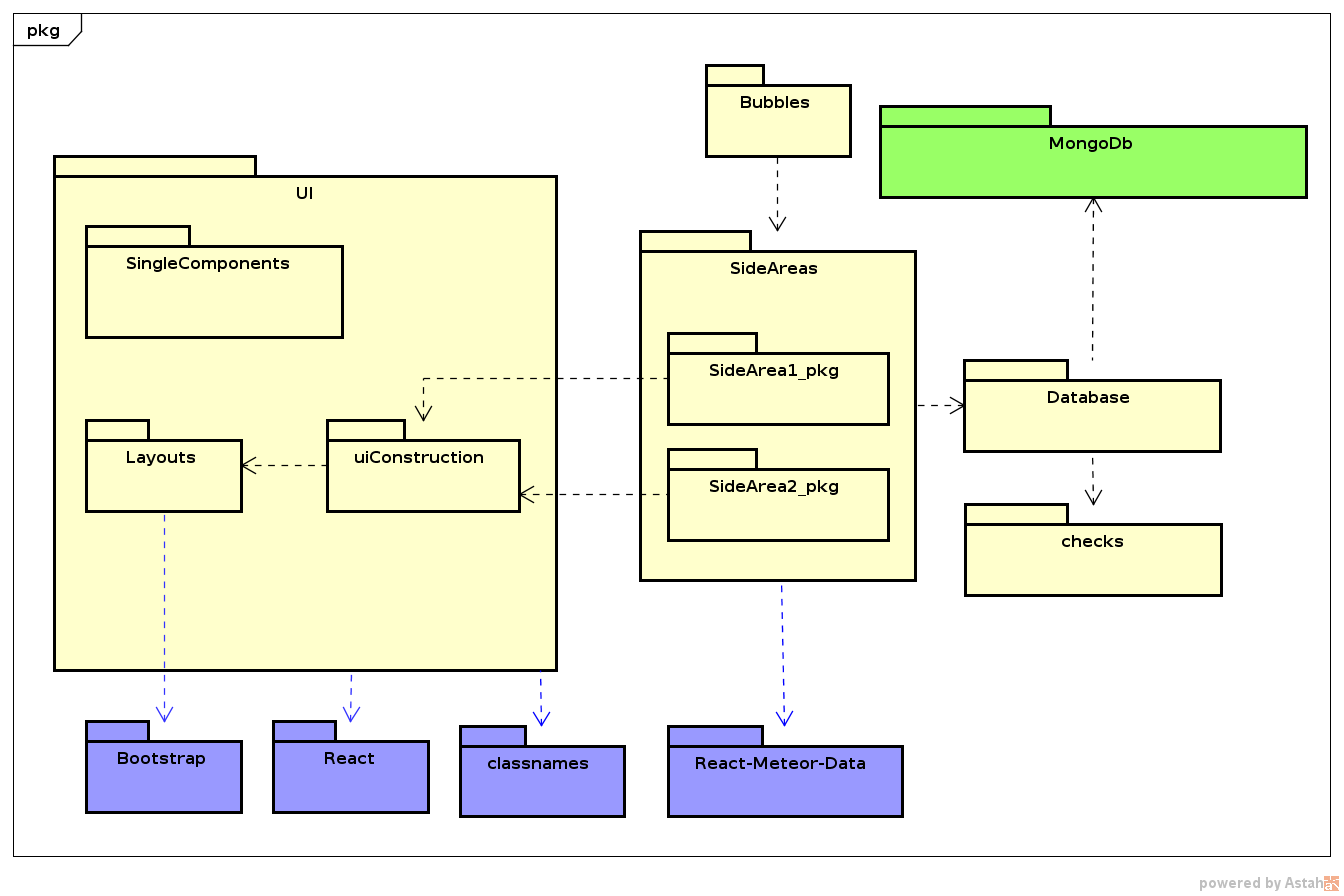
\includegraphics[width=\textwidth,keepaspectratio]{img/General}
   \caption{Diagramma per Monolith.}
\end{figure}
\FloatBarrier
\textbf{Descrizione}:\\
 Componente che rappresenta l'intera SDK di Monolith 


\clearpage

\subsubsection{Monolith::Bubbles}
   \FloatBarrier
   \begin{figure}[ht]
   \centering
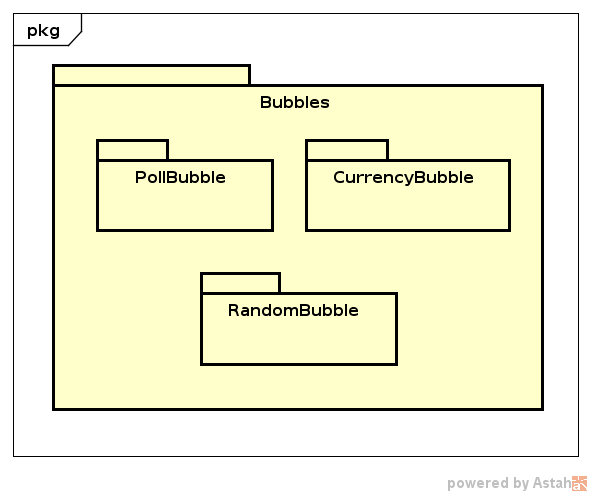
\includegraphics[width=\textwidth,keepaspectratio]{img/Bubbles}
   \caption{Diagramma per Monolith::Bubbles.}
\end{figure}
\FloatBarrier
\textbf{Descrizione}:\\
 Componente che contiene i pacchetti delle bolle predefinite include in Monolith 


\clearpage

\subsubsection{Monolith::checks}
   \FloatBarrier
   \begin{figure}[ht]
   \centering
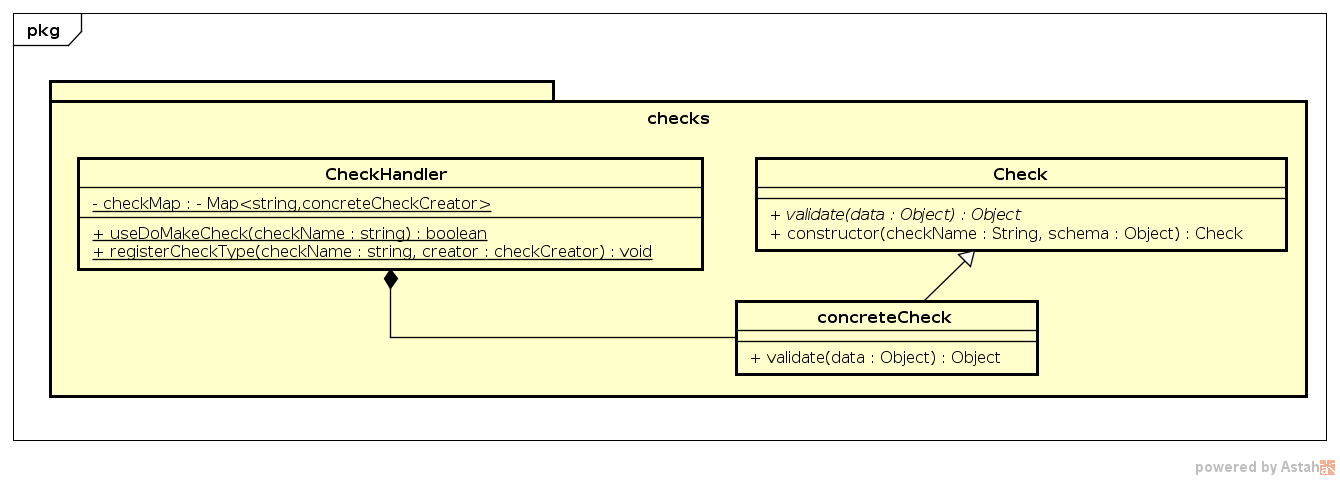
\includegraphics[width=\textwidth,keepaspectratio]{img/controls}
   \caption{Diagramma per Monolith::checks.}
\end{figure}
\FloatBarrier
\textbf{Descrizione}:\\
 Componente che contiene il codice necessario a eseguire controlli sugli input degli utenti. Dipende dalla libreria SimpleSchema. 
\\ \textbf{Classi contenute}:\\
\begin{itemize}
\item Check
\item CheckHandler
\end{itemize}


\clearpage

\subsubsection{Monolith::Database}
   \FloatBarrier
   \begin{figure}[ht]
   \centering
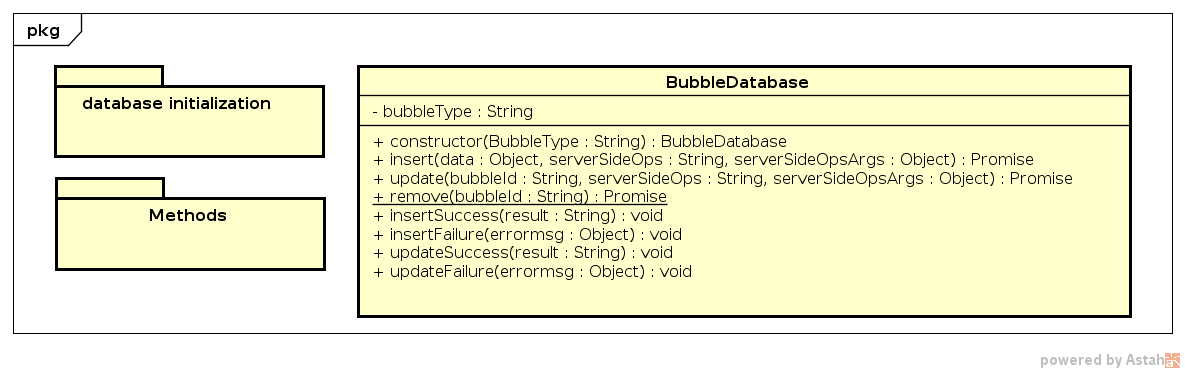
\includegraphics[width=\textwidth,keepaspectratio]{img/database}
   \caption{Diagramma per Monolith::Database.}
\end{figure}
\FloatBarrier
\textbf{Descrizione}:\\
 Componente contenente i pacchetti che vengono utilizzati per interagire con il database 
\\ \textbf{Classi contenute}:\\
\begin{itemize}
\item BubbleDatabase
\end{itemize}


\clearpage

\subsubsection{Monolith::Database::databaseInitialization}
\textbf{Descrizione}:\\
 Componente che si occupa di inizializzare e esportare la collezione che memorizza le bolle e di effettuare la pubblicazione (Meteor.Publish). Viene fornita anche una versione della collezione da utilizzare con il meccanismo delle promises grazie alla libreria Bluebird. 


\clearpage

\subsubsection{Monolith::Database::Methods}
\textbf{Descrizione}:\\
 Componente che contiene i principali Meteor.Methods  che riguardano le bolle:
\\begin{itemize}
\\item insertBubble(bubbleType, roomId, data, funDataEdit, funDataEditArgs) \\\\
Effettua i controlli sull'input tramite il pacchetto Monolith::checks. Aggiunge i dati che devono essere presenti in ogni bolla (indipendentemente dal tipo) e in caso di successo l'operazione viene eseguita sul database.\\\\
Gli ultimi due argomenti sono opzionali e sono il nome di un Meteor.Method e i suoi eventuali argomenti. In caso tale argomento sia presente il metodo indicato viene usato sull'oggetto data prima di effettuare i controlli. In questo modo è possibile stabilire operazioni da svolgere lato server.
\\item updateBubble(bubbleId, funDataEdit, funDataEditArgs)\\\\
\\item removeBubble(bubbleId) \\\\
La bolla con l'id passato come argomento viene eliminata dal database,
\\end{itemize} 


\clearpage

\subsubsection{Monolith::SideAreas}
\textbf{Descrizione}:\\
 Contiene i package per la visualizzazione delle bolle nelle side-bar 


\clearpage

\subsubsection{Monolith::SideAreas::SideArea1\_pkg}
   \FloatBarrier
   \begin{figure}[ht]
   \centering
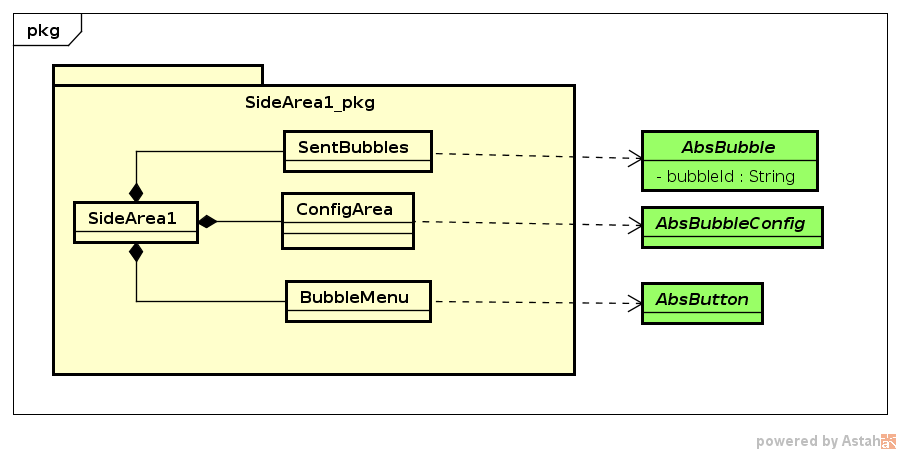
\includegraphics[width=\textwidth,keepaspectratio]{img/sd1_pkg}
   \caption{Diagramma per Monolith::SideAreas::SideArea1\_pkg.}
\end{figure}
\FloatBarrier
\textbf{Descrizione}:\\
 Componente per la visualizzazione delle bolle inviate e del menù di creazione delle bolle nella prima side area 
\\ \textbf{Classi contenute}:\\
\begin{itemize}
\item BubbleMenu
\item ConfigArea
\item SentBubbles
\item SideArea1
\end{itemize}


\clearpage

\subsubsection{Monolith::SideAreas::SideArea2\_pkg}
   \FloatBarrier
   \begin{figure}[ht]
   \centering
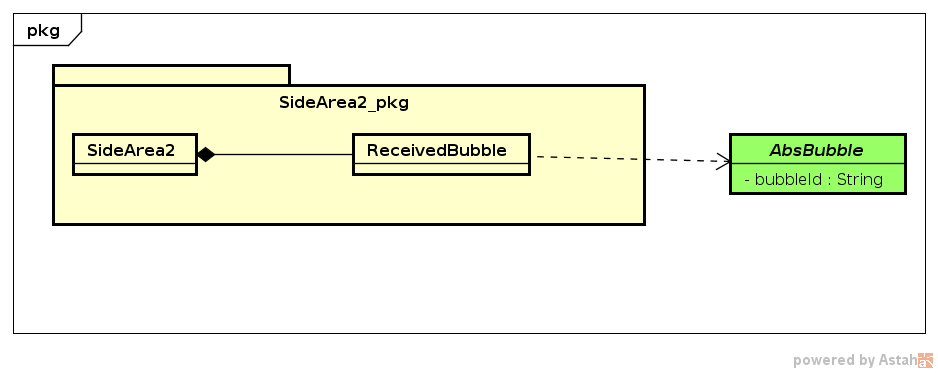
\includegraphics[width=\textwidth,keepaspectratio]{img/sd2_pkg}
   \caption{Diagramma per Monolith::SideAreas::SideArea2\_pkg.}
\end{figure}
\FloatBarrier
\textbf{Descrizione}:\\
 Componente per la visualizzazione delle bolle ricevute nella seconda side area 
\\ \textbf{Classi contenute}:\\
\begin{itemize}
\item ReceivedBubble
\item SideArea2
\end{itemize}


\clearpage

\subsubsection{Monolith::UI}
\textbf{Descrizione}:\\
 Componente contenente tutti i pacchetti che servono per comporre e gestire la parte visuale dell'applicazione delle bolle \\\\
\\textbf{Dipendenze}
\\begin{itemize}
\\item React
\\item classNames
\\end{itemize} 


\clearpage

\subsubsection{Monolith::UI::Layouts}
   \FloatBarrier
   \begin{figure}[ht]
   \centering
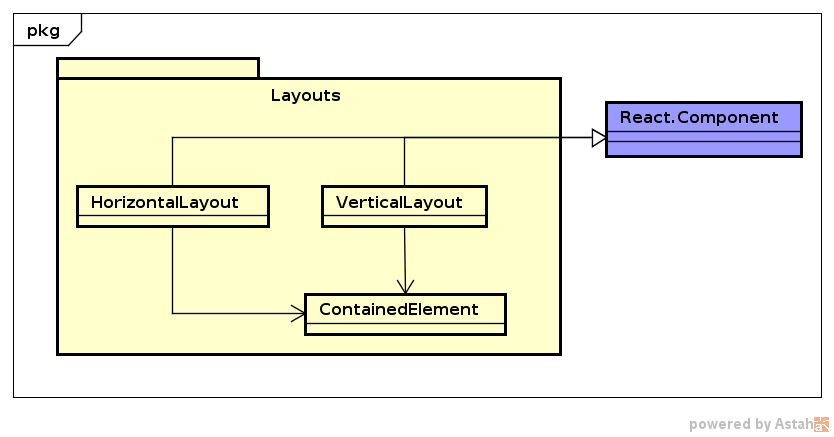
\includegraphics[width=\textwidth,keepaspectratio]{img/UI-Layouts}
   \caption{Diagramma per Monolith::UI::Layouts.}
\end{figure}
\FloatBarrier
\textbf{Descrizione}:\\
 Componente che contiene le classi React per la gestione dei layout \\\\
\textbf{Dipendenze} \\
Bootstrap 
\\ \textbf{Classi contenute}:\\
\begin{itemize}
\item ContainedElement
\item HorizontalLayout
\item VerticalLayout
\end{itemize}


\clearpage

\subsubsection{Monolith::UI::SingleComponents}
   \FloatBarrier
   \begin{figure}[ht]
   \centering
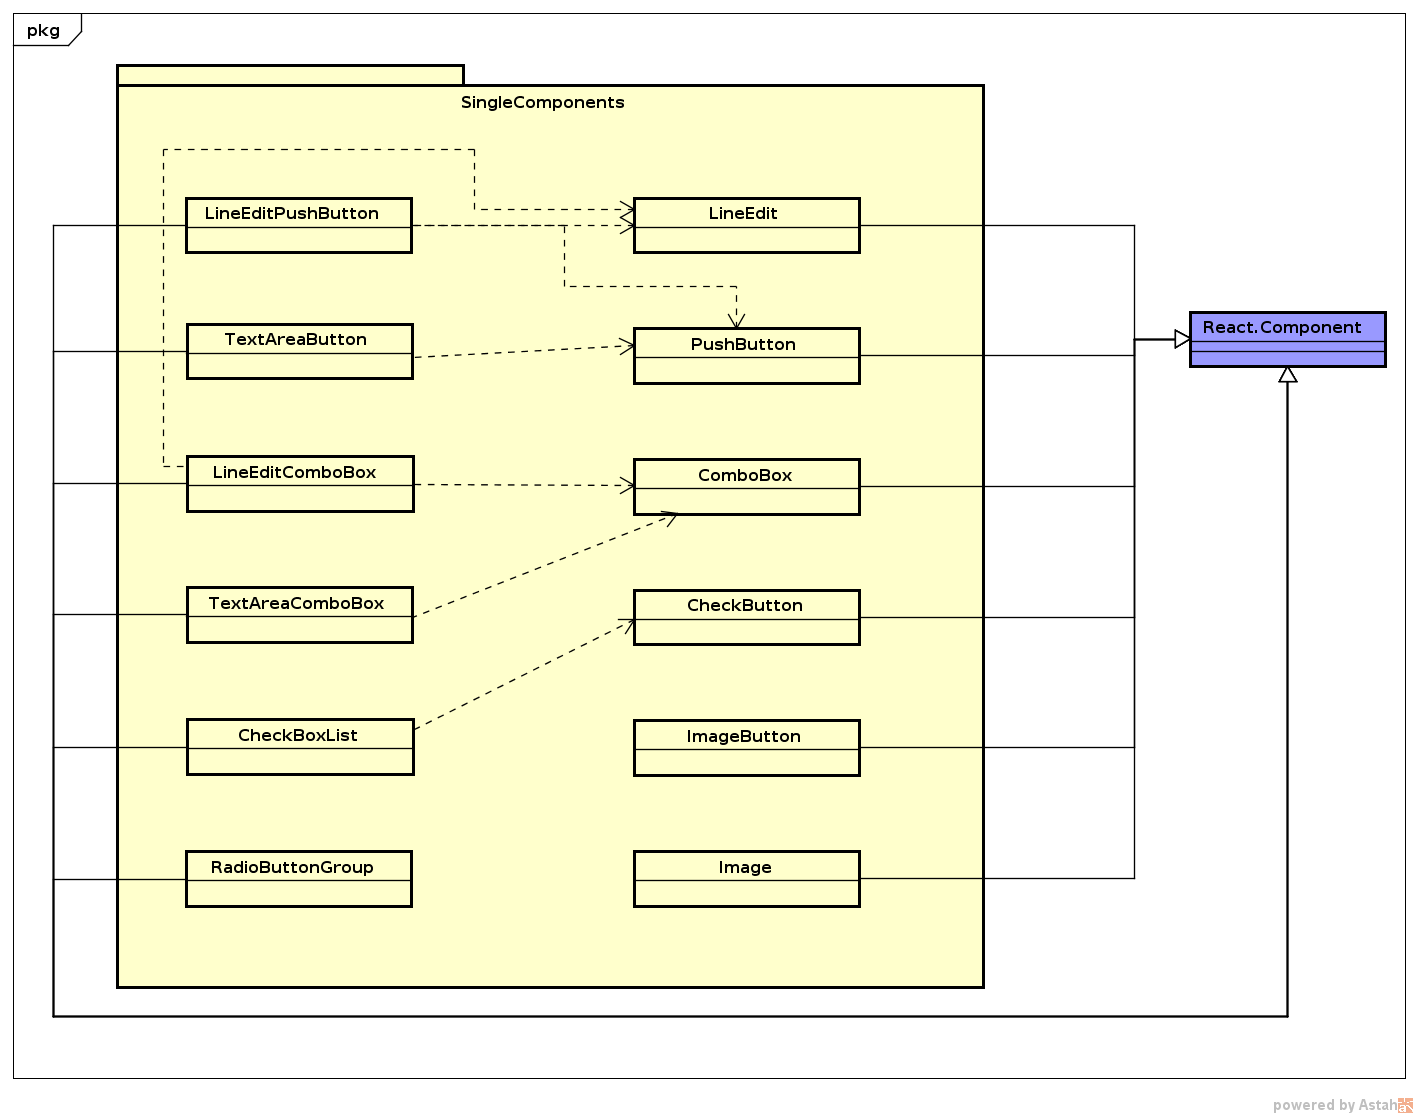
\includegraphics[width=\textwidth,keepaspectratio]{img/UI-SingleComponents}
   \caption{Diagramma per Monolith::UI::SingleComponents.}
\end{figure}
\FloatBarrier
\textbf{Descrizione}:\\
 Componente che contiene tutti i componenti React per la composizione della GUI 
\\ \textbf{Classi contenute}:\\
\begin{itemize}
\item CheckBoxList
\item CheckButton
\item ComboBox
\item Image
\item ImageButton
\item LineEdit
\item LineEditComboBox
\item LineEditPushButton
\item PushButton
\item RadioButtonGroup
\item TextAreaButton
\item TextAreaComboBox
\end{itemize}


\clearpage

\subsubsection{Monolith::UI::uiConstruction}
   \FloatBarrier
 %  \begin{sidewaysfigure}[ht]
%\begin{center}
 \makebox[\textwidth][c]{
\rotatebox{90}{
% \centering
\begin{minipage}{0.8\textheight}
   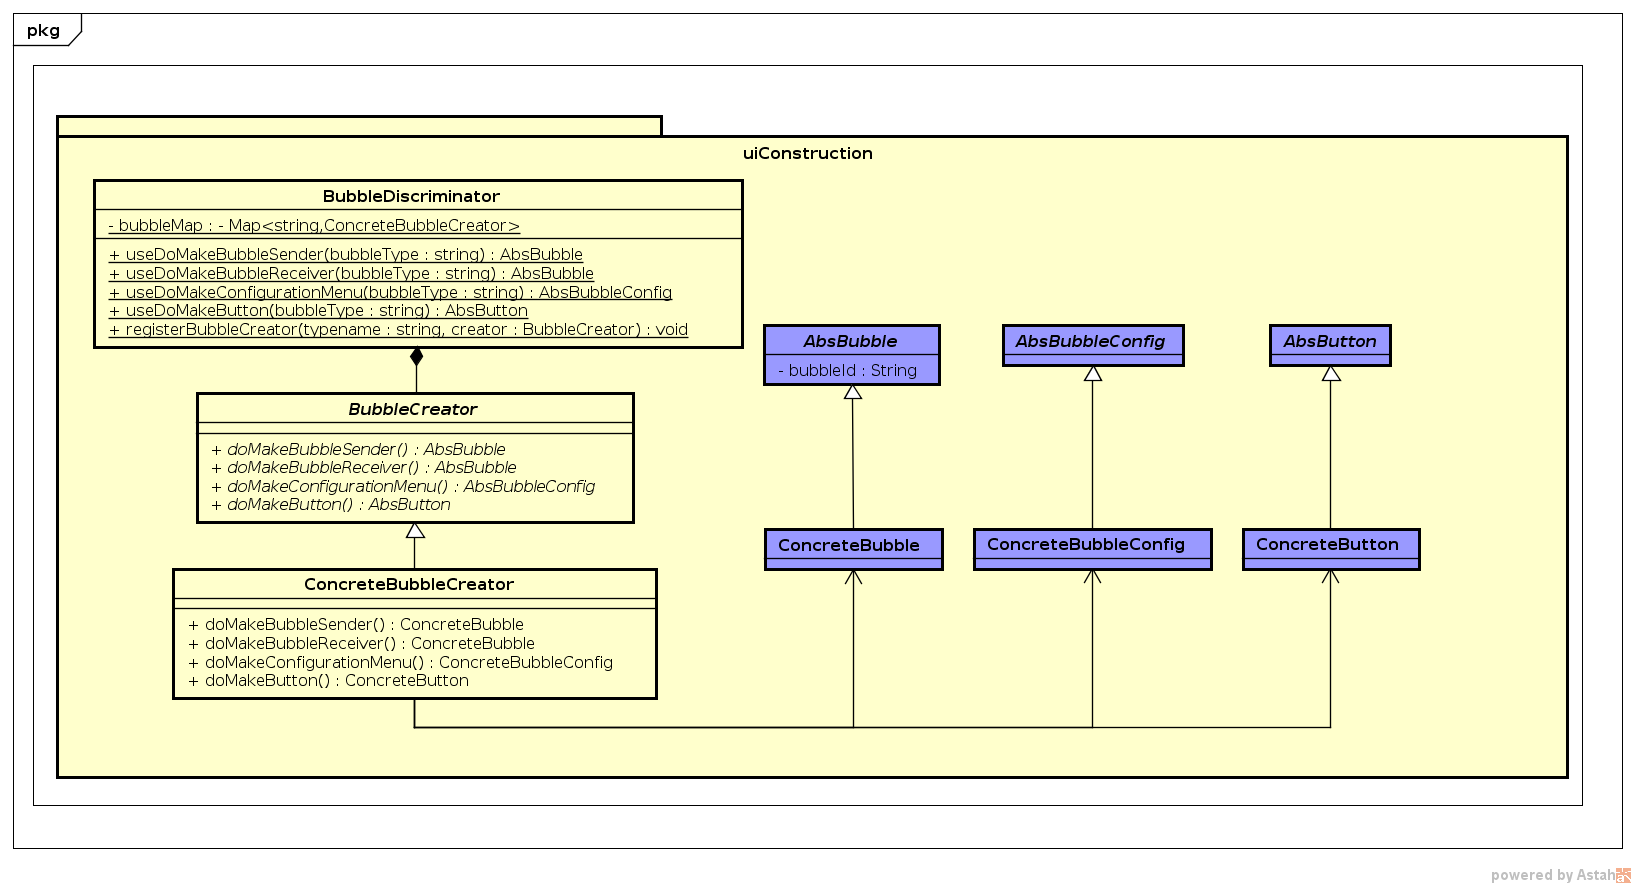
\includegraphics[width=\textwidth,keepaspectratio]{img/uiConstr}
  \captionof{figure}{Diagramma per Monolith::UI::uiConstruction.}
\end{minipage}}
}
%\end{center}
%\end{sidewaysfigure}
\FloatBarrier
\textbf{Descrizione}:\\
 Componente per la creazione delle bolle da visualizzare 
\\ \textbf{Classi contenute}:\\
\begin{itemize}
\item AbsBubble
\item AbsBubbleConfig
\item AbsButton
\item bubbleCreator
\item bubbleDiscriminator
\end{itemize}


\clearpage \subsection{Architettura generale - Bolle Demo}
\subsubsection{CurrencyBubble}
   \FloatBarrier
 %  \begin{sidewaysfigure}[ht]
%\begin{center}
 \makebox[\textwidth][c]{
\rotatebox{90}{
% \centering
\begin{minipage}{0.8\textheight}
   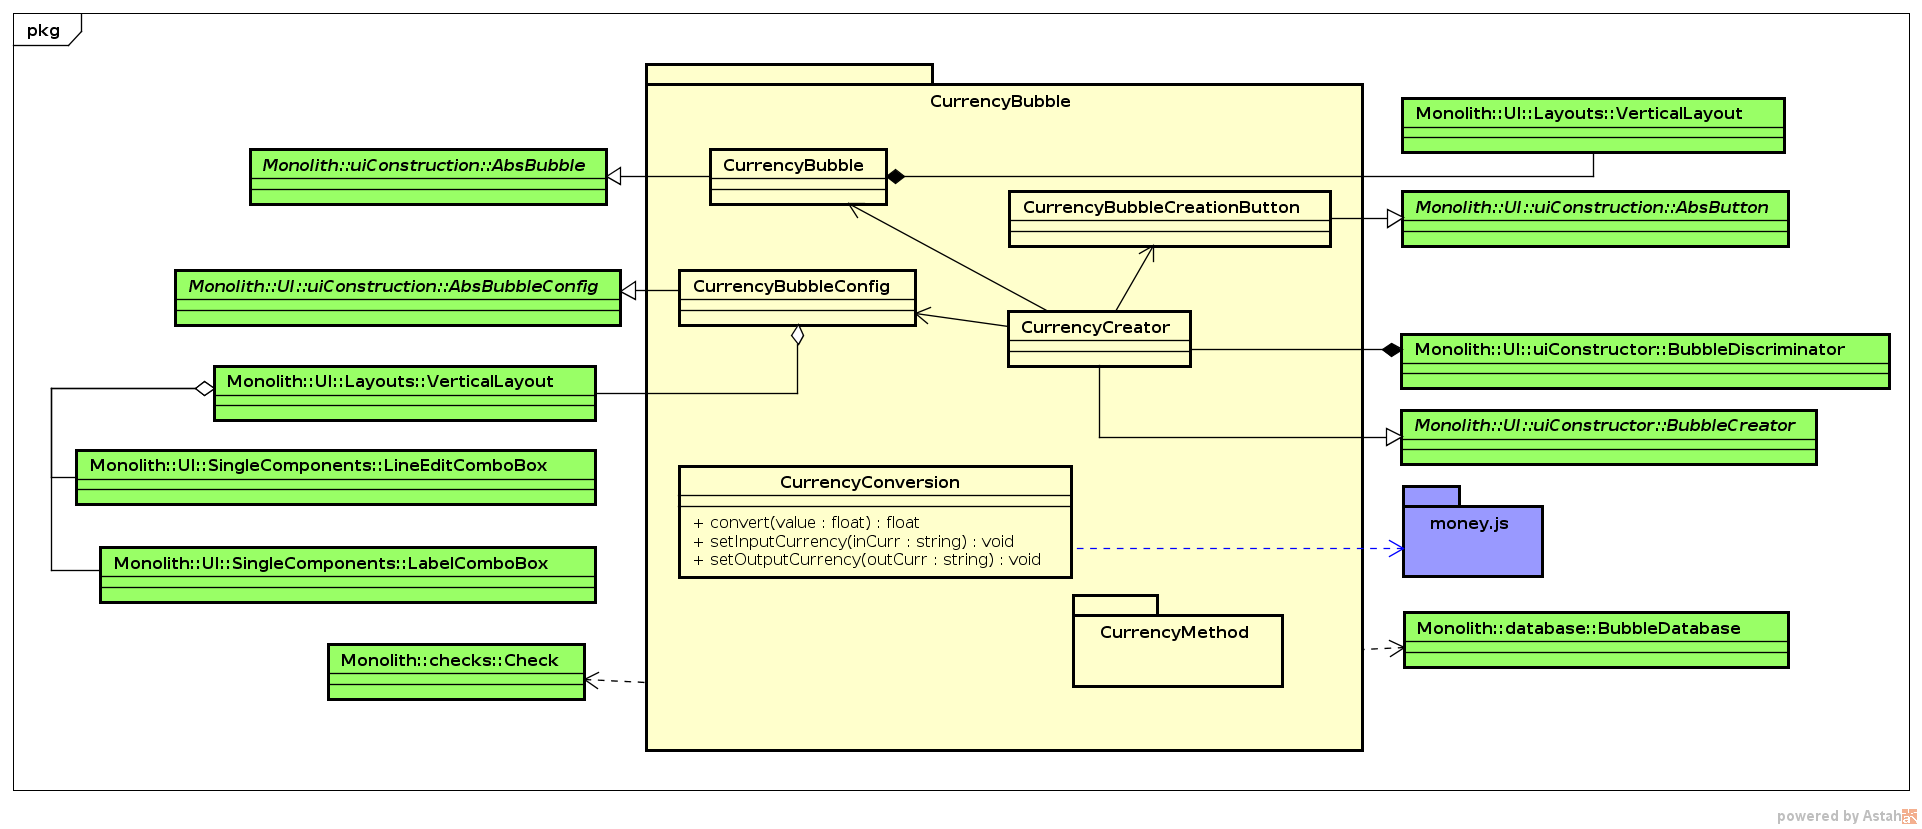
\includegraphics[width=\textwidth,keepaspectratio]{img/currency}
  \captionof{figure}{Diagramma per CurrencyBubble.}
\end{minipage}}
}
%\end{center}
%\end{sidewaysfigure}
\FloatBarrier
\textbf{Descrizione}:\\
 Componente contente le classi necessarie per la creazione della bolla convertitore valute. 
\\ \textbf{Classi contenute}:\\
\begin{itemize}
\item CurrencyBubble
\item CurrencyBubbleConfig
\item CurrencyBubbleCreationButton
\item CurrencyCreator
\end{itemize}


\clearpage

\subsubsection{CurrencyBubble::CurrencyMethod}
\textbf{Descrizione}:\\
 Componente che contiene la definizione dei Meteor.methods per le operazioni lato server della bolla currency.  In particolare BubbleCurrencyConvertor viene invocato dal metodo di inserimento di una nuova bolla per eseguire la conversione di valuta modificando l'oggetto inviato dal client prima dell'inserimento nel database. Utilizza la libreria request per scaricare da openexchangerates.org i dati di cui ha bisogno. Poi utilizza money.js per effettuare la conversione vera e propria. Ritorna poi l'oggetto modificato, pronto per essere inserito nel database. 


\clearpage

\subsubsection{ListBubble}
\textbf{Descrizione}:\\
 Componente contenente i pacchetti necessari per la creazione della bolla lista. 


\clearpage

\subsubsection{ListBubble::CheckListCreation}
\textbf{Descrizione}:\\
 Componente che si occupa della creazione delle check list. 
\\ \textbf{Classi contenute}:\\
\begin{itemize}
\item ListBubbleConfig
\item ListBubbleCreationButton
\end{itemize}


\clearpage

\subsubsection{ListBubble::CheckListReading}
\textbf{Descrizione}:\\
 Componente che si occupa della lettura e dell'utilizzo delle check list. 
\\ \textbf{Classi contenute}:\\
\begin{itemize}
\item ListBubble
\end{itemize}


\clearpage

\subsubsection{ListBubble::Configuration}
\textbf{Descrizione}:\\
 Componente che gestisce l'area di configurazione della bolla e il pulsante apposito da inserire nel menu iniziale di creazione. 


\clearpage

\subsubsection{ListBubble::DataManagement}
\textbf{Descrizione}:\\
 Componente che si occupa di tutte le operazioni di gestione dei dati che non sono gestite da Monolith. Usa il database MongoDB. 
\\ \textbf{Classi contenute}:\\
\begin{itemize}
\item ListBubbleCreator
\end{itemize}


\clearpage

\subsubsection{ListBubble::Receiver}
\textbf{Descrizione}:\\
 Componente che gestisce la visualizzazione della bolla da parte del ricevente. 


\clearpage

\subsubsection{ListBubble::Sender}
\textbf{Descrizione}:\\
 Componente che gestisce la visualizzazione della bolla da parte del mittente. 


\clearpage

\subsubsection{PollBubble}
   \FloatBarrier
 %  \begin{sidewaysfigure}[ht]
%\begin{center}
 \makebox[\textwidth][c]{
\rotatebox{90}{
% \centering
\begin{minipage}{0.8\textheight}
   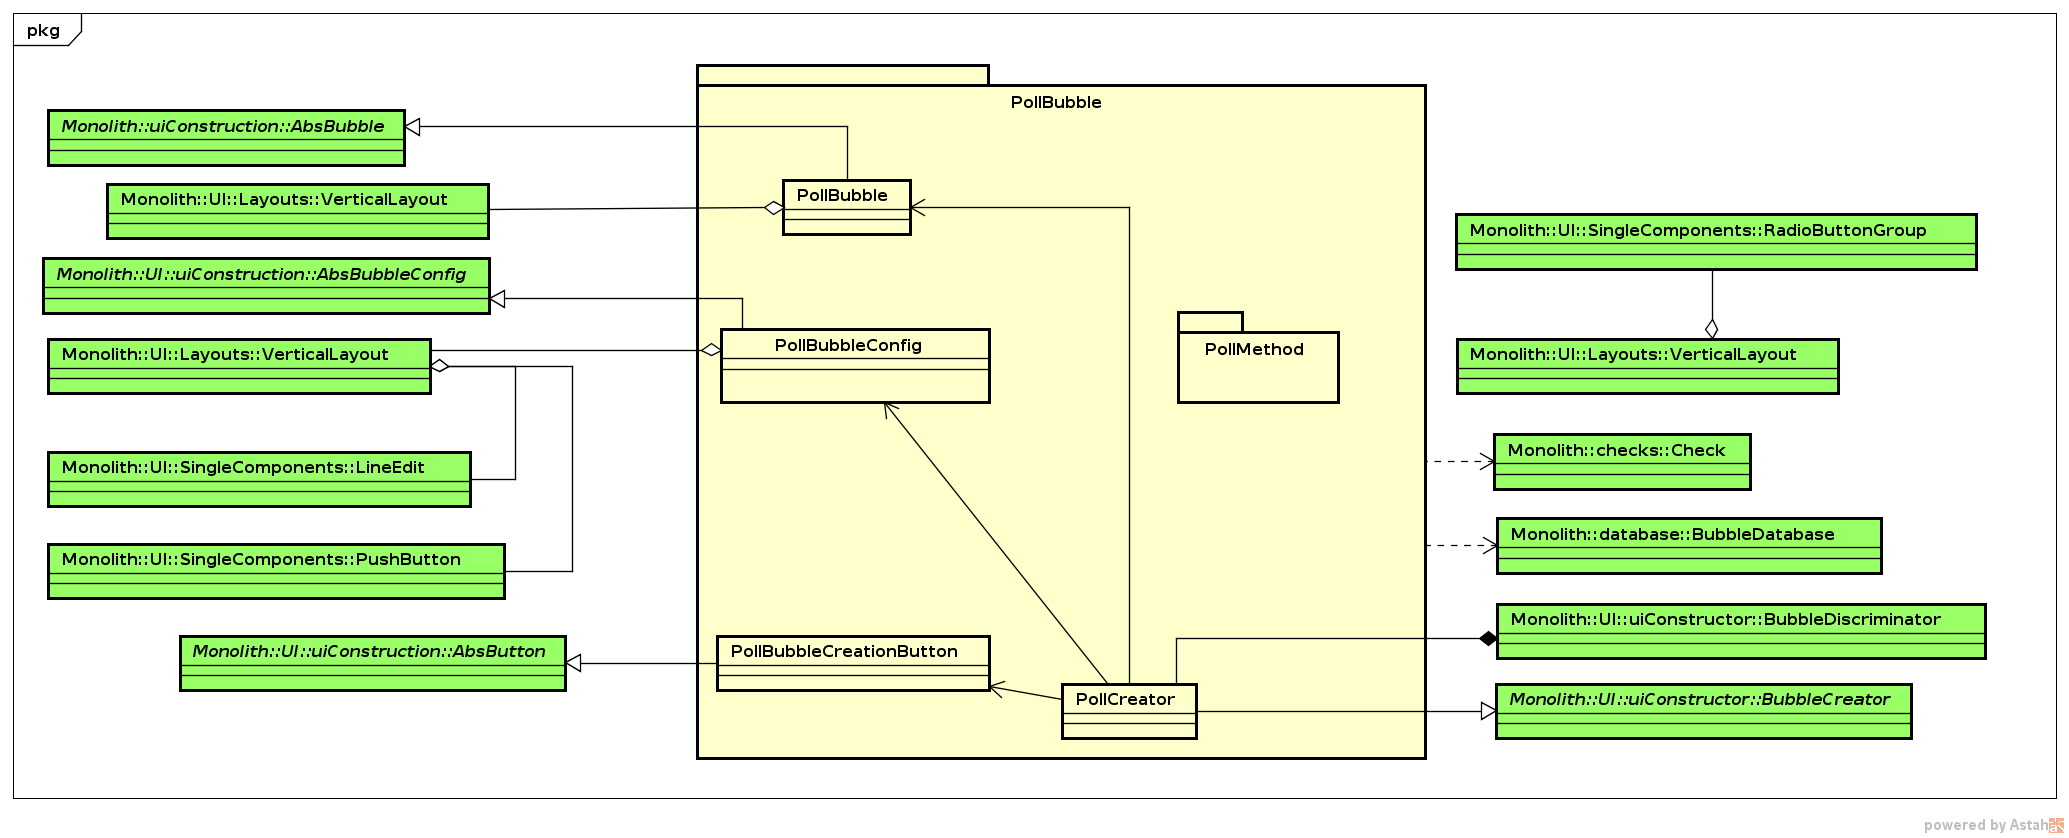
\includegraphics[width=\textwidth,keepaspectratio]{img/poll}
  \captionof{figure}{Diagramma per PollBubble.}
\end{minipage}}
}
%\end{center}
%\end{sidewaysfigure}
\FloatBarrier
\textbf{Descrizione}:\\
 Componente contente le classi necessarie per la creazione della bolla sondaggio. 
\\ \textbf{Classi contenute}:\\
\begin{itemize}
\item PollBubble
\item PollBubbleConfig
\item PollBubbleCreationButton
\item PollCreator
\end{itemize}


\clearpage

\subsubsection{PollBubble::PollMethod}
\textbf{Descrizione}:\\
 Componente che contiene la definizione dei Meteor.methods per le operazioni lato server della bolla poll,  In particolare BubblePollUpdate viene invocato dal metodo di aggiornamento di una bolla per incrementare il contatore dei voti. Utilizza direttamente l'accesso alla collezione su MongoDb 


\clearpage

\subsubsection{RandomBubble}
   \FloatBarrier
 %  \begin{sidewaysfigure}[ht]
%\begin{center}
 \makebox[\textwidth][c]{
\rotatebox{90}{
% \centering
\begin{minipage}{0.8\textheight}
   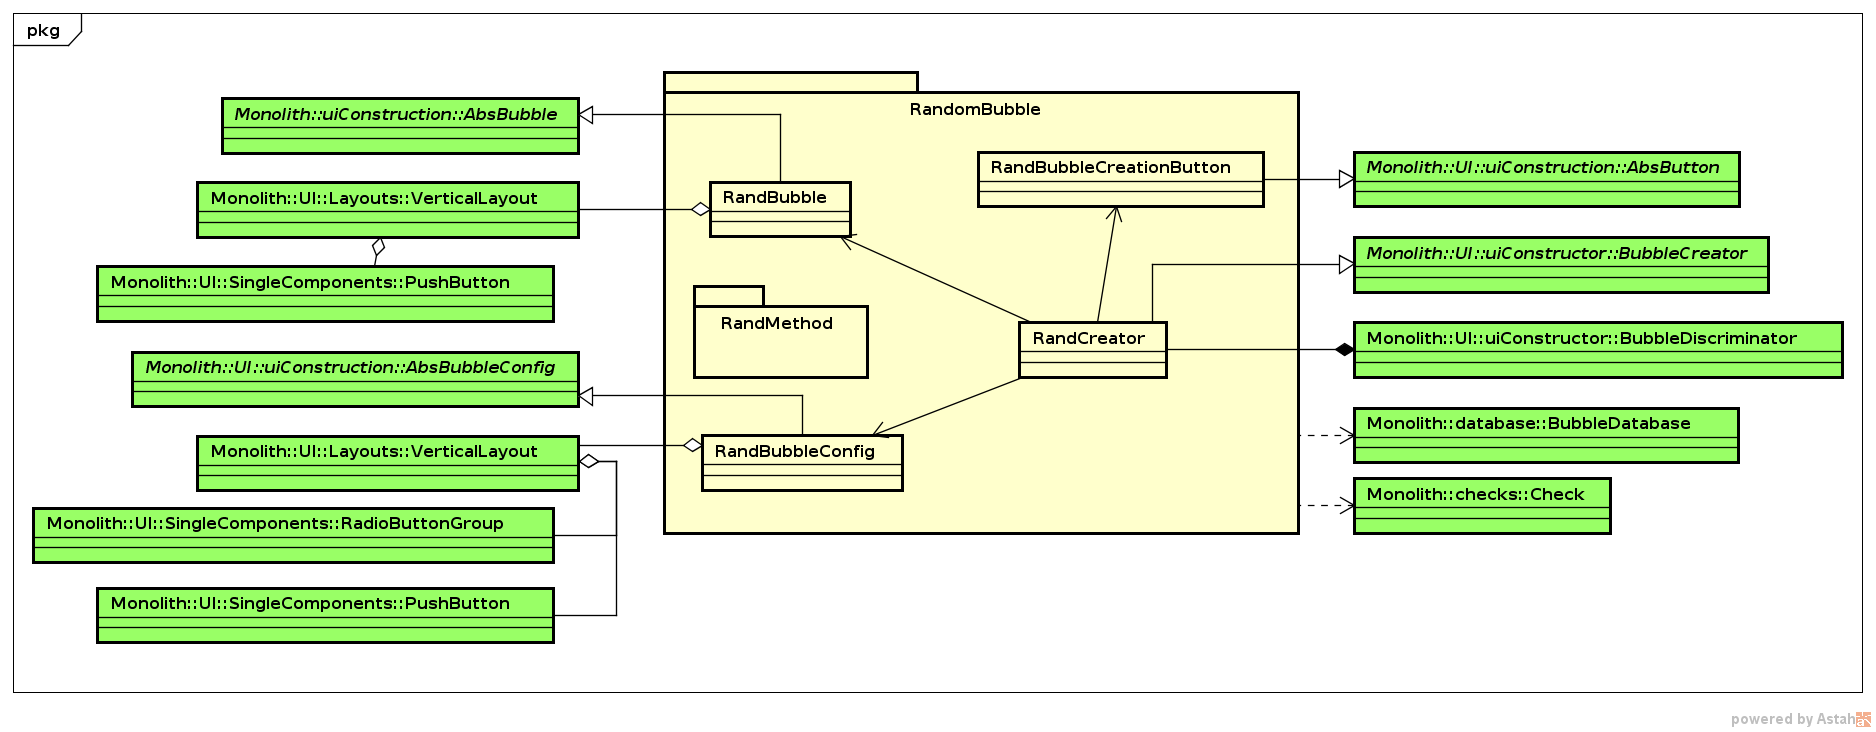
\includegraphics[width=\textwidth,keepaspectratio]{img/random}
  \captionof{figure}{Diagramma per RandomBubble.}
\end{minipage}}
}
%\end{center}
%\end{sidewaysfigure}
\FloatBarrier
\textbf{Descrizione}:\\
 Componente contente le classi necessarie per la creazione della bolla estrazione numero casuale. 
\\ \textbf{Classi contenute}:\\
\begin{itemize}
\item RandBubble
\item RandBubbleConfig
\item RandBubbleCreationButton
\item RandCreator
\end{itemize}


\clearpage

\subsubsection{RandomBubble::RandMethod}
\textbf{Descrizione}:\\
 Componente che contiene la definizione dei Meteor.methods per le operazioni lato server della bolla random.  In particolare:
\\begin{itemize}
\\item BubbleRandomInsert viene invocato dal metodo di inserimento di una nuova bolla per eseguire l'estrazione del numero casuale da inserire nel database.
\\item  BubbleRandomUpdate effettua un'operazione analoga a quella di BubbleRandomInsert ma per le operazioni di update.
\\end{itemize} 





\clearpage

\subsection{Architettura di dettaglio - Classi del sistema Monolith}\subsubsection{Check}
\textbf{Componente:}  Monolith::checks\\
   \FloatBarrier
   \begin{figure}[ht]
   \centering
   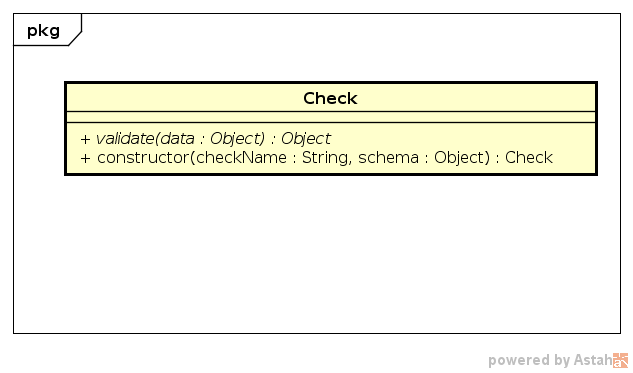
\includegraphics[width=0.6\textwidth]{img/single-Check}
   \caption{{Diagramma per Check in checks}}
\end{figure}
\FloatBarrier
\textbf{Descrizione}\\
Classe che rappresenta i controlli da eseguire lato server sull'input dell'utente. 
\begin{itemize}
\item +constructor(checkName: String, schema: Object) \\
Il costruttore riceve il nome con cui verrà registrato il controllo da eseguire e la descrizione dello schema dei dati. Il secondo argomento viene utilizzato per inizializzare un oggetto SimpleSchema.
\item +validate(dataObj:Object):boolean \\
Viene controllato che l'oggetto fornito come argomento corrisponda allo schema.
\end{itemize} 


\textbf{Applicazioni}\\
Prima di ogni inserimento sul database i dati vengono verificati utilizzando questa classe. 


\clearpage

\subsubsection{CheckHandler}
\textbf{Componente:}  Monolith::checks\\
   \FloatBarrier
   \begin{figure}[ht]
   \centering
   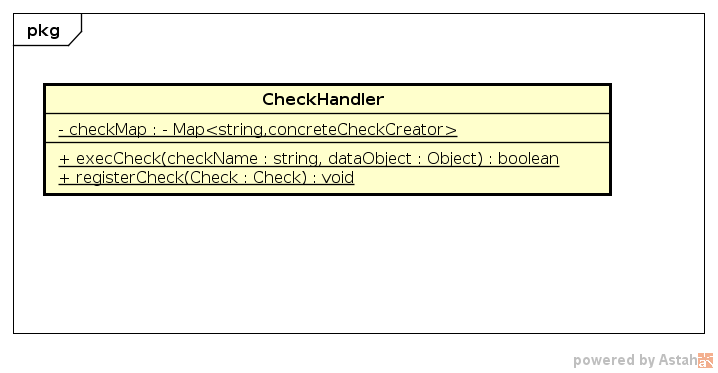
\includegraphics[width=0.6\textwidth]{img/single-CheckHandler}
   \caption{{Diagramma per CheckHandler in checks}}
\end{figure}
\FloatBarrier
\textbf{Descrizione}\\
Classe che contiene una mappa statica che associa i controlli (classe check) alle stringhe che li descrivono. 
\begin{itemize}
\item +registerCheck(check: Check) \\
Inserisce un check nella mappa
\item +execCheck(checkName:String, dataObj: Object):boolean \\
Esegue il check con il nome checkName sull'oggetto dataObj e ritorna un booleano che descrive la conformità dei dati. In caso il check non sia presente nella mappa allora viene lanciato un errore.
\end{itemize} 


\textbf{Applicazioni}\\
Viene utilizzato per eseguire i controlli sull'input lato server 


\clearpage

\subsubsection{BubbleDatabase}
\textbf{Componente:}  Monolith::Database\\
   \FloatBarrier
   \begin{figure}[ht]
   \centering
   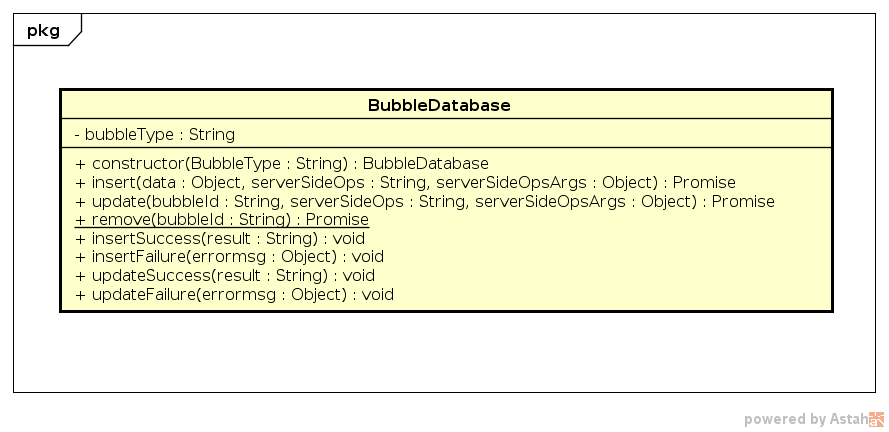
\includegraphics[width=0.6\textwidth]{img/single-BubbleDatabase}
   \caption{{Diagramma per BubbleDatabase in Database}}
\end{figure}
\FloatBarrier
\textbf{Descrizione}\\
Classe che fornisce un'interfaccia per utilizzare il database lato client. 
\\
Il costruttore chiede una stringa corrispondente al nome della bolla. Per ogni bolla si dovrà istanziare BubbleDatabase con il nome corrispondente.
\\
Ciascuno dei seguenti metodi ritorna una promise:
\begin{itemize} 
\item +insert(data: Object, serverSideOps, serverSideOpsArg) \\
Richiama il Meteor.Method insertBubble fornendo automaticamente alcuni parametri necessari e specificando la funzione lato server da eseguire sul database. 
\item +update(bubbleId, serverSideOps, serverSideOpsArgs) \\
Richiama il Meteor.Method updateBubble specificando la funzione lato server da eseguire sul database.
\item +remove(bubbleId) \\
Metodo statico che richiama il Meteor.method per rimuovere la bolla con l'id passato come agomento
\end{itemize}
I restanti metodi (insertSuccess, insertFailure, updateSuccess, updateFailure) vengono invocati automaticamente al successo o al fallimento di una delle operazioni sopra descritte e semplicemente stampano un messaggio sulla console. In caso di necessità possono essere ridefinite derivando la classe. 


\textbf{Applicazioni}\\
 


\clearpage

\subsubsection{SideArea1}
\textbf{Componente:}  Monolith::SideAreas::SideArea1\_pkg\\
   \FloatBarrier
   \begin{figure}[ht]
   \centering
   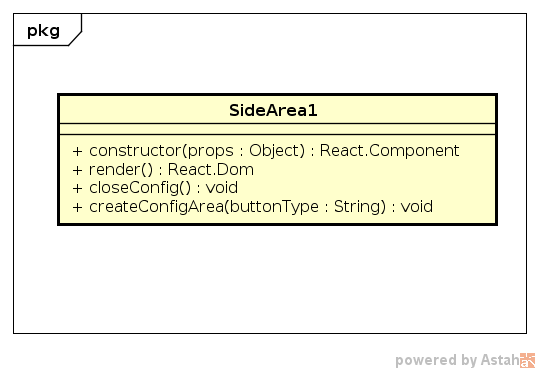
\includegraphics[width=0.6\textwidth]{img/single-SideArea1}
   \caption{{Diagramma per SideArea1 in SideArea1\_pkg}}
\end{figure}
\FloatBarrier
\textbf{Descrizione}\\
Classe che rappresenta il componente React per la visualizzazione del contenuto della prima area laterale. \ 
\textbf{Metodi:}
\begin{itemize}

\item +constructor(props : Object) : React.Component 
\\
Costruttore della sottoclasse di React.Component in cui è necessario chiamare super (props) ed è possibile inizializzare lo stato per i dati soggetti a cambiamento.

\item +render() : React.DOM 
\\
Metodo che esamina this.props e this.state e restituisce un componente che funga da contenitore per la prima area laterale.

\end{itemize} 


\textbf{Applicazioni}\\
Viene utilizzata all'apertura della prima area laterale per visualizzare il menù di creazione delle bolle e lo storico delle bolle inviate. 


\clearpage

\subsubsection{BubbleMenu}
\textbf{Componente:}  Monolith::SideAreas::SideArea1\_pkg\\
   \FloatBarrier
   \begin{figure}[ht]
   \centering
   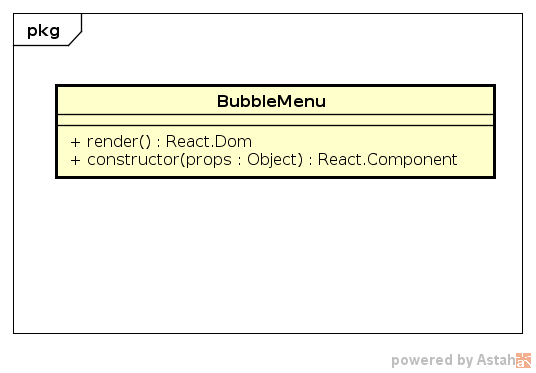
\includegraphics[width=0.6\textwidth]{img/single-BubbleMenu}
   \caption{{Diagramma per BubbleMenu in SideArea1\_pkg}}
\end{figure}
\FloatBarrier
\textbf{Descrizione}\\
Classe che contiene i pulsanti che portano alla configurazione delle singole bolle.
\textbf{Metodi:} 
\begin{itemize}
\item +constructor(props : Object) : React.Component 
\\
Costruttore della sottoclasse di React.Component in cui è necessario chiamare super (props) ed è possibile inizializzare lo stato per i dati soggetti a cambiamento.
\item +render() : React.DOM 
\\
Metodo che esamina this.props e this.state e restituisce un singolo elemento React che può essere una rappresentazione di un componente DOM nativo o un altro componente composito.
\end{itemize} 


\textbf{Applicazioni}\\
Viene utilizzata dalla SideArea1 per la visualizzazione del menù contenente i pulsanti per la creazione delle bolle. 


\clearpage

\subsubsection{ConfigArea}
\textbf{Componente:}  Monolith::SideAreas::SideArea1\_pkg\\
   \FloatBarrier
   \begin{figure}[ht]
   \centering
   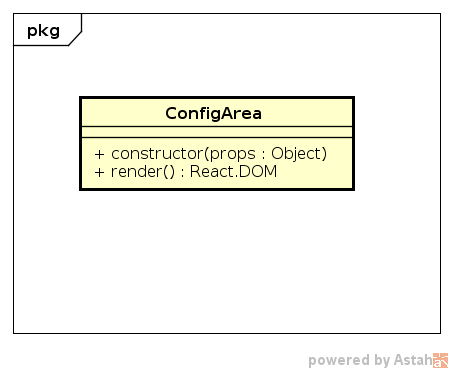
\includegraphics[width=0.6\textwidth]{img/single-ConfigArea}
   \caption{{Diagramma per ConfigArea in SideArea1\_pkg}}
\end{figure}
\FloatBarrier
\textbf{Descrizione}\\
Componente React in cui la SideArea1 inserisce i componenti grafici di configurazione. Questi possono essere i menu di configurazione per le bolle o altri menu di impostazioni 


\textbf{Applicazioni}\\
Viene utilizzato da SideArea1 per mostrare componenti grafici a scomparsa 


\clearpage

\subsubsection{SentBubbles}
\textbf{Componente:}  Monolith::SideAreas::SideArea1\_pkg\\
   \FloatBarrier
   \begin{figure}[ht]
   \centering
   \includegraphics[width=0.6\textwidth]{img/single-SentBubbles}
   \caption{{Diagramma per SentBubbles in SideArea1\_pkg}}
\end{figure}
\FloatBarrier
\textbf{Descrizione}\\
Classe che rappresenta il componente React per la visualizzazione dello storico delle bolle inviate.

\textbf{Metodi:} 
\begin{itemize}

\item +constructor(props : Object) : React.Component 
\\
Costruttore della sottoclasse di React.Component in cui è necessario chiamare super (props) ed è possibile inizializzare lo stato per i dati soggetti a cambiamento.

\item +render() : React.DOM 
\\
Metodo che esamina this.props e this.state e restituisce un componente che raccolga lo storico delle bolle inviate.

\end{itemize} 


\textbf{Applicazioni}\\
Viene utilizzata dalla SideArea1 per la visualizzazione dello storico delle bolle inviate. 


\clearpage

\subsubsection{SideArea2}
\textbf{Componente:}  Monolith::SideAreas::SideArea2\_pkg\\
   \FloatBarrier
   \begin{figure}[ht]
   \centering
   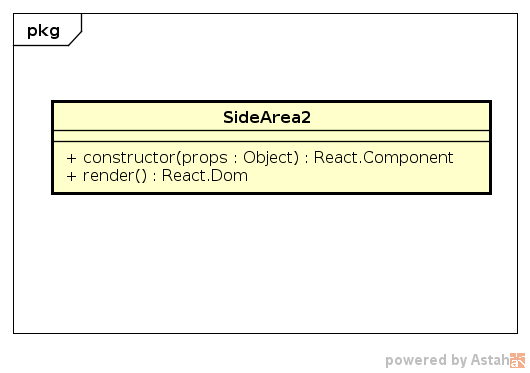
\includegraphics[width=0.6\textwidth]{img/single-SideArea2}
   \caption{{Diagramma per SideArea2 in SideArea2\_pkg}}
\end{figure}
\FloatBarrier
\textbf{Descrizione}\\
Classe che rappresenta il componente React per la visualizzazione del contenuto della seconda area laterale. \\
\textbf{Metodi:} 
\begin{itemize}

\item +constructor(props : Object) : React.Component 
\\
Costruttore della sottoclasse di React.Component in cui è necessario chiamare super (props) ed è possibile inizializzare lo stato per i dati soggetti a cambiamento.

\item +render() : React.DOM 
\\
Metodo che esamina this.props e this.state e restituisce un componente che funge da contenitore per la seconda area laterale.

\end{itemize} 


\textbf{Applicazioni}\\
Viene utilizzata all'apertura della seconda area laterale per visualizzare dello storico delle bolle ricevute. 


\clearpage

\subsubsection{ReceivedBubble}
\textbf{Componente:}  Monolith::SideAreas::SideArea2\_pkg\\
   \FloatBarrier
   \begin{figure}[ht]
   \centering
   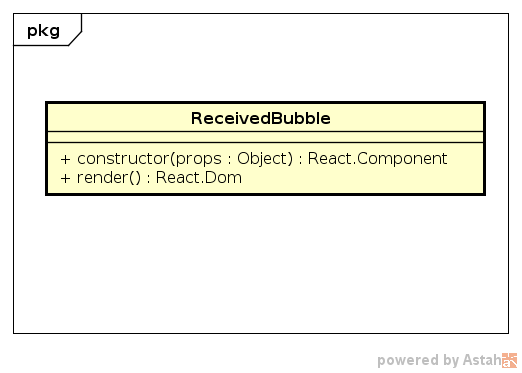
\includegraphics[width=0.6\textwidth]{img/single-ReceivedBubble}
   \caption{{Diagramma per ReceivedBubble in SideArea2\_pkg}}
\end{figure}
\FloatBarrier
\textbf{Descrizione}\\
Classe che rappresenta il componente React per la visualizzazione dello storico delle bolle ricevute. \\
\textbf{Metodi:} 
\begin{itemize}
\item +constructor(props : Object) : React.Component 
\\
Costruttore della sottoclasse di React.Component in cui è necessario chiamare super (props) ed è possibile inizializzare lo stato per i dati soggetti a cambiamento.
\item +render() : React.DOM 
\\
Metodo che esamina this.props e this.state e restituisce un singolo elemento React che può essere una rappresentazione di un componente DOM nativo o un altro componente composito.
\end{itemize} 


\textbf{Applicazioni}\\
Viene utilizzata dalla SideArea2 per la visualizzazione dello storico delle bolle ricevute. 


\clearpage

\subsubsection{VerticalLayout}
\textbf{Componente:}  Monolith::UI::Layouts\\
   \FloatBarrier
   \begin{figure}[ht]
   \centering
   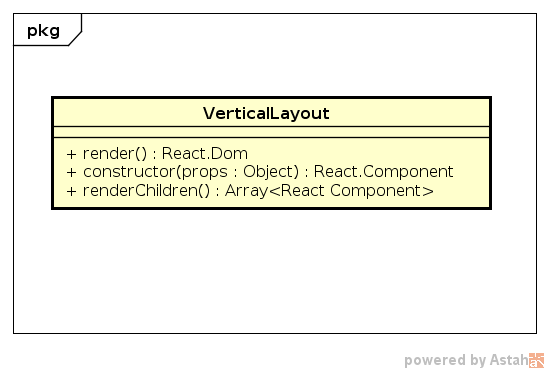
\includegraphics[width=0.6\textwidth]{img/single-VerticalLayout}
   \caption{{Diagramma per VerticalLayout in Layouts}}
\end{figure}
\FloatBarrier
\textbf{Descrizione}\\
Classe contenitore che dispone i componenti contenuti in verticale. \\
\textbf{Metodi:}
\begin{itemize}

\item +constructor(props : Object) : React.Component 
\\
Costruttore della sottoclasse di React.Component in cui è necessario chiamare super (props) ed è possibile inizializzare lo stato per i dati soggetti a cambiamento.

\item +render() : React.DOM 
\\
Metodo che esamina this.props e this.state e restituisce un contenitore di elementi che li dispone in verticale.

\item +countMyChildren() : int
\\
Metodo che ritorna un intero contente il numero di componenti figli, utilizzato per impostare la classe bootstrap corretta.

\end{itemize} 


\textbf{Applicazioni}\\
Utilizzata per assegnare l'attributo className bootstrap a tutti i componenti figli, in modo che vengano visualizzati allineati in verticale con la dimensione adeguata. 


\clearpage

\subsubsection{ContainedElement}
\textbf{Componente:}  Monolith::UI::Layouts\\
   \FloatBarrier
   \begin{figure}[ht]
   \centering
   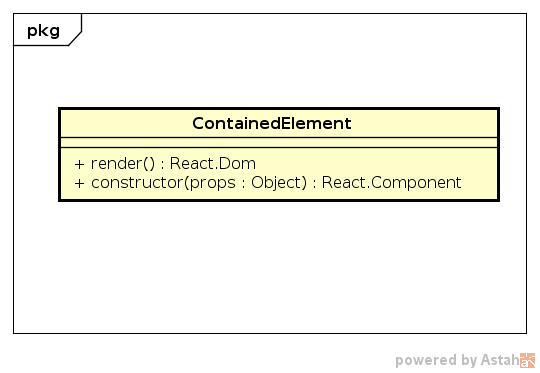
\includegraphics[width=0.6\textwidth]{img/single-ContainedElement}
   \caption{{Diagramma per ContainedElement in Layouts}}
\end{figure}
\FloatBarrier
\textbf{Descrizione}\\
Classe che rappresenta il layout di un contenitore generico. \\
\textbf{Metodi:} 
\begin{itemize}

\item +constructor(props : Object) : React.Component 
\\
Costruttore della sottoclasse di React.Component in cui è necessario chiamare super (props) ed è possibile inizializzare lo stato per i dati soggetti a cambiamento.

\item +render() : React.DOM 
\\
Metodo che esamina this.props e this.state e restituisce un elemento "div" contenenti i figli ed utilizzando lo stile CSS passato nella props "classNames".

\end{itemize} 


\textbf{Applicazioni}\\
Viene utilizzata dalle classi HorizontalLayout, VerticalLayout e ConditionalRendering per contenere un componente generico 


\clearpage

\subsubsection{HorizontalLayout}
\textbf{Componente:}  Monolith::UI::Layouts\\
   \FloatBarrier
   \begin{figure}[ht]
   \centering
   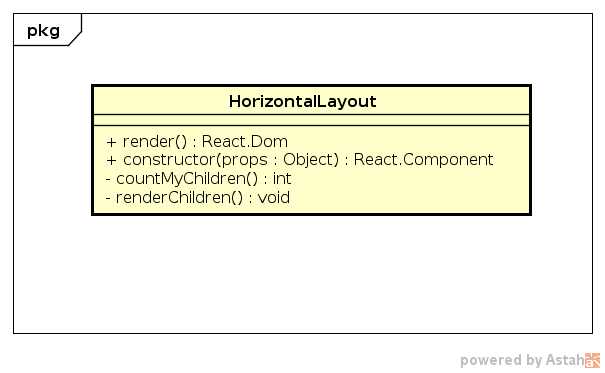
\includegraphics[width=0.6\textwidth]{img/single-HorizontalLayout}
   \caption{{Diagramma per HorizontalLayout in Layouts}}
\end{figure}
\FloatBarrier
\textbf{Descrizione}\\
Classe contenitore che dispone i componenti contenuti in orizzontale. \\
\textbf{Metodi:}
\begin{itemize}

\item +constructor(props : Object) : React.Component 
\\
Costruttore della sottoclasse di React.Component in cui è necessario chiamare super (props) ed è possibile inizializzare lo stato per i dati soggetti a cambiamento.

\item +render() : React.DOM 
\\
Metodo che esamina this.props e this.state e restituisce un contenitore di elementi che li dispone in orizzontale.

\item +countMyChildren() : int \\
Metodo che ritorna un intero contente il numero di componenti figli, utilizzato per impostare la classe bootstrap corretta.

\end{itemize} 


\textbf{Applicazioni}\\
Utilizzata per assegnare l'attributo className bootstrap a tutti i componenti figli, in modo che vengano visualizzati allineati in orizzontale con la dimensione adeguata. 


\clearpage

\subsubsection{Image}
\textbf{Componente:}  Monolith::UI::SingleComponents\\
   \FloatBarrier
   \begin{figure}[ht]
   \centering
   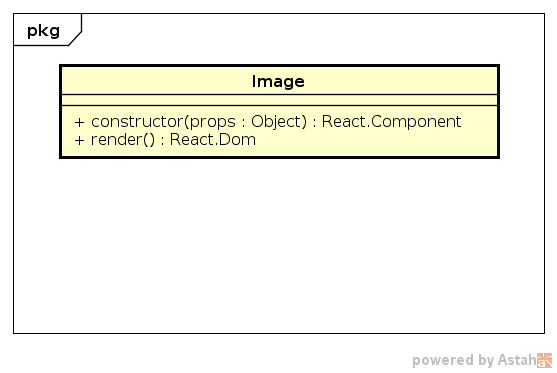
\includegraphics[width=0.6\textwidth]{img/single-Image}
   \caption{{Diagramma per Image in SingleComponents}}
\end{figure}
\FloatBarrier
\textbf{Descrizione}\\
Componente React che rappresenta un'immagine. \\
\textbf{Metodi:} 
\begin{itemize}
\item +constructor(props : Object) : React.Component 
\\
Costruttore della sottoclasse di React.Component in cui è necessario chiamare super (props) ed è possibile inizializzare lo stato per i dati soggetti a cambiamento.
\item +render() : React.DOM 
\\
Metodo che esamina this.props e this.state e restituisce un immagine con le proprietà datele.
\end{itemize} 


\textbf{Applicazioni}\\
Viene utilizzato per rappresentare un immagine all'interno di una bolla.
Image può avere le seguenti props:
\begin{itemize}
\item classes:
\\
Stile CSS per il componente.
\item id:
\\
Un Id per il componente React.
\item src: 
\\
Come per tag HTML "img".
\item alt: 
\\
Come per tag HTML "img".
\item width: \\
Come per tag HTML "img".
\item height: \\
Come per tag HTML "img". 
\end{itemize}

\clearpage

\subsubsection{ComboBox}
\textbf{Componente:}  Monolith::UI::SingleComponents\\
   \FloatBarrier
   \begin{figure}[ht]
   \centering
   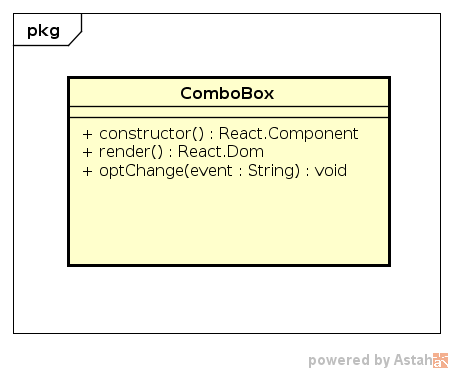
\includegraphics[width=0.6\textwidth]{img/single-ComboBox}
   \caption{{Diagramma per ComboBox in SingleComponents}}
\end{figure}
\FloatBarrier
\textbf{Descrizione}\\
Componente React che rappresenta un combobox. \\
\textbf{Metodi:} 
\begin{itemize}
\item +constructor(props : Object) : React.Component 
\\
Costruttore della sottoclasse di React.Component in cui è necessario chiamare super (props) ed è possibile inizializzare lo stato per i dati soggetti a cambiamento.

\item +optChange(event : String) : void  
\\
Comunica alla funzione "padre" l'opzione selezionata.

\item +render() : React.DOM 
\\
Metodo che esamina this.props e this.state e restituisce un singolo elemento combobox con le opzione passategli nelle props.

\end{itemize} 


\textbf{Applicazioni}\\
Componente React rappresentante una combobox e costruibile passando un array contenente le varie opzioni nella props "options". 


\clearpage

\subsubsection{LineEdit}
\textbf{Componente:}  Monolith::UI::SingleComponents\\
   \FloatBarrier
   \begin{figure}[ht]
   \centering
   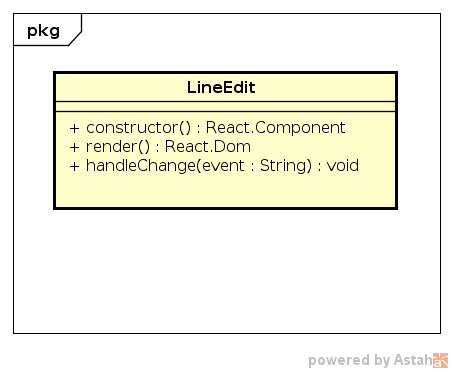
\includegraphics[width=0.6\textwidth]{img/single-LineEdit}
   \caption{{Diagramma per LineEdit in SingleComponents}}
\end{figure}
\FloatBarrier
\textbf{Descrizione}\\
Componente React che rappresenta un input di testo. \\
\textbf{Metodi:} 
\begin{itemize}
\item +constructor(props : Object) : React.Component 
\\
Costruttore della sottoclasse di React.Component in cui è necessario chiamare super (props) ed è possibile inizializzare lo stato per i dati soggetti a cambiamento.
\item +handleChange(event : String) : void  
\\
Comunica la stringa digitata al "padre". 
\item +render() : React.DOM 
\\
Metodo che esamina this.props e this.state e restituisce un singolo elemento React che rappresenta un input di testo.
\end{itemize} 


\textbf{Applicazioni}\\
Viene utilizzato per costruire eventuali interfacce grafiche delle bolle. \\
Si aspetta una props "id" per distinguere il componente. 


\clearpage

\subsubsection{PushButton}
\textbf{Componente:}  Monolith::UI::SingleComponents\\
   \FloatBarrier
   \begin{figure}[ht]
   \centering
   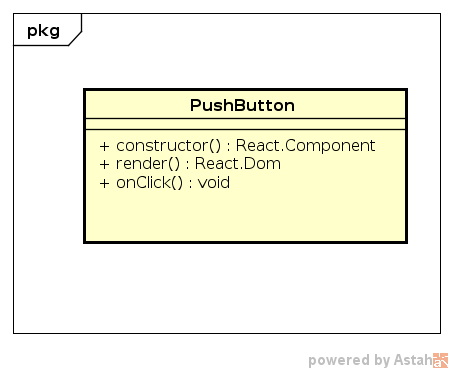
\includegraphics[width=0.6\textwidth]{img/single-PushButton}
   \caption{{Diagramma per PushButton in SingleComponents}}
\end{figure}
\FloatBarrier
\textbf{Descrizione}\\
Componente React che rappresenta un pulsante. \\
\textbf{Metodi:} 
\begin{itemize}
\item +constructor(props : Object) : React.Component 
\\
Costruttore della sottoclasse di React.Component in cui è necessario chiamare super (props) ed è possibile inizializzare lo stato per i dati soggetti a cambiamento.

\item +onClick(): void 
\ 
Viene passato al "padre" l'ID del pulsante cliccato.

\item +render() : React.DOM 
\\
Metodo che esamina this.props e this.state e restituisce un singolo elemento React che rappresenta un pulsante eventualmente cliccabile.

\end{itemize} 


\textbf{Applicazioni}\\
Componente React che rappresenta un pulsante che può essere cliccabile (o meno) in base all valore della props "dis". \ Questa può assumere valore \textit{true} o \textit{false}. 


\clearpage

\subsubsection{CheckButton}
\textbf{Componente:}  Monolith::UI::SingleComponents\\
   \FloatBarrier
   \begin{figure}[ht]
   \centering
   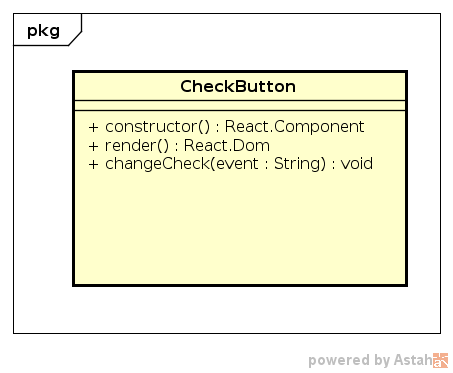
\includegraphics[width=0.6\textwidth]{img/single-CheckButton}
   \caption{{Diagramma per CheckButton in SingleComponents}}
\end{figure}
\FloatBarrier
\textbf{Descrizione}\\
Componente React che rappresenta un elemento di checkbox. \\
\textbf{Metodi:} 
\begin{itemize}

\item +constructor(props : Object) : React.Component 
\\
Costruttore della sottoclasse di React.Component in cui è necessario chiamare super (props) ed è possibile inizializzare lo stato per i dati soggetti a cambiamento.

\item +changeCheck(event : String) : void  
\\
Comunica l’opzione selezionata tramite il metodo del genitore. 

\item +render() : React.DOM 
\\
Metodo che esamina this.props e this.state e restituisce un singolo elemento React che può essere una rappresentazione di un componente DOM nativo o un altro componente composito.

\end{itemize} 


\textbf{Applicazioni}\\
Componente React che rappresenta un checkbox e contiene un metodo per comunicare al "padre" tutti i dati del oggetto quando questo viene cliccato. 


\clearpage

\subsubsection{ImageButton}
\textbf{Componente:}  Monolith::UI::SingleComponents\\
   \FloatBarrier
   \begin{figure}[ht]
   \centering
   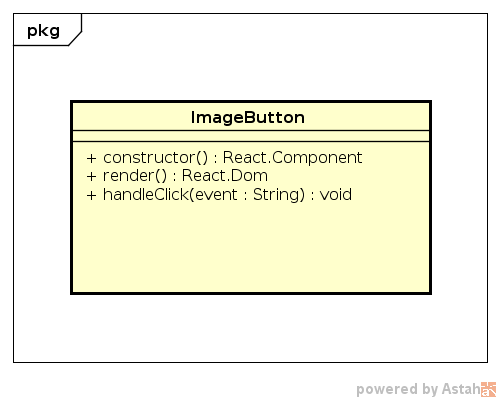
\includegraphics[width=0.6\textwidth]{img/single-ImageButton}
   \caption{{Diagramma per ImageButton in SingleComponents}}
\end{figure}
\FloatBarrier
\textbf{Descrizione}\\
Componente React che rappresenta un immagine che funge da pulsante. \\
\textbf{Metodi:} 
\begin{itemize}
\item +constructor(props : Object) : React.Component 
\\
Costruttore della sottoclasse di React.Component in cui è necessario chiamare super (props) ed è possibile inizializzare lo stato per i dati soggetti a cambiamento.
\item +handleClick() : void 
\\
Comunica l'Id dell'immagine cliccata al "padre". 
\item +render() : React.DOM 
\\
Metodo che esamina this.props e this.state e restituisce un singolo elemento React che rappresenta un'immagine cliccabile.
\end{itemize} 


\textbf{Applicazioni}\\
Componente React che rappresenta un'immagine cliccabile.\ Richiede le stesse props del componente "Image" con l'aggiunta di "handleClick" che comunica al "padre" l'id del componente cliccato. 


\clearpage

\subsubsection{CheckBoxList}
\textbf{Componente:}  Monolith::UI::SingleComponents\\
   \FloatBarrier
   \begin{figure}[ht]
   \centering
   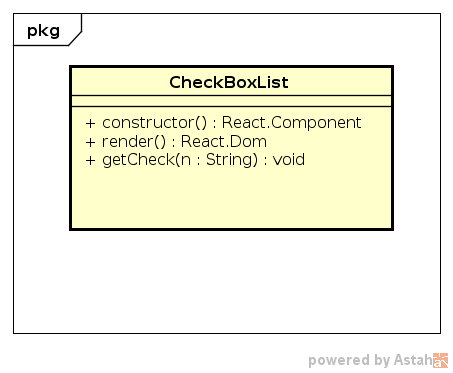
\includegraphics[width=0.6\textwidth]{img/single-CheckBoxList}
   \caption{{Diagramma per CheckBoxList in SingleComponents}}
\end{figure}
\FloatBarrier
\textbf{Descrizione}\\
Componente React che rappresenta una lista di CheckButton. \\
\textbf{Metodi:} 
\begin{itemize}
\item +constructor(props : Object) : React.Component 
\\
Costruttore della sottoclasse di React.Component in cui è necessario chiamare super (props) ed è possibile inizializzare lo stato per i dati soggetti a cambiamento.

\item +getCheck (n : Object) : void \\
Funzione che passa al "padre" i dati del CheckButton cliccato. 

\item +render() : React.DOM 
\\
Metodo che esamina this.props e this.state e restituisce un singolo elemento React che può essere una rappresentazione di un componente DOM nativo o un altro componente composito.

\end{itemize}
\\
\textbf{Props:} 
\begin{itemize}
\item options: 
\\
Passare un array di opzioni contenenti, per ciascuna di esse, un "id" ed un "value".
\item getCheck: 
\\
Passare una funzione che raccolga un oggetto di ritorno contenente i dati del CheckButton cliccato.

\end{itemize} 


\textbf{Applicazioni}\\
Componente React utile per costruire una lista di CheckButton passandogli un array di opzioni. 


\clearpage

\subsubsection{TextAreaButton}
\textbf{Componente:}  Monolith::UI::SingleComponents\\
   \FloatBarrier
   \begin{figure}[ht]
   \centering
   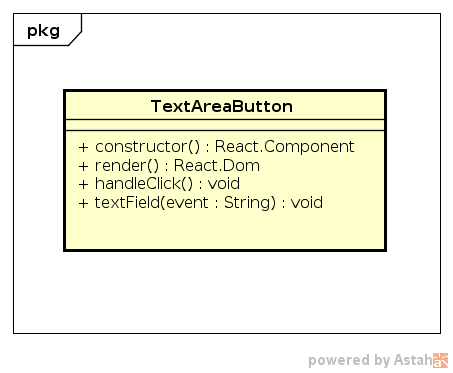
\includegraphics[width=0.6\textwidth]{img/single-TextAreaButton}
   \caption{{Diagramma per TextAreaButton in SingleComponents}}
\end{figure}
\FloatBarrier
\textbf{Descrizione}\\
Componente React che rappresenta un'area di testo con un pulsante. \\
\textbf{Metodi:} 
\begin{itemize}

\item +constructor(props : Object) : React.Component 
\\
Costruttore della sottoclasse di React.Component in cui è necessario chiamare super (props) ed è possibile inizializzare lo stato per i dati soggetti a cambiamento.

\item +textField(text : String) : void 
\\
Salva il testo scritto nella TextArea.

\item +handleClick(event : String) : void  
\\
Una volta cliccato il pulsante, passa al "padre" il testo raccolto. 

\item +render() : React.DOM 
\\
Metodo che esamina this.props e this.state e restituisce un componente React che unisce una TextArea ad un pulsate di invio.

\end{itemize} 


\textbf{Applicazioni}\\
Componente React che può essere utilizzato per la costruzione delle interfacce di alcune bolle. 


\clearpage

\subsubsection{LineEditComboBox}
\textbf{Componente:}  Monolith::UI::SingleComponents\\
   \FloatBarrier
   \begin{figure}[ht]
   \centering
   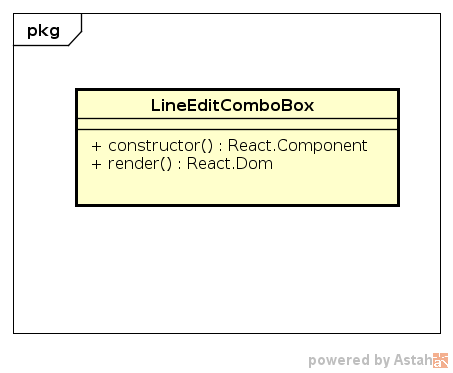
\includegraphics[width=0.6\textwidth]{img/single-LineEditComboBox}
   \caption{{Diagramma per LineEditComboBox in SingleComponents}}
\end{figure}
\FloatBarrier
\textbf{Descrizione}\\
Componente React che rappresenta una LineEdit con a fianco un ComboBox. \\
\textbf{Metodi:} 
\begin{itemize}

\item +constructor(props : Object) : React.Component 
\\
Costruttore della sottoclasse di React.Component in cui è necessario chiamare super (props) ed è possibile inizializzare lo stato per i dati soggetti a cambiamento.

\item +render() : React.DOM 
\\
Metodo che esamina this.props e this.state e restituisce un input di testo affiancato da una ComboBox.

\end{itemize} 


\textbf{Applicazioni}\\
Componente React che unisce LineEdit e ComboBox.\\
Accetta le props per la costruzione dei due componenti interni e ne ritorna i risultati al "padre" tramite le props "textUpdate" e "comboUpdate". 


\clearpage

\subsubsection{RadioButtonGroup}
\textbf{Componente:}  Monolith::UI::SingleComponents\\
   \FloatBarrier
   \begin{figure}[ht]
   \centering
   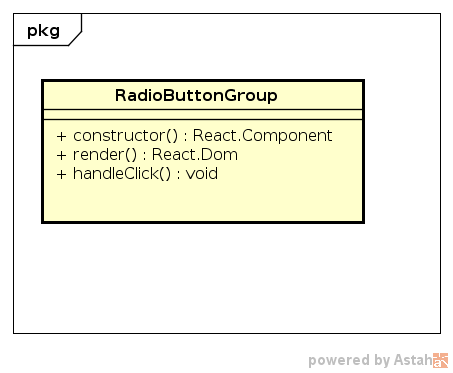
\includegraphics[width=0.6\textwidth]{img/single-RadioButtonGroup}
   \caption{{Diagramma per RadioButtonGroup in SingleComponents}}
\end{figure}
\FloatBarrier
\textbf{Descrizione}\\
Componente React che rappresenta un insieme di radio button tra cui è possibile scegliere tra opzioni mutualmente esclusive.\\

\textbf{Metodi:} 
\begin{itemize}
\item +constructor(props : Object) : React.Component 
\\
Costruttore della sottoclasse di React.Component in cui è necessario chiamare super (props) ed è possibile inizializzare lo stato per i dati soggetti a cambiamento.

\item +handleChange(event : Object): void 
\\
Viene passato al "padre" il valore selezionato.

\item +render() : React.DOM 
\\
Metodo che esamina this.props e this.state e restituisce un gruppo di RadioButton con le opzioni che sono state date.

\end{itemize} 


\textbf{Applicazioni}\\
Componente React che rappresenta un gruppo di RadioButton. \ Le opzioni vengono passate con un array attraverso la props "options". 


\clearpage

\subsubsection{TextAreaComboBox}
\textbf{Componente:}  Monolith::UI::SingleComponents\\
   \FloatBarrier
   \begin{figure}[ht]
   \centering
   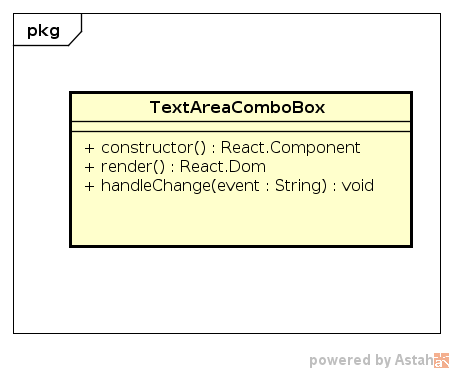
\includegraphics[width=0.6\textwidth]{img/single-TextAreaComboBox}
   \caption{{Diagramma per TextAreaComboBox in SingleComponents}}
\end{figure}
\FloatBarrier
\textbf{Descrizione}\\
Componente React che rappresenta una TextArea con a fianco un ComboBox \\
\textbf{Metodi:} 
\begin{itemize}

\item +constructor(props : Object) : React.Component 
\\
Costruttore della sottoclasse di React.Component in cui è necessario chiamare super (props) ed è possibile inizializzare lo stato per i dati soggetti a cambiamento.

\item +handleChange(event : String) : void  
\ 
Comunica al "padre" il contenuto digitato nella textarea.

\item +render() : React.DOM 
\\
Metodo che esamina this.props e this.state e restituisce un componente React composto da una textArea ed un ComboBox.

\end{itemize} 


\textbf{Applicazioni}\\
Componente React che può essere utilizzato per la costruzione delle interfacce di alcune bolle.
\ Vengono richieste anche le props per la costruzione dei degli elementi che formano il componente. 


\clearpage

\subsubsection{LineEditPushButton}
\textbf{Componente:}  Monolith::UI::SingleComponents\\
   \FloatBarrier
   \begin{figure}[ht]
   \centering
   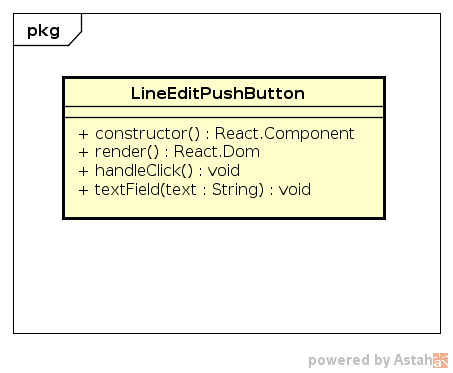
\includegraphics[width=0.6\textwidth]{img/single-LineEditPushButton}
   \caption{{Diagramma per LineEditPushButton in SingleComponents}}
\end{figure}
\FloatBarrier
\textbf{Descrizione}\\
Componente React che rappresenta un campo di inserimento testo affiancato ad un pulsante. \\
\textbf{Metodi:} 
\begin{itemize}

\item +constructor(props : Object) : React.Component 
\\
Costruttore della sottoclasse di React.Component in cui è necessario chiamare super (props) ed è possibile inizializzare lo stato per i dati soggetti a cambiamento.

\item +handleClick() : void  
\\
Passa al "padre" il testo contenuto nel LineEdit.

\item ++textField() : void  
\\
Salva nello state il testo presente nel LineEdit.

\item +render() : React.DOM 
\\
Metodo che esamina this.props e this.state e restituisce un componente React composto da un input di testo ed un pulsante di invio.

\end{itemize} 


\textbf{Applicazioni}\\
Viene utilizzato per costruire alcune interfacce grafiche delle bolle.
Oltre alle props dei due componenti React, il componente si aspetta le seguenti props:
\begin{itemize}

\item classesle:
\\
Stile CSS per il LineEdit.
\item classespb:
\ 
Stile CSS per il PushButton.

\item idle:
\\
ID per il LineEdit.
\item idpb: 
\\
ID per il PushButton.
\end{itemize} 


\clearpage

\subsubsection{AbsBubble}
\textbf{Componente:}  Monolith::UI::uiConstruction\\
   \FloatBarrier
   \begin{figure}[ht]
   \centering
   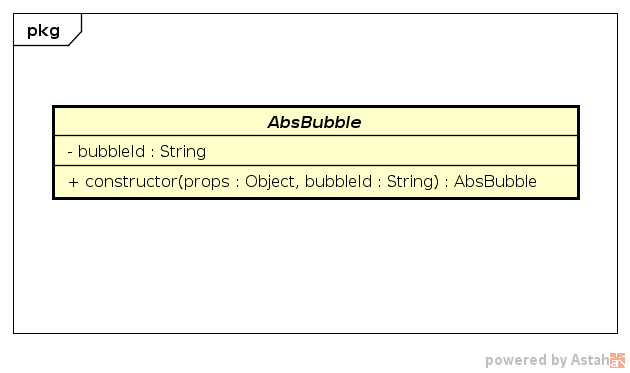
\includegraphics[width=0.6\textwidth]{img/single-AbsBubble}
   \caption{{Diagramma per AbsBubble in uiConstruction}}
\end{figure}
\FloatBarrier
\textbf{Descrizione}\\
Classe base astratta per le interfacce grafiche delle singole bolle. 


\textbf{Applicazioni}\\
Viene utilizzata come classe base da cui derivare le interfacce grafiche delle bolle. 


\clearpage

\subsubsection{AbsButton}
\textbf{Componente:}  Monolith::UI::uiConstruction\\
   \FloatBarrier
   \begin{figure}[ht]
   \centering
   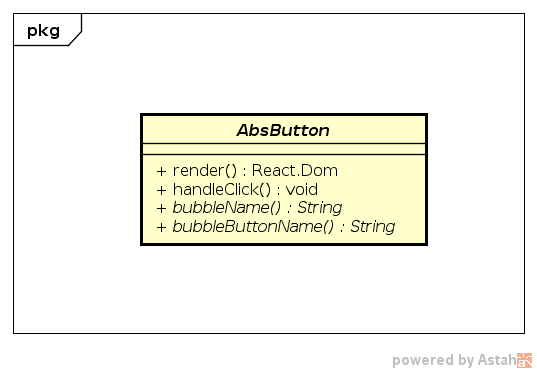
\includegraphics[width=0.6\textwidth]{img/single-AbsButton}
   \caption{{Diagramma per AbsButton in uiConstruction}}
\end{figure}
\FloatBarrier
\textbf{Descrizione}\\
Classe base dei pulsanti del menu di creazione delle nuove bolle. La classe base contiene molto codice e chiede classi derivate relativamente semplici. Viene usato il template pattern per parametrizzare gli aspetti che differiscono tra le classi derivate.
I seguenti metodi sono astratti puri:
\begin{itemize}
\item +bubbleName(): String \\
Nelle classi derivate ritorna il nome della bolla necessario per usare BubbleDiscriminator
\item +bubbleButtonName(): String \\
Nelle classi derivate ritorna il testo che deve comparire nel pulsante
\item +secondAreaName(): String \\
Nelle classi derivate ritorna il nome del componente React che deve essere inserito alla pressione del secondo pulsante. \'E necessario per usare BubbleDiscriminator
\end{itemize}
I seguenti metodi semplicemente eseguono le funzioni che vengono passate nelle props in risposta alla pressione dei pulsanti:
\begin{itemize}
\item +handleClick():void
\item +handleSecondButton():void
\end{itemize}
Il metodo render crea uno o due pulsanti a seconda che sia definito o meno il testo da inserire nel secondo pulsante nelle props. 


\textbf{Applicazioni}\\
Classe base da cui derivare per ottenere i pulsanti del menu di creazione di di nuove bolle 


\clearpage

\subsubsection{bubbleCreator}
\textbf{Componente:}  Monolith::UI::uiConstruction\\
   \FloatBarrier
   \begin{figure}[ht]
   \centering
   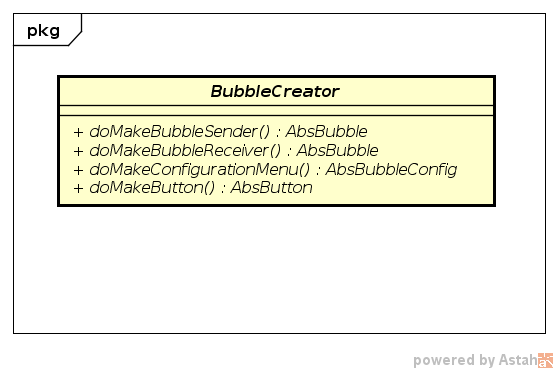
\includegraphics[width=0.6\textwidth]{img/single-bubbleCreator}
   \caption{{Diagramma per bubbleCreator in uiConstruction}}
\end{figure}
\FloatBarrier
\textbf{Descrizione}\\
Classe base astratta da cui poter derivare le classi concrete che si occupano della creazione delle istanze  di componenti grafici  \ 
\textbf{Metodi:}
\begin{itemize}
\item +doMakeBubbleSender() : ConcreteBubble 
\\
Ritorna il componente React per visualizzare una bolla inviata.
\item +doMakeBubbleReceiver() : ConcreteBubble 
\ 
Ritorna il componente React per visualizzare una bolla ricevuta.
\item +doMakeConfigurationMenu() : ConcreteBubbleConfig 
\\
Ritorna il componente React per visualizzare il menù di creazione di una bolla da inviare.
\item +doMakeButton() : ConcreteBubbleCreationButton 
\ 
Ritorna il componente React per visualizzare il bottone di creazione del menù di configurazione di una bolla da inviare.

\end{itemize} 


\textbf{Applicazioni}\\
Interfaccia che viene utilizzata come rappresentazione di concreteBubbleCreator. 


\clearpage

\subsubsection{AbsBubbleConfig}
\textbf{Componente:}  Monolith::UI::uiConstruction\\
   \FloatBarrier
   \begin{figure}[ht]
   \centering
   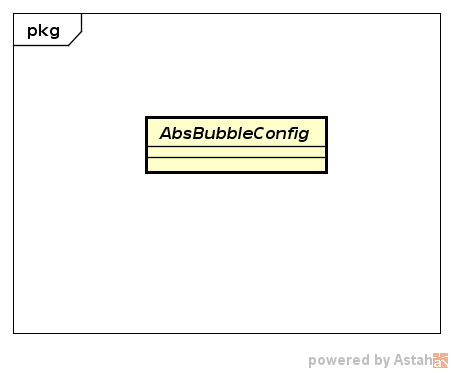
\includegraphics[width=0.6\textwidth]{img/single-AbsBubbleConfig}
   \caption{{Diagramma per AbsBubbleConfig in uiConstruction}}
\end{figure}
\FloatBarrier
\textbf{Descrizione}\\
Classe Astratta (interfaccia) per i menù di configurazione delle singole bolle. 


\textbf{Applicazioni}\\
Classe base da cui derivare per costruire i menù di configurazione delle bolle. 


\clearpage

\subsubsection{bubbleDiscriminator}
\textbf{Componente:}  Monolith::UI::uiConstruction\\
   \FloatBarrier
   \begin{figure}[ht]
   \centering
   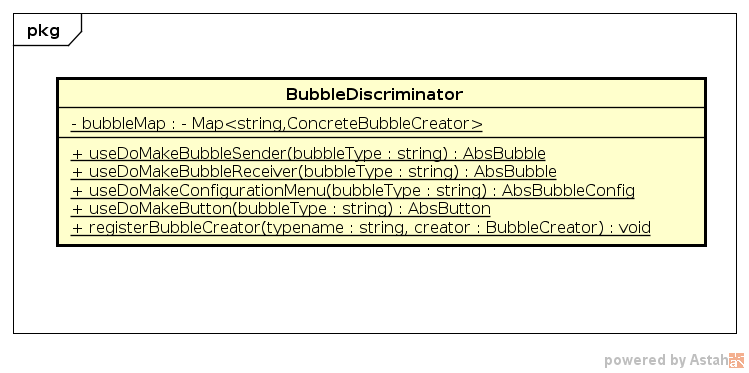
\includegraphics[width=0.6\textwidth]{img/single-bubbleDiscriminator}
   \caption{{Diagramma per bubbleDiscriminator in uiConstruction}}
\end{figure}
\FloatBarrier
\textbf{Descrizione}\\
Classe che contiene i metodi che ritornano le funzionalità necessarie per la rappresentazione delle bolle.

\textbf{Attributi:}
\begin{itemize}
\item -bubbleMap : Map$<$string,concreteBubbleCreator$>$ 
\\
Struttura che mappa il nome di una bolla con l'istanza di concreteBubbleCreator per quella bolla.
\end{itemize}
\textbf{Metodi:} 
\begin{itemize}
\item +useDoMakeBubbleSender( bubbleType: string) : ConcreteBubble \\
Ritorna il componente React della stringa passata come parametro per visualizzare una bolla inviata.
\item +useDoMakeBubbleReceiver( bubbleType: string) : ConcreteBubble \\
Ritorna il componente React della stringa passata come parametro per visualizzare una bolla ricevuta.
\item +useDoMakeBubbleConfigurationMenu( bubbleType: string) : ConcreteBubbleConfig 
\\
Ritorna il componente React della stringa passata come parametro per visualizzare il menù di creazione di una bolla da inviare.
\item  +useDoMakeButton( bubbleType: string) : ConcreteBubbleCreationButton \\
Ritorna il componente React della stringa passata come parametro per visualizzare il bottone di creazione del menù di configurazione di una bolla da inviare.

\end{itemize} 


\textbf{Applicazioni}\\
Viene utilizzata quando si deve creare una nuova bolla, ritornando l'oggetto della bolla appena selezionata. 


\subsection{Architettura di dettaglio - Classi delle bolle demo}\subsubsection{CurrencyBubble}
\textbf{Componente:}  CurrencyBubble\\
   \FloatBarrier
   \begin{figure}[ht]
   \centering
   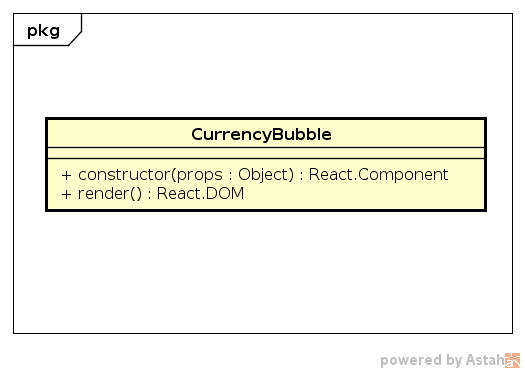
\includegraphics[width=0.6\textwidth]{img/single-CurrencyBubble}
   \caption{{Diagramma per CurrencyBubble in CurrencyBubble}}
\end{figure}
\FloatBarrier
\textbf{Descrizione}\\
Componente React che rappresenta l'interfaccia grafica di una CurrencyBubble
\\
\textbf{Metodi:} 
\begin{itemize}
\item +constructor(props : Object) : React.Component 
\\
Costruttore della sottoclasse di React.Component in cui è necessario chiamare super (props) ed è possibile inizializzare lo stato per i dati soggetti a cambiamento.

\item +render() : React.DOM 
\\
Metodo che esamina this.props e this.state e restituisce la CurrencyBubble a conversione avvenuta.

\end{itemize} 


\textbf{Applicazioni}\\
Viene utilizzata per rappresentare graficamente la bolla di conversione valuta.
Il componente CurrencyBubble si aspetta in entrata le props contenetenti i dati di conversione: \\
\begin{itemize}
\item \textit{curr\_in}:
\\
Valore della valuta base.

\item \textit{curr\_out}:
\\
Valore della valuta d'uscita.

\item \textit{value\_in}:
\\
Valore di conversione iniziale.

\item \textit{value\_out}:
\\
Valore finale di conversione.
\end{itemize} 


\clearpage

\subsubsection{CurrencyCreator}
\textbf{Componente:}  CurrencyBubble\\
   \FloatBarrier
   \begin{figure}[ht]
   \centering
   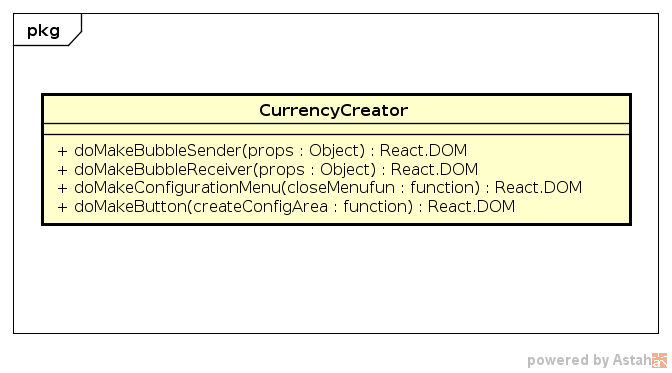
\includegraphics[width=0.6\textwidth]{img/single-CurrencyCreator}
   \caption{{Diagramma per CurrencyCreator in CurrencyBubble}}
\end{figure}
\FloatBarrier
\textbf{Descrizione}\\
Istanziazione concreta della classe Monolith::UI::Bubbles::BubbleCreator che gestisce la creazione della singola istanza di bolla convertitore di valuta, della singola istanza di menù di configurazione della bolla e della singola istanza di pulsante tramite l'utilizzo della classe Monolith::UI::Bubbles::BubbleDiscriminator.
\\
\textbf{Metodi:} 
\begin{itemize}
\item +doMakeBubbleSender() : CurrencyBubble 
\\
Metodo che gestisce la creazione della bolla vista dal mittente.
\item +doMakeBubbleReceiver() : CurrencyBubble 
\\
Metodo che gestisce la creazione della bolla vista dal ricevente.
\item +doMakeConfigurationMenu() : CurrencyBubbleConfig 
\\
Metodo che gestisce la creazione dell'area di configurazione della bolla.
\item +doMakeButton() : CurrencyBubbleCreationButton 
\\
Metodo che gestisce la creazione della singola istanza di pulsante da inserire nel menu iniziale di creazione. Viene lasciata l'implementazione della super classe.
\end{itemize} 


\textbf{Applicazioni}\\
Viene utilizzata per gestire la creazione della singola istanza di bolla convertitore di valuta, della singola istanza di menù di configurazione della bolla e della singola istanza di pulsante. 


\clearpage

\subsubsection{CurrencyBubbleConfig}
\textbf{Componente:}  CurrencyBubble\\
   \FloatBarrier
   \begin{figure}[ht]
   \centering
   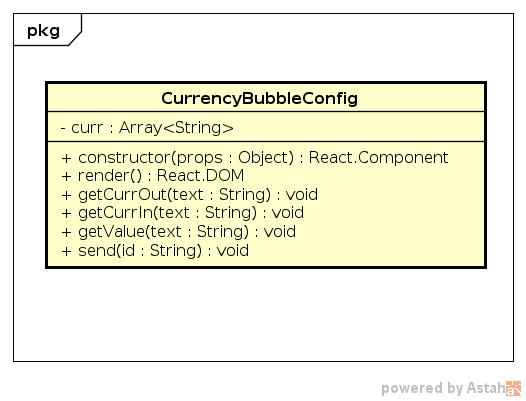
\includegraphics[width=0.6\textwidth]{img/single-CurrencyBubbleConfig}
   \caption{{Diagramma per CurrencyBubbleConfig in CurrencyBubble}}
\end{figure}
\FloatBarrier
\textbf{Descrizione}\\
Componente React che rappresenta il menù per la costruzione di una bolla di conversione valuta.
\\
\textbf{Metodi:} 
\begin{itemize}
\item +constructor(props : Object) : React.Component 
\\
Costruttore della sottoclasse di React.Component in cui è necessario chiamare super (props) ed è possibile inizializzare lo stato per i dati di conversione e per quelli soggetti a cambiamento.

\item +getCurrIn(text : String) : void 
\\
Salva la valuta di base.

\item +getCurrOut(text : String) : void 
\\
Salva la valuta di uscita.

\item +getValue(text : String) : void 
\\
Salva il valore iniziale di conversione.

\item +send() : void 
\\
Salva i dati raccolti e li passa al "padre".

\item +render() : React.DOM
\\
Metodo che esamina this.props e this.state, costruisce un array di opzioni modificabili e restituisce l'interfaccia grafica per il menù di creazione.
\end{itemize} 


\textbf{Applicazioni}\\
Viene utilizzato per rappresentare il menù di configurazione della bolla di conversione valuta. Il componente React si aspetta, nella props "send", una funzioni che raccolga un oggetto contenente i dati della bolla. 


\clearpage

\subsubsection{CurrencyBubbleCreationButton}
\textbf{Componente:}  CurrencyBubble\\
   \FloatBarrier
   \begin{figure}[ht]
   \centering
   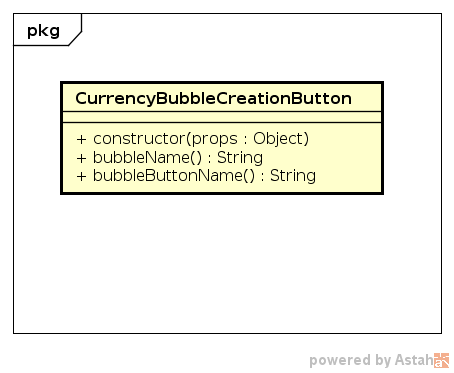
\includegraphics[width=0.6\textwidth]{img/single-CurrencyBubbleCreationButton}
   \caption{{Diagramma per CurrencyBubbleCreationButton in CurrencyBubble}}
\end{figure}
\FloatBarrier
\textbf{Descrizione}\\
Componente React che rappresenta il pulsante per creare una bolla di conversione valuta.
\\
\textbf{Metodi:} 
\begin{itemize}
\item +constructor(props : Object) : React.Component 
\\
Costruttore della sottoclasse di React.Component in cui è necessario chiamare super (props) ed è possibile inizializzare lo stato per i dati soggetti a cambiamento.

\item +bubbleButtonName() : String 
\\
Metodo che ritorna il nome presente sul pulsante.

\item +bubbleName() : String 
\\
Metodo che ritorna il nome identificativo della bolla .

\end{itemize} 


\textbf{Applicazioni}\\
Viene utilizzato per rappresentare il pulsante per la creazione di una bolla di conversione valuta.

Nella props "onClick" verrà ritornato il nome identificativo della bolla. 


\clearpage

\subsubsection{ListBubbleConfig}
\textbf{Componente:}  ListBubble::CheckListCreation\\
   \FloatBarrier
   \begin{figure}[ht]
   \centering
   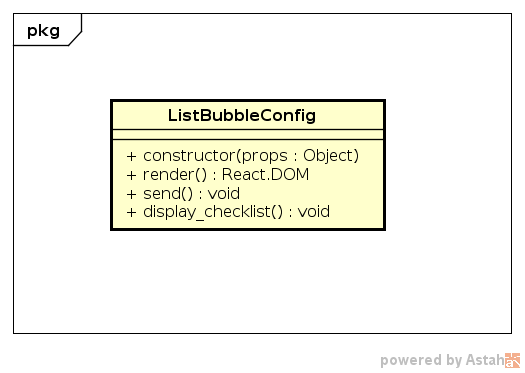
\includegraphics[width=0.6\textwidth]{img/single-ListBubbleConfig}
   \caption{{Diagramma per ListBubbleConfig in CheckListCreation}}
\end{figure}
\FloatBarrier
\textbf{Descrizione}\\
Componente React che rappresenta il menù per la costruzione di una bolla Lista.
\\
\textbf{Metodi:} 
\begin{itemize}
\item +constructor(props : Object) : React.Component 
\\
Costruttore della sottoclasse di React.Component in cui è necessario chiamare super (props) ed è possibile inizializzare lo stato per i dati soggetti a cambiamento.

\item +addOpt() : void 
\\
Aggiunge un campo opzione in più ad ogni click sul tasto apposito.

\item +titleChange() : void 
\\
Salva il titolo che viene dato alla Lista.

\item +optChange() : void 
\\
Salva il valore che viene dato ad ogni opzione.

\item +send() : void 
\\
Salva i dati raccolti e li passa al "padre".

\item +render() : React.DOM
\\
Metodo che esamina this.props e this.state, costruisce un array di opzioni modificabili e restituisce l'interfaccia grafica per il menù di creazione.
\end{itemize} 


\textbf{Applicazioni}\\
Viene utilizzato per rappresentare il menù di configurazione della bolla Lista. Il componente React si aspetta, nella props "send", una funzione che raccolga un oggetto contenente i dati della bolla. 


\clearpage

\subsubsection{ListBubbleCreationButton}
\textbf{Componente:}  ListBubble::CheckListCreation\\
   \FloatBarrier
   \begin{figure}[ht]
   \centering
   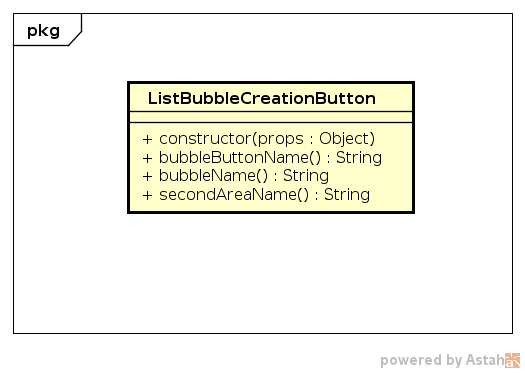
\includegraphics[width=0.6\textwidth]{img/single-ListBubbleCreationButton}
   \caption{{Diagramma per ListBubbleCreationButton in CheckListCreation}}
\end{figure}
\FloatBarrier
\textbf{Descrizione}\\
Componente React che rappresenta il pulsante per creare una bolla Lista.
\\
\textbf{Metodi:} 
\begin{itemize}
\item +constructor(props : Object) : React.Component 
\\
Costruttore della sottoclasse di React.Component in cui è necessario chiamare super (props) ed è possibile inizializzare lo stato per i dati soggetti a cambiamento.

\item +bubbleButtonName() : String 
\\
Metodo che ritorna il nome presente sul pulsante.

\item +bubbleName() : String 
\\
Metodo che ritorna il nome identificativo della bolla .

\end{itemize} 


\textbf{Applicazioni}\\
Viene utilizzato per rappresentare il pulsante per la creazione di una bolla Lista.

Nella props "onClick" verrà ritornato il nome identificativo della bolla. 


\clearpage

\subsubsection{ListBubble}
\textbf{Componente:}  ListBubble::CheckListReading\\
   \FloatBarrier
   \begin{figure}[ht]
   \centering
   \includegraphics[width=0.6\textwidth]{img/single-ListBubble}
   \caption{{Diagramma per ListBubble in CheckListReading}}
\end{figure}
\FloatBarrier
\textbf{Descrizione}\\
Componente React che rappresenta l'interfaccia grafica di una ListBubble
\\
\textbf{Metodi:} 
\begin{itemize}
\item +constructor(props : Object) : React.Component 
\\
Costruttore della sottoclasse di React.Component in cui è necessario chiamare super (props) ed è possibile inizializzare lo stato per i dati soggetti a cambiamento.

\item +render() : React.DOM 
\\
Metodo che esamina this.props e this.state e restituisce elemento CheckBoxList 

\item +changeCheck(m : Object) : void \\
Metodo che passa al "padre" i dati relativi alla checkbox cliccata.
\end{itemize} 


\textbf{Applicazioni}\\
Viene utilizzata per rappresentare graficamente la bolla Lista.
Il componente ListBubble si aspetta in entrata una props "stat" che dovrà contenere un oggetto con i seguenti dati: \\
\begin{itemize}
\item \textit{op}:
\\
Un array di opzioni aventi un campo "id" ed un campo "value".
\item \textit{title}:
\\
Un titolo per la Lista.
\end{itemize} 


\clearpage

\subsubsection{ListDb}
\textbf{Componente:}  ListBubble::Configuration\\
   \FloatBarrier
   \begin{figure}[ht]
   \centering
   \includegraphics[width=0.6\textwidth]{img/single-ListDb}
   \caption{{Diagramma per ListDb in Configuration}}
\end{figure}
\FloatBarrier
\textbf{Descrizione}\\
 


\textbf{Applicazioni}\\
 


\clearpage

\subsubsection{ListCheck}
\textbf{Componente:}  ListBubble::DataManagement\\
   \FloatBarrier
   \begin{figure}[ht]
   \centering
   \includegraphics[width=0.6\textwidth]{img/single-ListCheck}
   \caption{{Diagramma per ListCheck in DataManagement}}
\end{figure}
\FloatBarrier
\textbf{Descrizione}\\
 


\textbf{Applicazioni}\\
 


\clearpage

\subsubsection{ListBubbleCreator}
\textbf{Componente:}  ListBubble::DataManagement\\
   \FloatBarrier
   \begin{figure}[ht]
   \centering
   \includegraphics[width=0.6\textwidth]{img/single-ListBubbleCreator}
   \caption{{Diagramma per ListBubbleCreator in DataManagement}}
\end{figure}
\FloatBarrier
\textbf{Descrizione}\\
Istanziazione concreta della classe Monolith::UI::Bubbles::BubbleCreator che gestisce la creazione della singola istanza di bolla lista, della singola istanza di menù di configurazione della bolla e della singola istanza di pulsante tramite l'utilizzo della classe Monolith::UI::Bubbles::BubbleDiscriminator.
\\
\textbf{Metodi:} 
\begin{itemize}
\item +doMakeBubbleSender() : ListBubble 
\\
Metodo che gestisce la creazione della bolla vista dal mittente.
\item +doMakeBubbleReceiver() : ListBubble 
\\
Metodo che gestisce la creazione della bolla vista dal ricevente.
\item +doMakeConfigurationMenu() : ListBubbleConfig 
\\
Metodo che gestisce la creazione dell'area di configurazione della bolla.
\item +doMakeButton() : ListBubbleCreationButton 
\\
Metodo che gestisce la creazione dello specifico pulsante da inserire nel menu iniziale di creazione.
\end{itemize} 


\textbf{Applicazioni}\\
Viene utilizzata per gestire la creazione della singola istanza di bolla lista, della singola istanza di menù di configurazione della bolla e della singola istanza di pulsante. 


\clearpage

\subsubsection{PollBubble}
\textbf{Componente:}  PollBubble\\
   \FloatBarrier
   \begin{figure}[ht]
   \centering
   \includegraphics[width=0.6\textwidth]{img/single-SurveyBubble}
   \caption{{Diagramma per PollBubble in PollBubble}}
\end{figure}
\FloatBarrier
\textbf{Descrizione}\\
Componente React che rappresenta l'interfaccia grafica di una PollBubble
\\
\textbf{Metodi:} 
\begin{itemize}
\item +constructor(props : Object) : React.Component 
\\
Costruttore della sottoclasse di React.Component in cui è necessario chiamare super (props) ed è possibile inizializzare lo stato per i dati soggetti a cambiamento.

\item +render() : React.DOM 
\\
Metodo che esamina this.props e this.state e restituisce una lista di PushButton per votare il sondaggio. 

\item +addVoto(id : String) : void \\
Metodo che da un voto all'opzione selezionata. Permette di votare una sola volta.

\end{itemize} 


\textbf{Applicazioni}\\
Viene utilizzata per rappresentare graficamente la bolla Sondaggio.
Il componente PollBubble si aspetta in entrata i seguenti dati: \\
\begin{itemize}
\item \textit{op}:
\\
Un array di opzioni.
\item \textit{title}:
\\
Un titolo per il sondaggio.
\item \textit{num}:
\\
Il numero delle opzioni.
\item \textit{id}:
\\
Un ID per la bolla Sondaggio.
\end{itemize} 


\clearpage

\subsubsection{PollCreator}
\textbf{Componente:}  PollBubble\\
   \FloatBarrier
   \begin{figure}[ht]
   \centering
   \includegraphics[width=0.6\textwidth]{img/single-SurveyCreator}
   \caption{{Diagramma per PollCreator in PollBubble}}
\end{figure}
\FloatBarrier
\textbf{Descrizione}\\
Istanziazione concreta della classe Monolith::UI::Bubbles::BubbleCreator che gestisce la creazione della singola istanza di bolla sondaggio, della singola istanza di menù di configurazione della bolla e della singola istanza di pulsante tramite l'utilizzo della classe Monolith::UI::Bubbles::BubbleDiscriminator.
\\
\textbf{Metodi:} 
\begin{itemize}
\item +doMakeBubbleSender() : SurveyBubble 
\\
Metodo che gestisce la creazione della bolla vista dal mittente.
\item +doMakeBubbleReceiver() : SurveyBubble 
\\
Metodo che gestisce la creazione della bolla vista dal ricevente.
\item +doMakeConfigurationMenu() : SurveyBubbleConfig 
\\
Metodo che gestisce la creazione dell'area di configurazione della bolla.
\item +doMakeButton() : SurveyBubbleCreationButton 
\\
Metodo che gestisce la creazione della singola istanza di pulsante da inserire nel menu iniziale di creazione. Viene lasciata l'implementazione della super classe.
\end{itemize} 


\textbf{Applicazioni}\\
Viene utilizzata per gestire la creazione della singola istanza di bolla sondaggio, della singola istanza di menù di configurazione della bolla e della singola istanza di pulsante. 


\clearpage

\subsubsection{PollBubbleConfig}
\textbf{Componente:}  PollBubble\\
   \FloatBarrier
   \begin{figure}[ht]
   \centering
   \includegraphics[width=0.6\textwidth]{img/single-SurveyBubbleConfigMenu}
   \caption{{Diagramma per PollBubbleConfig in PollBubble}}
\end{figure}
\FloatBarrier
\textbf{Descrizione}\\
Componente React che rappresenta il menù per la costruzione di una bolla Sondaggio.
\\
\textbf{Metodi:} 
\begin{itemize}
\item +constructor(props : Object) : React.Component 
\\
Costruttore della sottoclasse di React.Component in cui è necessario chiamare super (props) ed è possibile inizializzare lo stato per i dati soggetti a cambiamento.

\item +addOpt() : void 
\\
Aggiunge un campo opzione in più ad ogni click sul tasto apposito.

\item +titleChange() : void 
\\
Salva il titolo che viene dato alla Lista.

\item +optChange() : void 
\\
Salva i valori che vengono dati ad ogni opzione.

\item +send() : void 
\\
Salva i dati raccolti e li passa al "padre".

\item +render() : React.DOM \\
Metodo che esamina this.props e this.state, costruisce un array di opzioni modificabili e restituisce l'interfaccia grafica per il menù di creazione.
\end{itemize} 


\textbf{Applicazioni}\\
Viene utilizzato per rappresentare il menù di configurazione della bolla Sondaggio. Il componente React si aspetta, nella props "send", una funzione che raccolga un oggetto contenente i dati della bolla. 


\clearpage

\subsubsection{PollBubbleCreationButton}
\textbf{Componente:}  PollBubble\\
   \FloatBarrier
   \begin{figure}[ht]
   \centering
   \includegraphics[width=0.6\textwidth]{img/single-SurveyBubbleCreationButton}
   \caption{{Diagramma per PollBubbleCreationButton in PollBubble}}
\end{figure}
\FloatBarrier
\textbf{Descrizione}\\
Componente React che rappresenta il pulsante per creare una bolla Sondaggio.
\\
\textbf{Metodi:} 
\begin{itemize}
\item +constructor(props : Object) : React.Component 
\\
Costruttore della sottoclasse di React.Component in cui è necessario chiamare super (props) ed è possibile inizializzare lo stato per i dati soggetti a cambiamento.

\item +bubbleButtonName() : String 
\\
Metodo che ritorna il nome presente sul pulsante.

\item +bubbleName() : String 
\\
Metodo che ritorna il nome identificativo della bolla .

\end{itemize} 


\textbf{Applicazioni}\\
Viene utilizzato per rappresentare il pulsante per la creazione di una bolla Sondaggio.

Nella props "onClick" verrà ritornato il nome identificativo della bolla. 


\clearpage

\subsubsection{RandBubble}
\textbf{Componente:}  RandomBubble\\
   \FloatBarrier
   \begin{figure}[ht]
   \centering
   \includegraphics[width=0.6\textwidth]{img/single-DiceBubble}
   \caption{{Diagramma per RandBubble in RandomBubble}}
\end{figure}
\FloatBarrier
\textbf{Descrizione}\\
Componente React che rappresenta l'interfaccia grafica di una RandBubble
\\
\textbf{Metodi:} 
\begin{itemize}
\item +constructor(props : Object) : React.Component 
\\
Costruttore della sottoclasse di React.Component in cui è necessario chiamare super (props) ed è possibile inizializzare lo stato per i dati soggetti a cambiamento. 

\item +render() : React.DOM 
\\
Metodo che esamina this.props e this.state e restituisce il numero random calcolato. 

\item +calcolate() : void \\
Metodo che passa al "padre" il nuovo numero random estratto.
\end{itemize} 


\textbf{Applicazioni}\\
Viene utilizzata per rappresentare graficamente la bolla Random.
Il componente RandBubble si aspetta in entrata una props "nMax" che dovrà contenere il numero delle facce del dado. 


\clearpage

\subsubsection{RandCreator}
\textbf{Componente:}  RandomBubble\\
   \FloatBarrier
   \begin{figure}[ht]
   \centering
   \includegraphics[width=0.6\textwidth]{img/single-DiceBubbleCreator}
   \caption{{Diagramma per RandCreator in RandomBubble}}
\end{figure}
\FloatBarrier
\textbf{Descrizione}\\
Istanziazione concreta della classe Monolith::UI::Bubbles::BubbleCreator che gestisce la creazione della singola istanza di bolla estrazione di numero casuale, della singola istanza di menù di configurazione della bolla e della singola istanza di pulsante tramite l'utilizzo della classe Monolith::UI::Bubbles::BubbleDiscriminator.
\\
\textbf{Metodi:} 
\begin{itemize}
\item +doMakeBubbleSender() : DiceBubble 
\\
Metodo che gestisce la creazione della bolla vista dal mittente.
\item +doMakeBubbleReceiver() : DiceBubble 
\\
Metodo che gestisce la creazione della bolla vista dal ricevente.
\item +doMakeConfigurationMenu() : DiceBubbleConfig 
\\
Metodo che gestisce la creazione dell'area di configurazione della bolla.
\item +doMakeButton() : DiceBubbleCreationButton 
\\
Metodo che gestisce la creazione della singola istanza di pulsante da inserire nel menu iniziale di creazione. Viene lasciata l'implementazione della super classe.
\end{itemize} 


\textbf{Applicazioni}\\
Viene utilizzata per gestire la creazione della singola istanza di bolla estrazione di numero casuale, della singola istanza di menù di configurazione della bolla e della singola istanza di pulsante. 


\clearpage

\subsubsection{RandBubbleConfig}
\textbf{Componente:}  RandomBubble\\
   \FloatBarrier
   \begin{figure}[ht]
   \centering
   \includegraphics[width=0.6\textwidth]{img/single-DiceBubbleConfigMenu}
   \caption{{Diagramma per RandBubbleConfig in RandomBubble}}
\end{figure}
\FloatBarrier
\textbf{Descrizione}\\
Componente React che rappresenta il menù per la costruzione di una bolla di conversione valuta.
\\
\textbf{Metodi:} 
\begin{itemize}
\item +constructor(props : Object) : React.Component 
\\
Costruttore della sottoclasse di React.Component in cui è necessario chiamare super (props) ed è possibile inizializzare lo stato per i dati soggetti a cambiamento.

\item +getValue(val: String) : void 
\\
Salva il numero di facce del dado.

\item +send() : void 
\\
Salva i dati raccolti e li passa al "padre".

\item +render() : React.DOM \\
Metodo che esamina this.props e this.state e restituisce l'interfaccia grafica per il menù di creazione.
\end{itemize} 


\textbf{Applicazioni}\\
Viene utilizzato per rappresentare il menù di configurazione della bolla di lancio casuale di dadi. Il componente React si aspetta, nella props "send", una funzioni che raccolga un oggetto contenente i dati della bolla. 


\clearpage

\subsubsection{RandBubbleCreationButton}
\textbf{Componente:}  RandomBubble\\
   \FloatBarrier
   \begin{figure}[ht]
   \centering
   \includegraphics[width=0.6\textwidth]{img/single-diceBubbleCreationButton}
   \caption{{Diagramma per RandBubbleCreationButton in RandomBubble}}
\end{figure}
\FloatBarrier
\textbf{Descrizione}\\
Componente React che rappresenta il pulsante per creare una bolla di lancio casuale di dadi.
\\
\textbf{Metodi:} 
\begin{itemize}
\item +constructor(props : Object) : React.Component 
\\
Costruttore della sottoclasse di React.Component in cui è necessario chiamare super (props) ed è possibile inizializzare lo stato per i dati soggetti a cambiamento.

\item +bubbleButtonName() : String 
\\
Metodo che ritorna il nome presente sul pulsante.

\item +bubbleName() : String 
\\
Metodo che ritorna il nome identificativo della bolla .

\end{itemize} 


\textbf{Applicazioni}\\
Viene utilizzato per rappresentare il pulsante per la creazione di una bolla di lancio casuale di dadi.

Nella props "onClick" verrà ritornato il nome identificativo della bolla. 




\subsection{Architettura di dettaglio - Schema dei dati per il
  database}
\subsubsection{Sintassi SimpleSchema}

Segue un semplicissimo esempio di come si può rappresentare lo schema
su cui gli oggetti devono essere validati. Lo schema è descritto con
un oggetto.

\begin{lstlisting}
{
  firstName: {
    type: String
  },
  age: {
    type: Number
  },
  comments: {
    type: [String]
  }
}
\end{lstlisting}

Questo esempio descrive 3 campi dati. Ciascun campo deve essere
presente nell'oggetto da validare ma l'ordine non è rilevante.
\begin{itemize}
\item \textbf{firstName} campo dati di tipo stringa
\item \textbf{age} campo dati di tipo numerico
\item \textbf{comments} campo dati di tipo array di stringhe
\end{itemize}
Per una documentazione estesa di veda il link alla documentazione del
pacchetto presente in \S 1.4.2

\subsubsection{Bolla Currency}
\begin{lstlisting}
{
	curr_in:{
		label: 'Currency of input',
		type: String
	},
	curr_out:{
		label: 'Currency of output',
		type: String
	},
	value_in:{
		type: Number,
		label: 'Value to be converted'
	},
	value_out:{
		type: Number,
		label: 'Value converted'
}
\end{lstlisting}

\subsubsection{Bolla Lista}
\begin{lstlisting}
\end{lstlisting}

\subsubsection{Bolla Poll}
\begin{lstlisting}
\end{lstlisting}

\subsubsection{Bolla Random}
\begin{lstlisting}
\end{lstlisting}

\subsection{Giustificazione dell'utilizzo di oggetti globali}

%%%%%%%%%%%%%%%%%%%%%%%%%%%%%%%%%%%%%%%%%%%%%%%%%%%%%%%%%%%%%%%%%%%%%%%%%%%%%%%
\section{Standard di Progetto}
%\subsection{Standard di progettazione architetturale}

\subsection{Standard di documentazione del codice}
Gli standard di documentazione del codice sono definiti nel
documento  \emph{\normediprogetto} .

\subsection{Standard di denominazione di entità e relazioni }
Gli standard di denominazione sono definiti nel nel
documento  \emph{\normediprogetto} .

%\subsection{Standard di programmazione}
%Gli standard di programmazione sono definiti nel nel
%documento NormeDiProgetto
\subsection{Strumenti di lavoro}
Gli strumenti da utilizzare e le procedure da seguire sono descritti
nel documento  \emph{\normediprogetto} .


\section{Diagrammi di Attività}
Il diagramma delle attività è un diagramma definito all'interno dello
Unified Modeling Language (UML) che definisce le attività da svolgere
per realizzare una data funzionalità. Può essere utilizzato durante la
progettazione del software per dettagliare un determinato
algoritmo. Più in dettaglio, un activity diagram definisce una serie
di attività o flusso, anche in termini di relazioni tra le attività, i
responsabili per le singole attività e i punti di
decisione. L'activity diagram è spesso usato come modello
complementare allo Use Case Diagram, per descrivere le dinamiche con
cui si sviluppano i diversi use case. 

\subsection{Configurazione sondaggio}
Questo diagramma rappresenta la configurazione e l'invio della bolla
sondaggio. L’utente inserisce il titolo del sondaggio, dopodichè
avviene l’inserimento delle opzioni. L’utente ha la possibilità di
inserire più opzioni (rappresentato nel diagramma con la freccia che
parte dal nodo decisione e raggiunge il nodo azione chiamato inserisci
opzioni). Una volta compiuto il processo di configurazione l’utente
decide di inviare la bolla (rappresentato dal nodo invia). Se il
numero delle opzioni inserite è minore di due allora il flusso ritorna
al nodo azione chiamato “inserisci opzione” per poter permettere
all’utente di incrementare il numero delle opzioni del
sondaggio. Altrimenti (il numero di opzioni è maggiore di uno) il
flusso arriva al nodo di fine dell’attività. 

\begin{center}
  \includegraphics[scale=0.5]{img/Sondaggio.jpg}
  \captionof{figure}{Diagramma di attività per la bolla sondaggio} 
\end{center}


\subsection{Configurazione ListBubble}
Questo diagramma rappresenta la configurazione della bolla
ListBubble. Il flusso inizia con l’inserimento del titolo della
lista. Dopo questo processo il flusso raggiunge il nodo decisione dove
l’utente sceglie il modo di inserimento degli elementi. L’inserimento
degli elementi avviene o manualmente (inserisci elemento manualmente)
oppure con la selezione nella lista degli elementi predefiniti
(inserisci elemento da checklist). Nel caso l’utente scegliesse di
inserire un elemento dalla checklist predefinita, il flusso raggiunge
il nodo decisione. Da questo punto l’utente può scegliere di inviare
la bolla già configurata e il flusso raggiunge il nodo terminale,
oppure scegliere di ritornare nel nodo decisione raggiunto
precedentemente per poter inserire un altro elemento. Anche nel caso
in cui l’utente scegliesse di inserire un elemento manualmente il
flusso segue lo stesso percorso, ovvero l’utente inserisce l’elemento
e decide di inviare la bolla con il raggiungere il nodo terminale
oppure inserire un altro elemento. 

\begin{center}
  \includegraphics[scale=0.5]{img/ListBubble.png}
  \captionof{figure}{Diagramma di attività per la bolla ListBubble}
\end{center}



\section{Diagramma di Sequenza}

\subsection{Creazione Bolla}


	\includegraphics[width=\textwidth]{img/CreationBubble.png}
	\captionof{figure}{Diagramma di sequenza per la creazione di una bolla}


\newpage

\textbf{Scenario}: 
Questo scenario rappresenta la creazione di una bolla con l’utente che
invia la richiesta per 	accedere al menù di creazione. La richiesta
passa per il bubbleDiscriminator che capisce la 	tipologia di bolla
e passa la richiesta al TBubbleCreator e TBubbleConfig che
costruiscono il 	menù di configurazione adatto.  
Dopodichè SideArea1 si aggiorna automaticamente (tramite il meccanismo di aggiornamento di Minimongo contenuto in Meteor) e
una volta compilati i campi la richiesta torna al bubbleDiscriminator e al TBubbleCreator che 	creano la bolla aggiungendola alla SentBubbleHistory. \\

\subsection{Cancellazione Bolla}

\begin{center}
	\includegraphics[scale=0.36]{img/DeleteBubble.png}
	\captionof{figure}{Diagramma di sequenza per la cancellazione di una bolla}
\end{center}



\textbf{Scenario}: 
Questo scenario rappresenta la cancellazione, da parte di un utente, di una delle proprie bolle 	inviate precedentemente. L’utente in questione accede alla propria area di bolle inviate e 	seleziona la bolla da cancellare. La richiesta arriva al database dove avviene la cancellazione, 	successivamente, Meteor, gestisce l’aggiornamento dei dati nello storico delle bolle inviate 	(dell’utente attore) e in quello delle bolle ricevute degli altri utenti. 
\newpage

\subsection{Voto Bolla-Sondaggio}

\begin{center}
	\includegraphics[scale=0.4]{img/PollVote.png}
	\captionof{figure}{Diagramma di sequenza per il voto in una bolla-sondaggio}
\end{center}



\textbf{Scenario}: 
Questo scenario rappresenta il voto di un utente ad una bolla sondaggio.
L’utente accede all’area delle bolle ricevute e vota l’opzione che desidera, il voto viene salvato 	nel database e, attraverso Meteor, vengono aggiornati i dati della bolla in questione di ogni 	utente. \\

%%%%%%%%%%%%%%%%%%%%%%%%%%%%%%%%%%%%%%%%%%%%%%%%%%%%%%%%%%%%%%%%%%%%%%%%%%%%%%%
\section{Tracciamento}

% tracciamento componenti requisiti
\subsection{Tracciamento componenti-requisiti}
\begin{center}
\begin{longtable}{|
*{1}{>{\centering\arraybackslash}p{7cm}|}
*{1}{>{\centering\arraybackslash}p{3cm}|}}
\hline \textbf{Componente} & \textbf{Requisiti}\\
\hline \endhead
\hline \endfoot

Monolith::UI::UI-Layouts & \makecell{11.2.1.2.1
\\11.2.1.2.2
\\11.2.1.2.3
\\}\\\hline
Monolith::UI::UI-SingleComponents & \makecell{11.2.1
\\11.2.1.1
\\11.2.1.1.1
\\11.2.1.1.3
\\11.2.1.1.4
\\11.2.1.1.5
\\11.2.1.1.6
\\11.2.1.2
\\}\\\hline
\end{longtable}
\captionof{table}{Tracciamento componenti - requisiti}
\end{center}

% tracciamento requisiti componenti
\subsection{Tracciamento requisiti-componenti}
\begin{center}
\begin{longtable}{|
*{1}{>{\centering\arraybackslash}m{2.5cm}|}
*{1}{>{\centering\arraybackslash}m{7.5cm}|}}
\hline \textbf{Requisito} & \textbf{Componente}\\
\hline \endhead
\hline \endfoot

RObFu01-cv & \makecell[l]{CurrencyBubble
\\}\\\hline
RObFu01-dd & \makecell[l]{DiceBubble
\\}\\\hline
RObFu01-ls & \makecell[l]{ListBubble
\\ListBubble::Configuration
\\}\\\hline
RObFu01-mt & \makecell[l]{MeteoBubble
\\}\\\hline
RObFu01-sd & \makecell[l]{SurveyBubble
\\}\\\hline
RObFu01-tr & \makecell[l]{TranslationBubble
\\}\\\hline
RObFu01.1-cv & \makecell[l]{CurrencyBubble
\\}\\\hline
RObFu01.1-dd & \makecell[l]{DiceBubble
\\}\\\hline
RObFu01.1-ls & \makecell[l]{ListBubble
\\ListBubble::Configuration
\\}\\\hline
RObFu01.1-mt & \makecell[l]{MeteoBubble
\\}\\\hline
RObFu01.1-tr & \makecell[l]{TranslationBubble
\\}\\\hline
RObFu01.2-cv & \makecell[l]{CurrencyBubble
\\}\\\hline
RObFu01.2-dd & \makecell[l]{DiceBubble
\\}\\\hline
RObFu01.2-ls & \makecell[l]{ListBubble
\\ListBubble::CheckListReading
\\}\\\hline
RObFu01.2-mt & \makecell[l]{MeteoBubble
\\}\\\hline
RObFu01.2-tr & \makecell[l]{TranslationBubble
\\}\\\hline
ROpFu01.2.1-dd & \makecell[l]{DiceBubble
\\}\\\hline
RObFu01.3-cv & \makecell[l]{CurrencyBubble
\\}\\\hline
RObFu01.3-dd & \makecell[l]{DiceBubble
\\}\\\hline
RObFu01.3-mt & \makecell[l]{MeteoBubble
\\}\\\hline
RObFu01.3-tr & \makecell[l]{TranslationBubble
\\}\\\hline
RObFu01.4-cv & \makecell[l]{CurrencyBubble
\\}\\\hline
RObFu01.4-tr & \makecell[l]{TranslationBubble
\\}\\\hline
RObFu01.5-tr & \makecell[l]{TranslationBubble
\\}\\\hline
ROpFu02-cv & \makecell[l]{CurrencyBubble
\\}\\\hline
RObFu02-ls & \makecell[l]{ListBubble
\\ListBubble::CheckListCreation
\\}\\\hline
RObFu02-sd & \makecell[l]{SurveyBubble
\\}\\\hline
RObFu03-ls & \makecell[l]{ListBubble
\\ListBubble::Receiver
\\ListBubble::Sender
\\}\\\hline
RObFu03-sd & \makecell[l]{SurveyBubble
\\}\\\hline
RObFu04-ls & \makecell[l]{ListBubble
\\ListBubble::Receiver
\\ListBubble::Sender
\\}\\\hline
RObFu04-sd & \makecell[l]{SurveyBubble
\\}\\\hline
RObFu10 & \makecell[l]{Monolith::UI::SideAreas
\\Monolith::UI::SideAreas::SideArea1\_pkg
\\Monolith::UI::SideAreas::SideArea2\_pkg
\\}\\\hline
RObFu10.1 & \makecell[l]{Monolith::UI::SideAreas
\\}\\\hline
RObFu10.2 & \makecell[l]{Monolith::UI::SideAreas::SideArea1\_pkg
\\}\\\hline
RObFu10.2.1 & \makecell[l]{Monolith::UI::Bubbles
\\Monolith::UI::SideAreas::SideArea1\_pkg
\\}\\\hline
RObFu10.2.2 & \makecell[l]{Monolith::UI::Bubbles
\\Monolith::UI::SideAreas::SideArea1\_pkg
\\}\\\hline
RObFu10.2.3 & \makecell[l]{Monolith::UI::Bubbles
\\Monolith::UI::SideAreas::SideArea1\_pkg
\\}\\\hline
RObFu10.2.4 & \makecell[l]{Monolith::UI::Bubbles
\\Monolith::UI::SideAreas::SideArea1\_pkg
\\}\\\hline
RObFu10.2.5 & \makecell[l]{Monolith::Database
\\Monolith::UI::Bubbles
\\Monolith::UI::SideAreas::SideArea1\_pkg
\\}\\\hline
RObFu10.2.5.1 & \makecell[l]{Monolith::Database
\\Monolith::UI::SideAreas::SideArea1\_pkg
\\}\\\hline
RObFu10.2.6 & \makecell[l]{Monolith::Database
\\Monolith::UI::Bubbles
\\Monolith::UI::SideAreas::SideArea1\_pkg
\\}\\\hline
RObFu10.2.7 & \makecell[l]{Monolith::Database
\\Monolith::UI::SideAreas::SideArea1\_pkg
\\}\\\hline
RObFu10.3 & \makecell[l]{Monolith::Database
\\Monolith::UI::Bubbles
\\Monolith::UI::SideAreas::SideArea2\_pkg
\\}\\\hline
RObFu10.3.1 & \makecell[l]{Monolith::Database
\\Monolith::UI::Bubbles
\\Monolith::UI::SideAreas::SideArea2\_pkg
\\}\\\hline
RObFu10.3.1.1 & \makecell[l]{Monolith::Database
\\Monolith::UI::SideAreas::SideArea2\_pkg
\\}\\\hline
RObFu10.3.2 & \makecell[l]{Monolith::Database
\\Monolith::UI::Bubbles
\\Monolith::UI::SideAreas::SideArea2\_pkg
\\}\\\hline
RObFu11 & \makecell[l]{Monolith
\\}\\\hline
RObFu11.1 & \makecell[l]{Monolith
\\Monolith::Database
\\Monolith::UI
\\Monolith::UI::Bubbles
\\}\\\hline
RObFu11.2 & \makecell[l]{Monolith
\\Monolith::Database
\\}\\\hline
RObFu11.2.1 & \makecell[l]{Monolith
\\Monolith::UI
\\Monolith::UI::UI-SingleComponents
\\}\\\hline
RObFu11.2.1.1 & \makecell[l]{Monolith::UI::UI-SingleComponents
\\}\\\hline
RObFu11.2.1.1.1 & \makecell[l]{Monolith::UI::UI-SingleComponents
\\}\\\hline
RObFu11.2.1.1.2 & \makecell[l]{Monolith::UI::UI-SingleComponents
\\}\\\hline
RObFu11.2.1.1.3 & \makecell[l]{Monolith::UI::UI-SingleComponents
\\}\\\hline
RObFu11.2.1.1.4 & \makecell[l]{Monolith::UI::UI-SingleComponents
\\}\\\hline
RObFu11.2.1.1.5 & \makecell[l]{Monolith::UI::UI-SingleComponents
\\}\\\hline
RObFu11.2.1.1.6 & \makecell[l]{Monolith::UI::UI-SingleComponents
\\}\\\hline
RObFu11.2.1.2 & \makecell[l]{Monolith::UI::UI-Layouts
\\}\\\hline
RObFu11.2.1.2.1 & \makecell[l]{Monolith::UI::UI-Layouts
\\}\\\hline
RObFu11.2.1.2.2 & \makecell[l]{Monolith::UI::UI-Layouts
\\}\\\hline
RObFu11.2.1.2.3 & \makecell[l]{Monolith::UI::UI-Layouts
\\}\\\hline
RObFu11.2.1.3 & \makecell[l]{Monolith::UI::UI-SingleComponents
\\}\\\hline
RObFu11.2.1.3.1 & \makecell[l]{Monolith::UI::UI-SingleComponents
\\}\\\hline
RObFu11.2.1.3.2 & \makecell[l]{Monolith::UI::UI-SingleComponents
\\}\\\hline
RObFu11.2.1.3.3 & \makecell[l]{Monolith::UI::UI-SingleComponents
\\}\\\hline
RObFu11.2.1.3.4 & \makecell[l]{Monolith::UI::UI-SingleComponents
\\}\\\hline
RObFu11.2.1.3.5 & \makecell[l]{Monolith::UI::UI-SingleComponents
\\}\\\hline
RObFu11.2.1.3.6 & \makecell[l]{Monolith::UI::UI-SingleComponents
\\}\\\hline
RObFu11.2.1.6 & \makecell[l]{Monolith::UI::Bubbles
\\}\\\hline
RObFu11.2.1.7 & \makecell[l]{Monolith::UI
\\}\\\hline
RObFu11.2.2 & \makecell[l]{Monolith::Database
\\}\\\hline
RObFu11.2.3 & \makecell[l]{Monolith::Database
\\Monolith::Database::InformationStorage
\\Monolith::UI::Bubbles
\\}\\\hline
RObFu11.2.3.1 & \makecell[l]{Monolith::Database
\\Monolith::Database::InformationStorage
\\}\\\hline
RObFu11.2.3.2 & \makecell[l]{Monolith::Database
\\Monolith::Database::InformationStorage
\\}\\\hline
RObFu11.2.3.3 & \makecell[l]{Monolith::Database
\\Monolith::Database::InformationStorage
\\}\\\hline
RObFu20 & \makecell[l]{Monolith::Database
\\Monolith::Database::InformationStorage
\\Monolith::Database::InformationStorage:: \\ \hfill DatabaseSettings
\\}\\\hline
RObFu21 & \makecell[l]{Monolith::Database
\\}\\\hline
RObFu22 & \makecell[l]{Monolith::Database::informationStorage:: \\ \hfill Checks
\\Monolith::UI::Bubbles
\\}\\\hline
RObFu22.1 & \makecell[l]{Monolith::Database::informationStorage:: \\ \hfill Checks
\\}\\\hline
RObFu23 & \makecell[l]{Monolith::UI
\\Monolith::UI::UI-SingleComponents
\\}\\\hline
\end{longtable}
\captionof{table}{Tracciamento requisiti - componenti}
\end{center}


% tracciamento classi requisiti
\subsection{Tracciamento classi-requisiti}
\begin{center}
\begin{longtable}{|
*{1}{>{\centering\arraybackslash}m{7.5cm}|}
*{1}{>{\centering\arraybackslash}m{2.5cm}|}}
\hline \textbf{Class} & \textbf{Requisiti}\\
\hline \endhead
\hline \endfoot

CurrencyBubble::CurrencyBubbleConfigMenu & \makecell{RObFu01-cv
\\RObFu01.1-cv
\\RObFu01.2-cv
\\ROpFu02-cv
\\}\\\hline
CurrencyBubble::CurrencyBubbleCreator & \makecell{RObFu01-cv
\\}\\\hline
CurrencyBubble::CurrencyBubbleReceiver & \makecell{RObFu01-cv
\\RObFu01.4-cv
\\}\\\hline
CurrencyBubble::CurrencyBubbleSender & \makecell{RObFu01-cv
\\RObFu01.4-cv
\\}\\\hline
CurrencyBubble::CurrencyConversion & \makecell{RObFu01-cv
\\RObFu01.3-cv
\\ROpFu02-cv
\\}\\\hline
DiceBubble::DiceBubbleConfigMenu & \makecell{RObFu01-dd
\\RObFu01.1-dd
\\}\\\hline
DiceBubble::DiceBubbleCreator & \makecell{RObFu01-dd
\\}\\\hline
DiceBubble::DiceBubbleReceiver & \makecell{RObFu01-dd
\\RObFu01.2-dd
\\ROpFu01.2.1-dd
\\}\\\hline
DiceBubble::DiceBubbleSender & \makecell{RObFu01-dd
\\RObFu01.2-dd
\\ROpFu01.2.1-dd
\\}\\\hline
DiceBubble::DiceRoller & \makecell{RObFu01-dd
\\RObFu01.3-dd
\\}\\\hline
\makecell[l]{ListBubble::CheckListCreation:: \\ \hfill CheckListComponent} & \makecell{RObFu01-ls
\\RObFu02-ls
\\}\\\hline
\makecell[l]{ListBubble::CheckListCreation:: \\ \hfill CheckListCreator} & \makecell{RObFu01-ls
\\RObFu02-ls
\\}\\\hline
\makecell[l]{ListBubble::CheckListCreation:: \\ \hfill CheckListItemsDefinition} & \makecell{RObFu01-ls
\\RObFu02-ls
\\}\\\hline
ListBubble::CheckListReading::CheckList & \makecell{RObFu01-ls
\\RObFu01.2-ls
\\}\\\hline
\makecell[l]{ListBubble::CheckListReading:: \\ \hfill ListOfCheckLists} & \makecell{RObFu01-ls
\\RObFu01.2-ls
\\}\\\hline
\makecell[l]{ListBubble::Configuration:: \\ \hfill ListBubbleMenuConfig} & \makecell{RObFu01-ls
\\RObFu01.1-ls
\\}\\\hline
ListBubble::Configuration::ListCreationButton & \makecell{RObFu01-ls
\\RObFu01.1-ls
\\}\\\hline
ListBubble::Receiver::ListBubbleReceiver & \makecell{RObFu03-ls
\\RObFu04-ls
\\}\\\hline
ListBubble::Sender::ListBubbleSender & \makecell{RObFu03-ls
\\RObFu04-ls
\\}\\\hline
MeteoBubble::MeteoBubbleConfigMenu & \makecell{RObFu01-mt
\\RObFu01.1-mt
\\}\\\hline
MeteoBubble::MeteoBubbleCreator & \makecell{RObFu01-mt
\\}\\\hline
MeteoBubble::MeteoBubbleReceiver & \makecell{RObFu01-mt
\\RObFu01.3-mt
\\}\\\hline
MeteoBubble::MeteoBubbleSender & \makecell{RObFu01-mt
\\RObFu01.3-mt
\\}\\\hline
MeteoBubble::MeteoDelivery & \makecell{RObFu01-mt
\\RObFu01.2-mt
\\}\\\hline
MeteoBubble::MeteoItem & \makecell{RObFu01-mt
\\}\\\hline
\makecell[l]{Monolith::Database::informationStorage:: \\ \hfill Checks::check} & \makecell{RObFu11
\\RObFu11.2
\\RObFu22
\\RObFu22.1
\\}\\\hline
\makecell[l]{Monolith::Database::informationStorage:: \\ \hfill Checks::checkCreator} & \makecell{RObFu11
\\RObFu11.2
\\RObFu22
\\RObFu22.1
\\}\\\hline
\makecell[l]{Monolith::Database::informationStorage:: \\ \hfill Checks::checkDiscriminator} & \makecell{RObFu11
\\RObFu11.2
\\RObFu22
\\RObFu22.1
\\}\\\hline
\makecell[l]{Monolith::Database::informationStorage:: \\ \hfill Checks::concreteCheck} & \makecell{RObFu11
\\RObFu11.2
\\RObFu22
\\RObFu22.1
\\}\\\hline
\makecell[l]{Monolith::Database::informationStorage:: \\ \hfill Checks::concreteCheckCreator} & \makecell{RObFu11
\\RObFu11.2
\\RObFu22
\\RObFu22.1
\\}\\\hline
Monolith::UI::Bubbles::Bubble & \makecell{RObFu10.2.5
\\RObFu10.2.6
\\RObFu10.3.1
\\RObFu10.3.2
\\RObFu11
\\RObFu11.1
\\RObFu11.2
\\RObFu11.2.1
\\RObFu11.2.1.7
\\}\\\hline
Monolith::UI::Bubbles::BubbleConfig & \makecell{RObFu10.2.3
\\RObFu10.2.4
\\RObFu11
\\RObFu11.1
\\RObFu11.2
\\RObFu11.2.1
\\RObFu11.2.1.6
\\RObFu11.2.1.7
\\}\\\hline
Monolith::UI::Bubbles::BubbleCreationButton & \makecell{RObFu10.2.1
\\RObFu10.2.2
\\RObFu11
\\RObFu11.1
\\RObFu11.2
\\RObFu11.2.1
\\RObFu11.2.1.6
\\RObFu11.2.1.7
\\}\\\hline
Monolith::UI::Bubbles::ConcreteBubble & \makecell{RObFu10.2.5
\\RObFu10.2.6
\\RObFu10.3.1
\\RObFu10.3.2
\\RObFu11
\\RObFu11.2
\\RObFu11.2.1
\\RObFu11.2.1.7
\\}\\\hline
Monolith::UI::Bubbles::ConcreteBubbleConfig & \makecell{RObFu10.2.3
\\RObFu10.2.4
\\RObFu11
\\RObFu11.2
\\RObFu11.2.1
\\RObFu11.2.1.6
\\RObFu11.2.1.7
\\}\\\hline
\makecell[l]{Monolith::UI::Bubbles:: \\ \hfill ConcreteBubbleCreationButton} & \makecell{RObFu10.2.1
\\RObFu10.2.2
\\RObFu11
\\RObFu11.2
\\RObFu11.2.1
\\RObFu11.2.1.6
\\RObFu11.2.1.7
\\}\\\hline
Monolith::UI::Bubbles::bubbleCreator & \makecell{RObFu10.2.1
\\RObFu10.2.2
\\RObFu10.2.3
\\RObFu10.2.5
\\RObFu10.3.1
\\RObFu11
\\RObFu11.1
\\RObFu11.2
\\RObFu11.2.1
\\RObFu11.2.1.6
\\RObFu11.2.1.7
\\}\\\hline
Monolith::UI::Bubbles::bubbleDiscriminator & \makecell{RObFu10.2.1
\\RObFu10.2.2
\\RObFu10.2.3
\\RObFu10.2.5
\\RObFu10.3.1
\\RObFu11
\\RObFu11.1
\\RObFu11.2
\\RObFu11.2.1
\\RObFu11.2.1.6
\\RObFu11.2.1.7
\\}\\\hline
Monolith::UI::Bubbles::concreteBubbleCreator & \makecell{RObFu10.2.1
\\RObFu10.2.3
\\RObFu10.2.5
\\RObFu10.3.1
\\RObFu11
\\RObFu11.2
\\RObFu11.2.1
\\RObFu11.2.1.6
\\RObFu11.2.1.7
\\}\\\hline
\makecell[l]{Monolith::UI::SideAreas::SideArea1\_pkg:: \\ \hfill BubbleCreationMenu} & \makecell{RObFu10.2
\\RObFu10.2.1
\\RObFu10.2.2
\\RObFu11
\\RObFu11.2
\\RObFu11.2.1
\\RObFu11.2.1.7
\\}\\\hline
\makecell[l]{Monolith::UI::SideAreas::SideArea1\_pkg:: \\ \hfill SentBubbleHistory} & \makecell{RObFu10.2
\\RObFu10.2.5
\\RObFu11
\\RObFu11.2
\\RObFu11.2.1
\\RObFu11.2.1.7
\\}\\\hline
\makecell[l]{Monolith::UI::SideAreas::SideArea1\_pkg:: \\ \hfill SideArea1} & \makecell{RObFu10
\\RObFu10.1
\\RObFu10.2
\\RObFu10.2.5.1
\\RObFu10.2.7
\\RObFu11
\\RObFu11.2
\\RObFu11.2.1
\\RObFu11.2.1.7
\\}\\\hline
\makecell[l]{Monolith::UI::SideAreas::SideArea2\_pkg:: \\ \hfill ReceivedBubbleHistory} & \makecell{RObFu10.3
\\RObFu10.3.1
\\RObFu10.3.2
\\RObFu11
\\RObFu11.2
\\RObFu11.2.1
\\RObFu11.2.1.7
\\}\\\hline
\makecell[l]{Monolith::UI::SideAreas::SideArea2\_pkg:: \\ \hfill SideArea2} & \makecell{RObFu10
\\RObFu10.1
\\RObFu10.3
\\RObFu10.3.1.1
\\RObFu11
\\RObFu11.2
\\RObFu11.2.1
\\RObFu11.2.1.7
\\}\\\hline
\makecell[l]{Monolith::UI::UI-Layouts:: \\ \hfill ConditionalRendering} & \makecell{RObFu11
\\RObFu11.2
\\RObFu11.2.1
\\RObFu11.2.1.2
\\RObFu11.2.1.2.3
\\RObFu11.2.1.7
\\}\\\hline
Monolith::UI::UI-Layouts::ContainedElement & \makecell{RObFu11
\\RObFu11.2
\\RObFu11.2.1
\\RObFu11.2.1.2
\\RObFu11.2.1.7
\\}\\\hline
Monolith::UI::UI-Layouts::HorizontalLayout & \makecell{RObFu11
\\RObFu11.2
\\RObFu11.2.1
\\RObFu11.2.1.2
\\RObFu11.2.1.2.1
\\RObFu11.2.1.7
\\}\\\hline
Monolith::UI::UI-Layouts::VerticalLayout & \makecell{RObFu11
\\RObFu11.2
\\RObFu11.2.1
\\RObFu11.2.1.2
\\RObFu11.2.1.2.2
\\RObFu11.2.1.7
\\}\\\hline
\makecell[l]{Monolith::UI::UI-SingleComponents:: \\ \hfill CheckBoxList} & \makecell{RObFu11
\\RObFu11.2
\\RObFu11.2.1
\\RObFu11.2.1.1
\\RObFu11.2.1.1.5
\\RObFu11.2.1.3
\\RObFu11.2.1.3.6
\\RObFu11.2.1.7
\\RObFu23
\\}\\\hline
\makecell[l]{Monolith::UI::UI-SingleComponents:: \\ \hfill CheckButton} & \makecell{RObFu11
\\RObFu11.2
\\RObFu11.2.1
\\RObFu11.2.1.1
\\RObFu11.2.1.3
\\RObFu11.2.1.3.6
\\RObFu11.2.1.7
\\RObFu23
\\}\\\hline
Monolith::UI::UI-SingleComponents::ComboBox & \makecell{RObFu11
\\RObFu11.2
\\RObFu11.2.1
\\RObFu11.2.1.1
\\RObFu11.2.1.3
\\RObFu11.2.1.7
\\RObFu23
\\}\\\hline
Monolith::UI::UI-SingleComponents::Image & \makecell{RObFu11
\\RObFu11.2
\\RObFu11.2.1
\\RObFu11.2.1.1
\\RObFu11.2.1.1.2
\\RObFu11.2.1.3
\\RObFu11.2.1.3.3
\\RObFu11.2.1.7
\\RObFu23
\\}\\\hline
\makecell[l]{Monolith::UI::UI-SingleComponents:: \\ \hfill ImageButton} & \makecell{RObFu11
\\RObFu11.2
\\RObFu11.2.1
\\RObFu11.2.1.1
\\RObFu11.2.1.3
\\RObFu11.2.1.7
\\RObFu23
\\}\\\hline
\makecell[l]{Monolith::UI::UI-SingleComponents:: \\ \hfill LabelComboBox} & \makecell{RObFu11
\\RObFu11.2
\\RObFu11.2.1
\\RObFu11.2.1.1
\\RObFu11.2.1.3
\\RObFu11.2.1.7
\\RObFu23
\\}\\\hline
Monolith::UI::UI-SingleComponents::LabelEdit & \makecell{RObFu11
\\RObFu11.2
\\RObFu11.2.1
\\RObFu11.2.1.1
\\RObFu11.2.1.3
\\RObFu11.2.1.7
\\RObFu23
\\}\\\hline
\makecell[l]{Monolith::UI::UI-SingleComponents:: \\ \hfill LabelEditPushButton} & \makecell{RObFu11
\\RObFu11.2
\\RObFu11.2.1
\\RObFu11.2.1.1
\\RObFu11.2.1.3
\\RObFu11.2.1.7
\\RObFu23
\\}\\\hline
\makecell[l]{Monolith::UI::UI-SingleComponents:: \\ \hfill LabelPushButton} & \makecell{RObFu11
\\RObFu11.2
\\RObFu11.2.1
\\RObFu11.2.1.1
\\RObFu11.2.1.3
\\RObFu11.2.1.7
\\RObFu23
\\}\\\hline
Monolith::UI::UI-SingleComponents::LineEdit & \makecell{RObFu11
\\RObFu11.2
\\RObFu11.2.1
\\RObFu11.2.1.1
\\RObFu11.2.1.1.1
\\RObFu11.2.1.1.3
\\RObFu11.2.1.3
\\RObFu11.2.1.3.2
\\RObFu11.2.1.7
\\RObFu23
\\}\\\hline
\makecell[l]{Monolith::UI::UI-SingleComponents:: \\ \hfill LineEditComboBox} & \makecell{RObFu11
\\RObFu11.2
\\RObFu11.2.1
\\RObFu11.2.1.1
\\RObFu11.2.1.3
\\RObFu11.2.1.7
\\RObFu23
\\}\\\hline
\makecell[l]{Monolith::UI::UI-SingleComponents:: \\ \hfill LineEditPushButton} & \makecell{RObFu11
\\RObFu11.2
\\RObFu11.2.1
\\RObFu11.2.1.1
\\RObFu11.2.1.3
\\RObFu11.2.1.7
\\RObFu23
\\}\\\hline
Monolith::UI::UI-SingleComponents::PushButton & \makecell{RObFu11
\\RObFu11.2
\\RObFu11.2.1
\\RObFu11.2.1.1
\\RObFu11.2.1.1.4
\\RObFu11.2.1.3
\\RObFu11.2.1.3.4
\\RObFu11.2.1.3.5
\\RObFu11.2.1.7
\\RObFu23
\\}\\\hline
\makecell[l]{Monolith::UI::UI-SingleComponents:: \\ \hfill RadioButtonGroup} & \makecell{RObFu11
\\RObFu11.2
\\RObFu11.2.1
\\RObFu11.2.1.1
\\RObFu11.2.1.1.6
\\RObFu11.2.1.3
\\RObFu11.2.1.3.1
\\RObFu11.2.1.7
\\RObFu23
\\}\\\hline
\makecell[l]{Monolith::UI::UI-SingleComponents:: \\ \hfill TextAreaButton} & \makecell{RObFu11
\\RObFu11.2
\\RObFu11.2.1
\\RObFu11.2.1.1
\\RObFu11.2.1.3
\\RObFu11.2.1.7
\\RObFu23
\\}\\\hline
\makecell[l]{Monolith::UI::UI-SingleComponents:: \\ \hfill TextAreaComboBox} & \makecell{RObFu11
\\RObFu11.2
\\RObFu11.2.1
\\RObFu11.2.1.1
\\RObFu11.2.1.3
\\RObFu11.2.1.7
\\RObFu23
\\}\\\hline
SurveyBubble::SurveyBubbleConfigMenu & \makecell{RObFu01-sd
\\}\\\hline
SurveyBubble::SurveyBubbleReceiver & \makecell{RObFu02-sd
\\RObFu04-sd
\\}\\\hline
SurveyBubble::SurveyBubbleSender & \makecell{RObFu03-sd
\\RObFu04-sd
\\}\\\hline
TranslationBubble::MessageTranslation & \makecell{RObFu01-tr
\\RObFu01.4-tr
\\}\\\hline
\makecell[l]{TranslationBubble:: \\ \hfill TranslationBubbleConfigMenu} & \makecell{RObFu01-tr
\\RObFu01.1-tr
\\RObFu01.2-tr
\\RObFu01.3-tr
\\}\\\hline
TranslationBubble::TranslationBubbleCreator & \makecell{RObFu01-tr
\\}\\\hline
TranslationBubble::TranslationBubbleReceiver & \makecell{RObFu01-tr
\\RObFu01.5-tr
\\}\\\hline
TranslationBubble::TranslationBubbleSender & \makecell{RObFu01-tr
\\RObFu01.5-tr
\\}\\\hline
\end{longtable}
\captionof{table}{Tracciamento classi - requisiti}
\end{center}

% tracciamento requisiti classi
\subsection{Tracciamento requisiti-classi}
\begin{center}
\begin{longtable}{|
*{1}{>{\centering\arraybackslash}m{2.5cm}|}
*{1}{>{\centering\arraybackslash}m{7.5cm}|}}
\hline \textbf{Requisiti} & \textbf{Classi}\\
\hline \endhead
\hline \endfoot

RObFu01-cv & \makecell[l]{CurrencyBubble::CurrencyBubble
\\CurrencyBubble::CurrencyCreator
\\CurrencyBubble::CurrencyBubbleConfig
\\CurrencyBubble::CurrencyBubbleCreationButton
\\}\\\hline
RObFu01-dd & \makecell[l]{RandomBubble::RandCreator
\\RandomBubble::RandBubble
\\RandomBubble::RandBubbleConfig
\\RandomBubble::RandBubbleCreationButton
\\}\\\hline
RObFu01-ls & \makecell[l]{ListBubble::CheckListCreation:: \\ \hfill ListBubbleConfig
\\ListBubble::CheckListCreation:: \\ \hfill ListBubbleCreationButton
\\ListBubble::CheckListReading::ListBubble
\\}\\\hline
RObFu01-sd & \makecell[l]{PollBubble::PollBubbleConfig
\\}\\\hline
RObFu01.1-cv & \makecell[l]{CurrencyBubble::CurrencyBubbleConfig
\\}\\\hline
RObFu01.1-dd & \makecell[l]{RandomBubble::RandBubbleConfig
\\}\\\hline
RObFu01.2-cv & \makecell[l]{CurrencyBubble::CurrencyBubbleConfig
\\}\\\hline
RObFu01.2-dd & \makecell[l]{RandomBubble::RandBubbleCreationButton
\\}\\\hline
RObFu01.2-ls & \makecell[l]{ListBubble::CheckListReading::ListBubble
\\}\\\hline
ROpFu01.2.1-dd & \makecell[l]{RandomBubble::RandBubbleCreationButton
\\}\\\hline
RObFu01.3-cv & \makecell[l]{CurrencyBubble::CurrencyBubbleCreationButton
\\}\\\hline
RObFu01.3-dd & \makecell[l]{RandomBubble::RandBubble
\\}\\\hline
RObFu01.4-cv & \makecell[l]{CurrencyBubble::CurrencyBubble
\\}\\\hline
ROpFu02-cv & \makecell[l]{CurrencyBubble::CurrencyBubbleCreationButton
\\CurrencyBubble::CurrencyBubbleConfig
\\}\\\hline
RObFu02-ls & \makecell[l]{ListBubble::CheckListCreation:: \\ \hfill ListBubbleConfig
\\ListBubble::CheckListCreation:: \\ \hfill ListBubbleCreationButton
\\}\\\hline
RObFu02-sd & \makecell[l]{PollBubble::PollBubble
\\}\\\hline
RObFu04-sd & \makecell[l]{PollBubble::PollBubble
\\PollBubble::PollBubbleCreationButton
\\}\\\hline
RObFu10 & \makecell[l]{Monolith::SideAreas::SideArea1\_pkg:: \\ \hfill SideArea1
\\Monolith::SideAreas::SideArea2\_pkg:: \\ \hfill SideArea2
\\}\\\hline
RObFu10.1 & \makecell[l]{Monolith::SideAreas::SideArea1\_pkg:: \\ \hfill SideArea1
\\Monolith::SideAreas::SideArea2\_pkg:: \\ \hfill SideArea2
\\}\\\hline
RObFu10.2 & \makecell[l]{Monolith::SideAreas::SideArea1\_pkg:: \\ \hfill BubbleMenu
\\Monolith::SideAreas::SideArea1\_pkg:: \\ \hfill SideArea1
\\Monolith::SideAreas::SideArea1\_pkg:: \\ \hfill SentBubbles
\\}\\\hline
RObFu10.2.1 & \makecell[l]{Monolith::SideAreas::SideArea1\_pkg:: \\ \hfill BubbleMenu
\\Monolith::UI::uiConstruction::bubbleCreator
\\Monolith::UI::uiConstruction:: \\ \hfill bubbleDiscriminator
\\Monolith::UI::uiConstruction::AbsButton
\\}\\\hline
RObFu10.2.2 & \makecell[l]{Monolith::SideAreas::SideArea1\_pkg:: \\ \hfill BubbleMenu
\\Monolith::UI::uiConstruction::bubbleCreator
\\Monolith::UI::uiConstruction:: \\ \hfill bubbleDiscriminator
\\Monolith::UI::uiConstruction::AbsButton
\\}\\\hline
RObFu10.2.3 & \makecell[l]{Monolith::UI::uiConstruction::AbsBubbleConfig
\\Monolith::UI::uiConstruction::bubbleCreator
\\Monolith::UI::uiConstruction:: \\ \hfill bubbleDiscriminator
\\}\\\hline
RObFu10.2.4 & \makecell[l]{Monolith::UI::uiConstruction::AbsBubbleConfig
\\}\\\hline
RObFu10.2.5 & \makecell[l]{Monolith::SideAreas::SideArea1\_pkg:: \\ \hfill SentBubbles
\\Monolith::UI::uiConstruction::bubbleCreator
\\Monolith::UI::uiConstruction:: \\ \hfill bubbleDiscriminator
\\Monolith::UI::uiConstruction::AbsBubble
\\}\\\hline
RObFu10.2.5.1 & \makecell[l]{Monolith::SideAreas::SideArea1\_pkg:: \\ \hfill SideArea1
\\}\\\hline
RObFu10.2.7 & \makecell[l]{Monolith::SideAreas::SideArea1\_pkg:: \\ \hfill SideArea1
\\}\\\hline
RObFu10.3 & \makecell[l]{Monolith::SideAreas::SideArea2\_pkg:: \\ \hfill ReceivedBubble
\\Monolith::SideAreas::SideArea2\_pkg:: \\ \hfill SideArea2
\\}\\\hline
RObFu10.3.1 & \makecell[l]{Monolith::SideAreas::SideArea2\_pkg:: \\ \hfill ReceivedBubble
\\Monolith::UI::uiConstruction::AbsBubble
\\Monolith::UI::uiConstruction::bubbleCreator
\\Monolith::UI::uiConstruction:: \\ \hfill bubbleDiscriminator
\\}\\\hline
RObFu10.3.1.1 & \makecell[l]{Monolith::SideAreas::SideArea2\_pkg:: \\ \hfill SideArea2
\\}\\\hline
RObFu11 & \makecell[l]{Monolith::SideAreas::SideArea1\_pkg:: \\ \hfill SentBubbles
\\Monolith::SideAreas::SideArea1\_pkg:: \\ \hfill SideArea1
\\Monolith::SideAreas::SideArea1\_pkg:: \\ \hfill BubbleMenu
\\Monolith::SideAreas::SideArea2\_pkg:: \\ \hfill SideArea2
\\Monolith::SideAreas::SideArea2\_pkg:: \\ \hfill ReceivedBubble
\\Monolith::UI::Layouts::HorizontalLayout
\\Monolith::UI::Layouts::ContainedElement
\\Monolith::UI::Layouts::VerticalLayout
\\Monolith::UI::SingleComponents::Image
\\Monolith::UI::SingleComponents::LineEdit
\\Monolith::UI::SingleComponents::ComboBox
\\Monolith::UI::SingleComponents::ImageButton
\\Monolith::UI::SingleComponents:: \\ \hfill TextAreaComboBox
\\Monolith::UI::SingleComponents:: \\ \hfill RadioButtonGroup
\\Monolith::UI::SingleComponents:: \\ \hfill TextAreaButton
\\Monolith::UI::SingleComponents::PushButton
\\Monolith::UI::SingleComponents:: \\ \hfill LineEditPushButton
\\Monolith::UI::SingleComponents:: \\ \hfill LineEditComboBox
\\Monolith::UI::SingleComponents::CheckBoxList
\\Monolith::UI::SingleComponents::CheckButton
\\Monolith::UI::uiConstruction::AbsButton
\\Monolith::UI::uiConstruction::bubbleCreator
\\Monolith::UI::uiConstruction:: \\ \hfill bubbleDiscriminator
\\Monolith::UI::uiConstruction::AbsBubbleConfig
\\Monolith::UI::uiConstruction::AbsBubble
\\}\\\hline
RObFu11.1 & \makecell[l]{Monolith::UI::uiConstruction:: \\ \hfill bubbleDiscriminator
\\Monolith::UI::uiConstruction::AbsBubbleConfig
\\Monolith::UI::uiConstruction::AbsBubble
\\Monolith::UI::uiConstruction::AbsButton
\\Monolith::UI::uiConstruction::bubbleCreator
\\}\\\hline
RObFu11.2 & \makecell[l]{Monolith::SideAreas::SideArea1\_pkg:: \\ \hfill BubbleMenu
\\Monolith::SideAreas::SideArea1\_pkg:: \\ \hfill SentBubbles
\\Monolith::SideAreas::SideArea1\_pkg:: \\ \hfill SideArea1
\\Monolith::SideAreas::SideArea2\_pkg:: \\ \hfill ReceivedBubble
\\Monolith::SideAreas::SideArea2\_pkg:: \\ \hfill SideArea2
\\Monolith::UI::Layouts::VerticalLayout
\\Monolith::UI::Layouts::HorizontalLayout
\\Monolith::UI::Layouts::ContainedElement
\\Monolith::UI::SingleComponents:: \\ \hfill TextAreaComboBox
\\Monolith::UI::SingleComponents:: \\ \hfill RadioButtonGroup
\\Monolith::UI::SingleComponents:: \\ \hfill TextAreaButton
\\Monolith::UI::SingleComponents::PushButton
\\Monolith::UI::SingleComponents:: \\ \hfill LineEditPushButton
\\Monolith::UI::SingleComponents:: \\ \hfill LineEditComboBox
\\Monolith::UI::SingleComponents::CheckBoxList
\\Monolith::UI::SingleComponents::CheckButton
\\Monolith::UI::SingleComponents::Image
\\Monolith::UI::SingleComponents::LineEdit
\\Monolith::UI::SingleComponents::ComboBox
\\Monolith::UI::SingleComponents::ImageButton
\\Monolith::UI::uiConstruction::AbsButton
\\Monolith::UI::uiConstruction::bubbleCreator
\\Monolith::UI::uiConstruction:: \\ \hfill bubbleDiscriminator
\\Monolith::UI::uiConstruction::AbsBubbleConfig
\\Monolith::UI::uiConstruction::AbsBubble
\\}\\\hline
RObFu11.2.1 & \makecell[l]{Monolith::SideAreas::SideArea1\_pkg:: \\ \hfill SentBubbles
\\Monolith::SideAreas::SideArea1\_pkg:: \\ \hfill SideArea1
\\Monolith::SideAreas::SideArea1\_pkg:: \\ \hfill BubbleMenu
\\Monolith::SideAreas::SideArea2\_pkg:: \\ \hfill SideArea2
\\Monolith::SideAreas::SideArea2\_pkg:: \\ \hfill ReceivedBubble
\\Monolith::UI::Layouts::HorizontalLayout
\\Monolith::UI::Layouts::ContainedElement
\\Monolith::UI::Layouts::VerticalLayout
\\Monolith::UI::SingleComponents::CheckButton
\\Monolith::UI::SingleComponents::Image
\\Monolith::UI::SingleComponents::LineEdit
\\Monolith::UI::SingleComponents::ComboBox
\\Monolith::UI::SingleComponents::ImageButton
\\Monolith::UI::SingleComponents:: \\ \hfill TextAreaComboBox
\\Monolith::UI::SingleComponents:: \\ \hfill RadioButtonGroup
\\Monolith::UI::SingleComponents:: \\ \hfill TextAreaButton
\\Monolith::UI::SingleComponents::PushButton
\\Monolith::UI::SingleComponents:: \\ \hfill LineEditPushButton
\\Monolith::UI::SingleComponents:: \\ \hfill LineEditComboBox
\\Monolith::UI::SingleComponents::CheckBoxList
\\Monolith::UI::uiConstruction:: \\ \hfill bubbleDiscriminator
\\Monolith::UI::uiConstruction::AbsBubbleConfig
\\Monolith::UI::uiConstruction::AbsBubble
\\Monolith::UI::uiConstruction::AbsButton
\\Monolith::UI::uiConstruction::bubbleCreator
\\}\\\hline
RObFu11.2.1.1 & \makecell[l]{Monolith::UI::SingleComponents::Image
\\Monolith::UI::SingleComponents::LineEdit
\\Monolith::UI::SingleComponents::ComboBox
\\Monolith::UI::SingleComponents::ImageButton
\\Monolith::UI::SingleComponents:: \\ \hfill TextAreaComboBox
\\Monolith::UI::SingleComponents:: \\ \hfill RadioButtonGroup
\\Monolith::UI::SingleComponents:: \\ \hfill TextAreaButton
\\Monolith::UI::SingleComponents::PushButton
\\Monolith::UI::SingleComponents:: \\ \hfill LineEditPushButton
\\Monolith::UI::SingleComponents:: \\ \hfill LineEditComboBox
\\Monolith::UI::SingleComponents::CheckBoxList
\\Monolith::UI::SingleComponents::CheckButton
\\}\\\hline
RObFu11.2.1.1.2 & \makecell[l]{Monolith::UI::SingleComponents::Image
\\}\\\hline
RObFu11.2.1.1.3 & \makecell[l]{Monolith::UI::SingleComponents::LineEdit
\\}\\\hline
RObFu11.2.1.1.4 & \makecell[l]{Monolith::UI::SingleComponents::PushButton
\\}\\\hline
RObFu11.2.1.1.5 & \makecell[l]{Monolith::UI::SingleComponents::CheckBoxList
\\}\\\hline
RObFu11.2.1.1.6 & \makecell[l]{Monolith::UI::SingleComponents:: \\ \hfill RadioButtonGroup
\\}\\\hline
RObFu11.2.1.2 & \makecell[l]{Monolith::UI::Layouts::VerticalLayout
\\Monolith::UI::Layouts::HorizontalLayout
\\Monolith::UI::Layouts::ContainedElement
\\}\\\hline
RObFu11.2.1.2.1 & \makecell[l]{Monolith::UI::Layouts::HorizontalLayout
\\}\\\hline
RObFu11.2.1.2.2 & \makecell[l]{Monolith::UI::Layouts::VerticalLayout
\\}\\\hline
RObFu11.2.1.3 & \makecell[l]{Monolith::UI::SingleComponents:: \\ \hfill LineEditPushButton
\\Monolith::UI::SingleComponents:: \\ \hfill LineEditComboBox
\\Monolith::UI::SingleComponents::CheckButton
\\Monolith::UI::SingleComponents::Image
\\Monolith::UI::SingleComponents::LineEdit
\\Monolith::UI::SingleComponents:: \\ \hfill RadioButtonGroup
\\Monolith::UI::SingleComponents::PushButton
\\Monolith::UI::SingleComponents::ComboBox
\\Monolith::UI::SingleComponents::ImageButton
\\Monolith::UI::SingleComponents::CheckBoxList
\\Monolith::UI::SingleComponents:: \\ \hfill TextAreaComboBox
\\Monolith::UI::SingleComponents:: \\ \hfill TextAreaButton
\\}\\\hline
RObFu11.2.1.3.1 & \makecell[l]{Monolith::UI::SingleComponents:: \\ \hfill RadioButtonGroup
\\}\\\hline
RObFu11.2.1.3.3 & \makecell[l]{Monolith::UI::SingleComponents::Image
\\}\\\hline
RObFu11.2.1.3.4 & \makecell[l]{Monolith::UI::SingleComponents::PushButton
\\}\\\hline
RObFu11.2.1.3.5 & \makecell[l]{Monolith::UI::SingleComponents::PushButton
\\}\\\hline
RObFu11.2.1.3.6 & \makecell[l]{Monolith::UI::SingleComponents::CheckBoxList
\\Monolith::UI::SingleComponents::CheckButton
\\}\\\hline
RObFu11.2.1.6 & \makecell[l]{Monolith::UI::uiConstruction::AbsButton
\\Monolith::UI::uiConstruction::bubbleCreator
\\Monolith::UI::uiConstruction:: \\ \hfill bubbleDiscriminator
\\Monolith::UI::uiConstruction::AbsBubbleConfig
\\}\\\hline
RObFu11.2.1.7 & \makecell[l]{Monolith::SideAreas::SideArea1\_pkg:: \\ \hfill BubbleMenu
\\Monolith::SideAreas::SideArea1\_pkg:: \\ \hfill SentBubbles
\\Monolith::SideAreas::SideArea1\_pkg:: \\ \hfill SideArea1
\\Monolith::SideAreas::SideArea2\_pkg:: \\ \hfill ReceivedBubble
\\Monolith::SideAreas::SideArea2\_pkg:: \\ \hfill SideArea2
\\Monolith::UI::Layouts::VerticalLayout
\\Monolith::UI::Layouts::ContainedElement
\\Monolith::UI::Layouts::HorizontalLayout
\\Monolith::UI::SingleComponents::ComboBox
\\Monolith::UI::SingleComponents::ImageButton
\\Monolith::UI::SingleComponents::PushButton
\\Monolith::UI::SingleComponents::CheckButton
\\Monolith::UI::SingleComponents::Image
\\Monolith::UI::SingleComponents:: \\ \hfill TextAreaComboBox
\\Monolith::UI::SingleComponents:: \\ \hfill TextAreaButton
\\Monolith::UI::SingleComponents:: \\ \hfill RadioButtonGroup
\\Monolith::UI::SingleComponents:: \\ \hfill LineEditPushButton
\\Monolith::UI::SingleComponents:: \\ \hfill LineEditComboBox
\\Monolith::UI::SingleComponents::LineEdit
\\Monolith::UI::SingleComponents::CheckBoxList
\\Monolith::UI::uiConstruction::bubbleCreator
\\Monolith::UI::uiConstruction:: \\ \hfill bubbleDiscriminator
\\Monolith::UI::uiConstruction::AbsBubbleConfig
\\Monolith::UI::uiConstruction::AbsBubble
\\Monolith::UI::uiConstruction::AbsButton
\\}\\\hline
RObFu23 & \makecell[l]{Monolith::UI::SingleComponents:: \\ \hfill TextAreaButton
\\Monolith::UI::SingleComponents::PushButton
\\Monolith::UI::SingleComponents:: \\ \hfill RadioButtonGroup
\\Monolith::UI::SingleComponents:: \\ \hfill LineEditPushButton
\\Monolith::UI::SingleComponents:: \\ \hfill LineEditComboBox
\\Monolith::UI::SingleComponents::LineEdit
\\Monolith::UI::SingleComponents::CheckBoxList
\\Monolith::UI::SingleComponents::ComboBox
\\Monolith::UI::SingleComponents::ImageButton
\\Monolith::UI::SingleComponents::CheckButton
\\Monolith::UI::SingleComponents::Image
\\Monolith::UI::SingleComponents:: \\ \hfill TextAreaComboBox
\\}\\\hline
\end{longtable}
\captionof{table}{Tracciamento requisiti - classi}
\end{center}




%%%%%%%%%%%%%%%%%%%%%%%%%%%%%%%%%%%%%%%%%%%%%%%%%%%%%%%%%%%%%%%%%%%%%%%%%%%%%%%
%%%%%%%%%%%%%%%%%%%%%%%%%%%%%%%%%%%%%%%%%%%%%%%%%%%%%%%%%%%%%%%%%%%%%%%%%%%%%%%
\appendix

\section{Descrizione Design Pattern}

Un design pattern è una soluzione progettuale elegante e generale ad
un problema ricorrente. In particolare si tratta di un
modello logico da applicare per la risoluzione di un problema che può
presentarsi in diverse situazioni durante la fase di progettazione e
sviluppo del software, ancora prima della definizione dell'algoritmo
risolutivo. 

Essi si suddividono in quattro categorie: 


\begin{itemize}
	\item \textbf{Architetturali }: esprimono schemi di base per impostare l'organizzazione strutturale di un sistema software;
	\item \textbf{Creazionali }: forniscono un'astrazione del processo di istanziazione degli oggetti;
	\item \textbf{Strutturali }: si occupano delle modalità di composizione di classi e oggetti per formare strutture complesse;
	\item \textbf{Comportamentali }: si occupano di algoritmi e dell'assegnamento di responsabilità tra oggetti collaboranti.

\end{itemize}

\subsection{Design Pattern Utilizzati}

\subsubsection{Factory Method}
Rappresenta uno dei pattern creazionali adottati dal gruppo Obelix,
esso  indirizza il problema della creazione di oggetti senza
specificarne l'esatta classe. Questo pattern raggiunge il suo scopo
fornendo un'interfaccia per creare un oggetto, ma lascia che le
sottoclassi decidano quale oggetto istanziare. 

	\FloatBarrier
	\begin{figure}[ht]
		\centering
		\includegraphics[scale=0.45]{img/method.jpg}
		\caption{Diagramma del Factory method}
	\end{figure}


Product definisce l'interfaccia implementata da ConcreteProduct,
creator definisce il factory method che restituisce una interfaccia di
tipo product, ConcreteCreator definisce il metodo factory effettivo
per la creazione di un’istanza particolare di tipo Product. 

I motivi che portano alla scelta del suo utilizzo sono:

\begin{itemize}
\item La creazione di un oggetto preclude il suo riuso senza una significativa duplicazione di codice
\item  La creazione di un oggetto richiede l'accesso ad informazioni o risorse che non dovrebbero essere contenute nella classe di composizione
\item La gestione del ciclo di vita degli oggetti gestiti deve essere centralizzata in modo da assicurare un comportamento coerente all'interno dell'applicazione

\end{itemize}

\paragraph{Utilizzo nel progetto}

\begin{center}
	\includegraphics[scale=0.22]{img/esempio1.png}
	\captionof{figure}{Utilizzo Factory Method}
\end{center}

BubbleCreator gestisce la creazione della singola istanza del tipo di bolla selezionato, della singola istanza di menù di configurazione della bolla e della singola istanza di pulsante tramite l'utilizzo della classe BubbleDiscriminator.


\subsubsection{Template Method}
Questo pattern permette di definire la struttura di un algoritmo
lasciando alle sottoclassi il compito di implementarne alcuni passi
come preferiscono. In questo modo si può ridefinire e personalizzare
parte del comportamento nelle varie sottoclassi senza dover riscrivere
più volte il codice in comune. 

	\FloatBarrier
	\begin{figure}[ht]
		\centering
		\includegraphics[scale=0.45]{img/template-pattern.png}
		\caption{Diagramma del Template method}
	\end{figure}


Questo pattern è composto dai seguenti partecipanti:
\begin{itemize}
	\item AbstractClass: definisce il metodo concreto ed i metodi primitivi astratti. Il metodo concreto richiama i metodi primitivi implementati nelle sottoclassi
	\item ConcreteClass: implementa i metodi primitivi per svolgere i passi specifici dell’algoritmo ed eventualmente i metodi hook
\end{itemize}

Tale pattern presenta i seguenti vantaggi/svantaggi:
\begin{itemize}
	\item definizione di metodi comuni: occorre comprendere quali sono
     i comportamenti comunemente implementati dalle sottoclassi e
     “promuoverli” come comportamenti della superclasse in modo da
     centralizzarli ed evitare la duplicazione del codice. 
	\item definizione dei metodi hook: occorre permettere alle
     sottoclassi di poter definire un comportamento durante
     l’esecuzione dell’algoritmo tramite l’introduzione di un metodo
     “hook” che POSSONO ma NON SONO OBBLIGATE a ridefinire. 
\end{itemize}

Questa scelta è dovuta al fatto di dover sviluppare comportamenti comuni a più bolle, quindi si è deciso di far in modo da centralizzarli ed evitare la duplicazione del codice.

\paragraph{Utilizzo nel progetto}

\begin{center}
	\includegraphics[scale=0.30]{img/esempio2.png}
	\captionof{figure}{Utilizzo Template Method}
\end{center}

I metodi insertSuccess, insertFailure, updateSuccess, updateFailureBubbleDatabase possono essere ridefiniti derivando la classe BubbleDatabase.

\begin{center}
	\includegraphics[scale=0.35]{img/esempio3.jpg}
	\captionof{figure}{Utilizzo Template Method}
\end{center}

I metodi bubbleName e bubbleButtonName possono essere ridefiniti derivando la classe AbsButton.


\subsubsection{Proxy Pattern}
Invece che chiamare direttamente i metodi di un oggetto li facciamo chiamare da un terzo attore che si occupa di invocare concretamente i metodi sull'oggetto e di restituirci i valori in caso di metodi con valori di ritorno. 
Di solito questo è utilizzato quando esiste una dipendenza da una risorsa remota (con conseguente latenza di rete) o quando un oggetto richiede molto tempo per caricare.
Quindi si applica il modello Proxy e si crea un oggetto proxy che "si
accende" per l'oggetto originale. Il proxy inoltra la richiesta a un
oggetto di destinazione. L'interfaccia dell'oggetto Proxy è uguale
all'oggetto originale e i client potrebbero non essere nemmeno
consapevoli di trattare con un proxy piuttosto che l'oggetto reale 

	\FloatBarrier
	\begin{figure}[ht]
		\centering
		\includegraphics[scale=0.45]{img/javascript-proxy.jpg}
		\caption{Diagramma del Proxy Pattern}
	\end{figure}
	
	Partecipanti:
	\begin{itemize}
		\item Client
			\begin{itemize}
				\item Chiama Proxy richiedendo un'operazione
			\end{itemize}
		\item Proxy
			\begin{itemize}
				\item Fornisce un'interfaccia simile all'oggetto reale
				\item Mantiene un riferimento che consente l'accesso proxy all'oggetto reale
				\item Gestisce le richieste e li inoltra all'oggetto reale
			\end{itemize}
		\item RealSubject
			\begin{itemize}
				\item Definisce l'oggetto reale per cui è richiesto il servizio
			\end{itemize}
	\end{itemize}

Meteor call utilizza il Pattern Proxy, infatti simula lato client una risorsa che si trova lato server gestendo in modo trasparente la comunicazione tra le due.

\subsubsection{Composite Pattern}
Questo pattern permette di trattare un gruppo di oggetti come se fossero l'istanza di un oggetto singolo. Il design pattern Composite organizza gli oggetti in una struttura ad albero, nella quale i nodi sono delle composite e le foglie sono oggetti semplici.

È utilizzato per dare la possibilità ai client di manipolare oggetti singoli e composizioni in modo uniforme.

	\FloatBarrier
	\begin{figure}[ht]
		\centering
		\includegraphics[scale=0.45]{img/Composite_Pattern.png}
		\caption{Diagramma del Composite Pattern}
	\end{figure}


Struttura:
\begin{itemize}
	\item Client: manipola gli oggetti attraverso l'interfaccia Component
	\item Component: dichiara l'interfaccia per gli oggetti nella
     composizione, per l'accesso e la manipolazione di questi, imposta
     un comportamento di default per l'interfaccia comune a tutte le
     classi e può definire un'interfaccia per l'accesso al padre del
     componente e la implementa se è appropriata 
	\item Composite: definisce il comportamento per i componenti aventi figli, salva i figli e implementa le operazioni ad essi connesse nell'interfaccia Component
	\item Leaf: definisce il comportamento degli oggetti primitivi, cioè delle foglie.
\end{itemize}

Attraverso l'interfaccia Component, il Client interagisce con gli
oggetti della composite. Se l'oggetto desiderato è una Leaf, la
richiesta è processata direttamente; altrimenti, se è una Composite,
viene rimandata ai figli cercando di svolgere le operazioni prima e
dopo del rimando. 

In questo modo, si semplifica il Client, si creano delle gerarchie di classi, si semplifica l'aggiunta di nuovi componenti, anche se il design diventa troppo generale. \\
Questo Design Pattern è adottato da React, libreria utilizzata dal gruppo Obelix all'interno di Monolith.
 

%polyglot.js
%money.js
%weather.js

























\end{document}
